 \chapter{高輝度LHC-ATLAS実験に向けたエンドキャップ部ミューオントリガー回路の性能評価}
\label{chap_TriggerTest}

\section{トリガー論理回路試験システムの開発}
\subsection{シングルボード試験システムのコンセプト}
高輝度LHC-ATLAS実験に向けたエンドキャップ部ミューオントリガー開発は、これまでにモジュールごとの論理回路実装が完了し、前章までに全体ファームウェアへの統合が完了した。精度の高いミューオントリガーを実現するためには、実装したトリガー論理回路が正常に動作していること、また期待したトリガー性能を実現できていることをSL実機を用いて検証することが重要である。しかし、実験開始前の段階でハードウェア上で動作する大規模トリガー回路をどのように試験するかというのは、一般的な課題であり、工夫が必要となる。SLにおいても、このままでは、トリガー回路の入力を生成するPS board、トリガー出力を受け取るFELIX、読み出しのための後段回路が完成するまでトリガー性能を検証することはできない。そこで本研究では、SoCを活用した次世代的なシングルボード試験システムを開発し、この課題を克服した。

シングルボード試験システムの開発に際して、特に以下の4つの要請を満たしたシステムが有用である。

\begin{enumerate}
    \item 前段回路 (PS board)や読み出し回路(FEILX)を用いずSL単体で試験できること
    \item シミュレーションデータや過去のRunで取得した実データなど、現実的なデータセットをトリガー回路に入力し、その応答を調べることができること
    \item 大統計量での試験ができること
    \item トリガー回路が意図しない挙動を示した場合、系統的に問題の切り分けができること
\end{enumerate}

1つ目の観点はトリガー回路の開発段階でも、運用段階でも重要である。トリガー回路は大規模な論理回路でその開発・修正には時間を要する。PS board や FELIXなどの開発状況に関わらず、SL単体で試験を進め、トリガー論理回路の精度を高めていくことの意義は大きい。運用段階においても、トリガーパスに不具合が発生した場合、その原因を特定するためには、トリガー回路のみを試験できる環境が必要となる。2つ目、3つ目の観点はトリガー論理回路を詳細に調査するために重要である。大統計量のデータを用いることでトリガー回路の網羅的かつ緻密な調査が可能となり、論理回路実装における局所的な不具合も発見することができるようになる。また、シミュレーションデータや実データなどTruth情報を持ったイベントを使うことで、有限の\pt をもつミューオンの運動量を正しく概算できているか、またそのトリガー効率、位置分解能、トリガーレートなどがL0 Trigger の要求を満たすものになっているかなど、トリガー性能を実機で直接評価することができるようになる。4つ目の観点も論理回路の調査・修正を進めていく上で重要である。高輝度LHC-ATLAS実験では、トリガー回路はSLに集約され、その回路規模は非常に大きい。期待されない挙動が見られた場合に、どこがその問題の原因になっているのか、効率的に特定することができることが重要である。

本研究ではSLがFPGAとCPUが一体となった拡張性に富んだデバイスであるSoCを搭載していることに着目し、上述の要請を満たす実機試験システムを開発した。以下にその詳細を述べる。

\subsection{シングルボード試験システムの実装}

\subsection*{ファームウェアの全体像}
\label{subsec_FirmwareOverview}

図\ref{TestSystem_Overview}に実装したシングルボード試験システムの全体像を示す。トリガー回路のデータ入力及びデータ読み出しはMPSoC上のLinuxから制御する。SL上の水晶発振器で生成した40.079 MHzクロックをLHC陽子バンチ交差クロックの代わりとし、基準クロックに利用する。FELIXから配られるTest Pulse Trigger (TPT)やL0AなどのTTC信号もFPGA上のTTC emulatorで擬似的に生成する。これによりPS boardやFELIXを用いないSL単体での試験を実現する。

\begin{figure} 
    \centering
    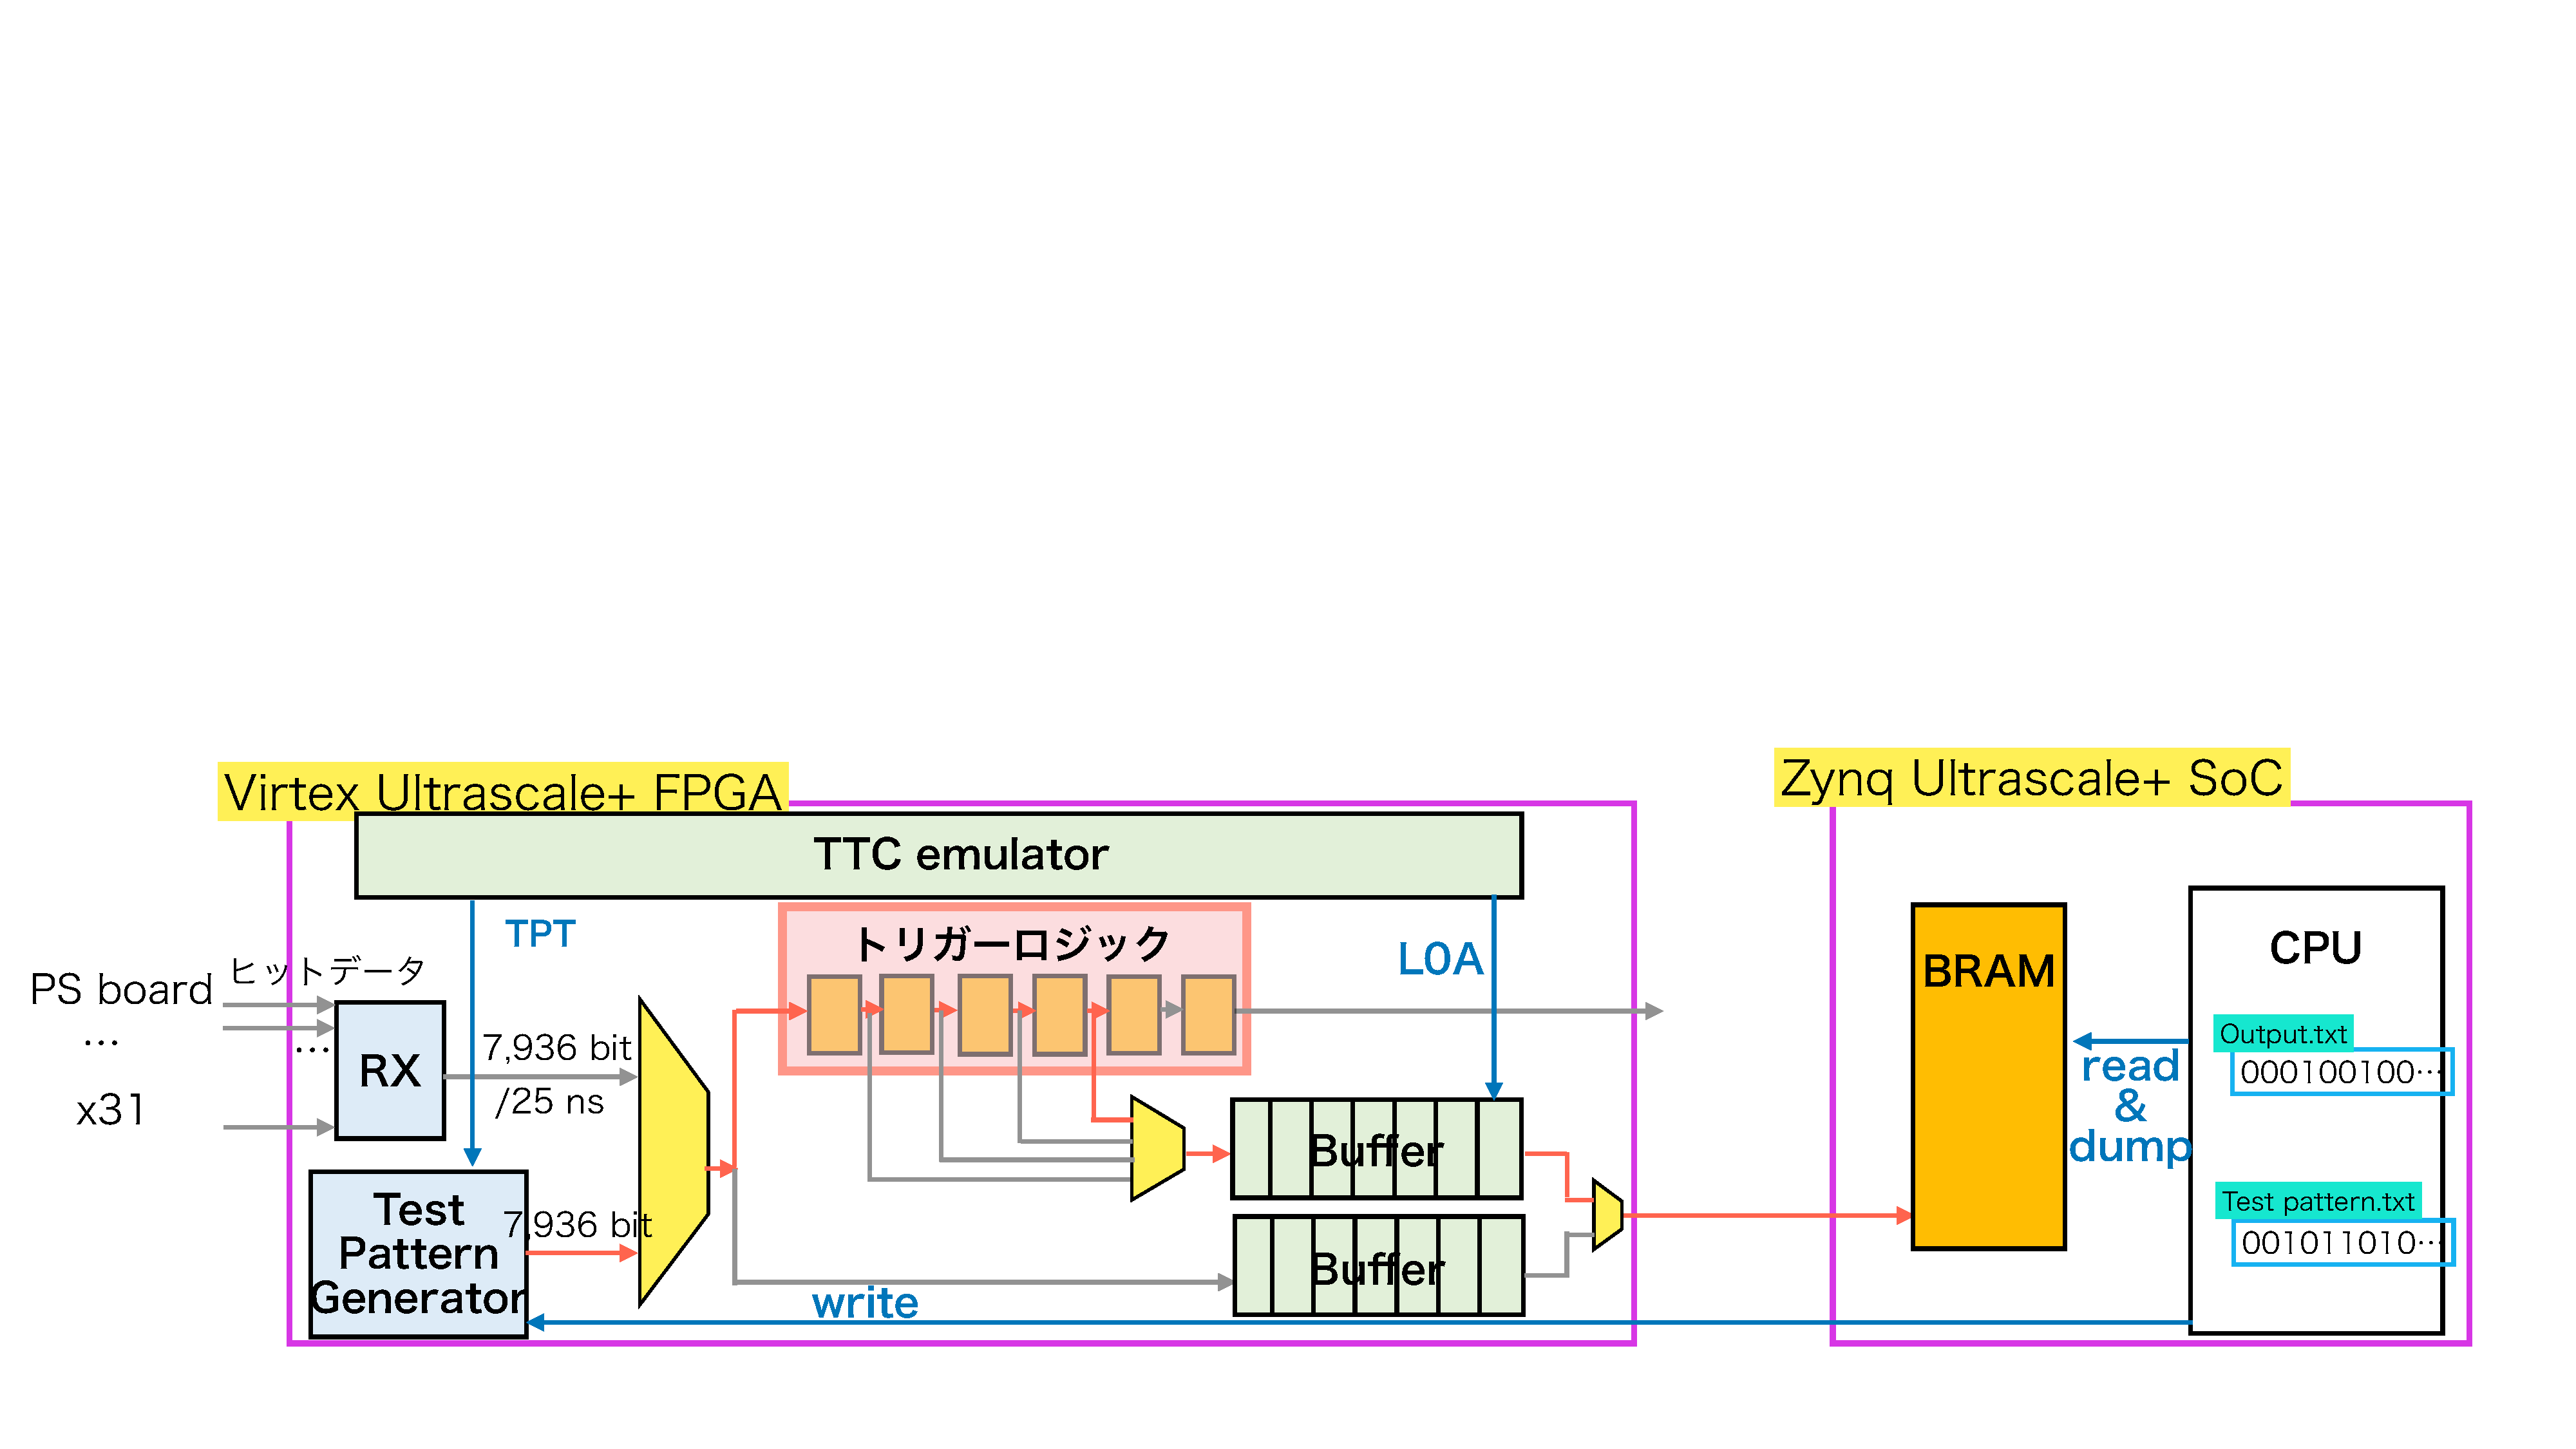
\includegraphics[width=16cm]{fig/Test/TestSystem_overview.pdf}
    \caption[トリガー試験ファームウェアの概要]{トリガー試験ファームウェアの概要。MPSoC上のCPU領域に起動したLinuxを起点に、試験システムのコントロール、データ読み出しを行う。システムはSL上の水晶発振器で生成した40.079 MHzクロックをLHC陽子バンチ交差クロックの代わりに利用する。FELIXから分配されるTPT、L0A、BCRなどのTTC信号はSL内部のTTC emulatorで生成する。トリガー回路へのヒットビットマップの入力はTest Pattern Generatorから行う。トリガー回路の出力は読み出し回路を通じてMPSoC上のBRAMにダンプし、それをLinuxから読み出すことでトリガー演算結果を取得する。}
    \label{TestSystem_Overview}
\end{figure}

トリガー回路へのデータ入力はTest Pattern Generatorが担う。Test Pattern GeneratorはPS boardから受信するヒットビットマップをエミュレートした試験用データ (テストパターン、合計256 bit x 31 PS board = 7936 bit /BC) をBRAMに格納し、TPTごとに1 BC分のデータをトリガー回路に入力する。このように、PS board からの出力自体をエミュレートするシステムにすることで、Channel Mapping からTrack Selectorまでトリガー回路全体を試験することができる。またこの設計により、元のデータセットの種類に関わらず、任意のデータセットをテストパターンとして統一的に扱うことができ、汎用的な利用が可能となっている(テストパターンの作成方法は後述する)。さらに、Test Pattern Generator 内のBRAMはMPSoC上のLinuxから何度でも書き換えることができるため、任意のイベント数で試験を行うことができる。

トリガー回路にはその中間データをプローブするための読み出し回路を実装する。トリガーアルゴリズムの適した箇所で、適した情報を選択的に読み出す機構を実装することにより、トリガー回路内部で行われた処理を系統的に調査することが可能である。中間データは読み出し回路内部で効率的に圧縮され、データ量を削減した上で、高速チップ間通信を利用してMPSoCへ送られる。

\subsection*{Test Pattern Generator}
Test Pattern Generator は幅 128 bit、深さ 64 列 のBRAMにテストパターンを保存し、TTC emulatorからTPTが供給されたタイミングで1BC分のデータをトリガー回路に投入する。1つのBRAMがPS board 1リンク分の信号を保存する。全31 PS board $\times$ 2リンクの信号をエミュレートするため、Test Pattern Generatorには合計62個のBRAMが並列に配置される。

BRAMにはcoe形式のファイルを利用して初期値を設定できるほか、MPSoCから何度でもテストパターンを上書きすることができる。そのため、BRAMの深さに制限されることなく任意のイベント数を用いた試験を行うことができる。以下にそれぞれの昨日の実装について述べる。


\subsection*{トリガー回路中間状態の読み出し回路}
6段階のトリガーモジュールで構成されるトリガー回路には、各モジュールの出力をプローブするための読み出し回路を実装する。トリガー読み出しでは、トリガーモジュール間で渡されるデータの中から、アルゴリズムを調査する上で必要なデータのみを選択的に読み出すことで、効率の良い論理回路の検証ができるようになっている。

例としてWire Strip Coincidenceの出力として読み出すデータを説明する。Wire Strip Coincidenceは8 Unit regionから1 つのミューオン候補を、32 Unit regionから4 つのミューオン候補をそれぞれ出力し、最大180個のミューオン飛跡候補をInner Coincidenceに送る。読み出し回路はこの最大180個のミューオン候補を並列に読み出せるよう設計しており、各領域ごとに表\ref{tab:WS_format}のフォーマットに飛跡情報を成形する。各モジュールの出力のうち、最上位1 bitをvalid信号として定義する。後段のCandidate Selectorはvalid信号が立てられた領域の情報のみを選択的に読み出すため、効率的にデータを削減することができる。

\begin{table}[]
    \centering
    \caption[Wire Strip Coincidenceの読み出しフォーマット]{Wire Strip Coincidenceの読み出しフォーマット。}
    \label{tab:WS_format}
    \begin{tabular}{|c|c|}
    \hline
    \# of bits & Name                                                                                        \\ \hline\hline
    1          & The flag indicates that the region has received at least one wire segment and strip segment \\ \hline
    4          & $p_{\mathrm{T}}$ threshold reconstructed using Coincidence                                  \\ \hline
    3          & Reserved                                                                                    \\ \hline
    7          & $\Delta\theta$ from Wire Segment Reconstruction                                             \\ \hline
    2          & Number of stations with the hits used for wire segment                                      \\ \hline
    4          & $\Delta\phi$ from Strip Segment Reconstruction                                              \\ \hline
    2          & Number of stations with the hits used for strip segment                                     \\ \hline
    1          & Reserved                                                                                    \\ \hline
    \end{tabular}
\end{table}


それぞれのモジュールから読み出すデータの出力ビット幅を表\ref{tab:output_width}に示す。読み出し回路において、数千ビットの信号を一度に処理しようとすると、タイミング制約を満たしてロジックを配置することが難しくなる。そこでbit幅が大きな信号線については、いくつかの並列な処理レーンに分割して読み出しを進める。また、全てのトリガーモジュールの読み出し回路を同時に実装するのはリソースの観点で不可能である。そのため、目的に応じてどのトリガーモジュールの出力を読み出すか選択し、ファームウェアを分けて試験を行う。読み出し回路の概要を図\ref{Readout_Circuite}に示す。以下に各モジュールの役割を説明する。

\begin{table}[]
    \centering
    \caption[各モジュールの出力ビット幅]{各モジュールの出力ビット幅。}
    \label{tab:output_width}    
    \begin{tabular}{|c|c|c|c|}
    \hline
    トリガー回路                                      & SLR & 出力ビット幅 (bits) & レーン数 \\ \hline\hline
    \multirow{3}{*}{Channel Mapping}               & 0   & 2732          & 4    \\ \cline{2-4} 
                                                  & 2   & 2732          & 4    \\ \cline{2-4} 
                                                  & 3   & 1000          & 2    \\ \hline
    \multirow{3}{*}{Wire Station Coincidence}     & 0   & 1768          & 3    \\ \cline{2-4} 
                                                  & 2   & 1768          & 3    \\ \cline{2-4} 
                                                  & 3   & 804           & 3    \\ \hline
    \multirow{3}{*}{Strip Station Coincidence}    & 0   & 1890          & 3    \\ \cline{2-4} 
                                                  & 2   & 1890          & 3    \\ \cline{2-4} 
                                                  & 3   & 378           & 3    \\ \hline
    \multirow{3}{*}{Wire Segment Reconstruction}  & 0   & 3404          & 5    \\ \cline{2-4} 
                                                  & 2   & 3404          & 5    \\ \cline{2-4} 
                                                  & 3   & 1472          & 2    \\ \hline
    \multirow{3}{*}{Strip Segment Reconstruction} & 0   & 360           & 1    \\ \cline{2-4} 
                                                  & 2   & 360           & 1    \\ \cline{2-4} 
                                                  & 3   & 72            & 1    \\ \hline
    \multirow{3}{*}{Wire Strip Coincidence}       & 0   & 1776          & 3    \\ \cline{2-4} 
                                                  & 2   & 1776          & 3    \\ \cline{2-4} 
                                                  & 3   & 768           & 1    \\ \hline
    \end{tabular}
\end{table}

\begin{figure} 
\centering
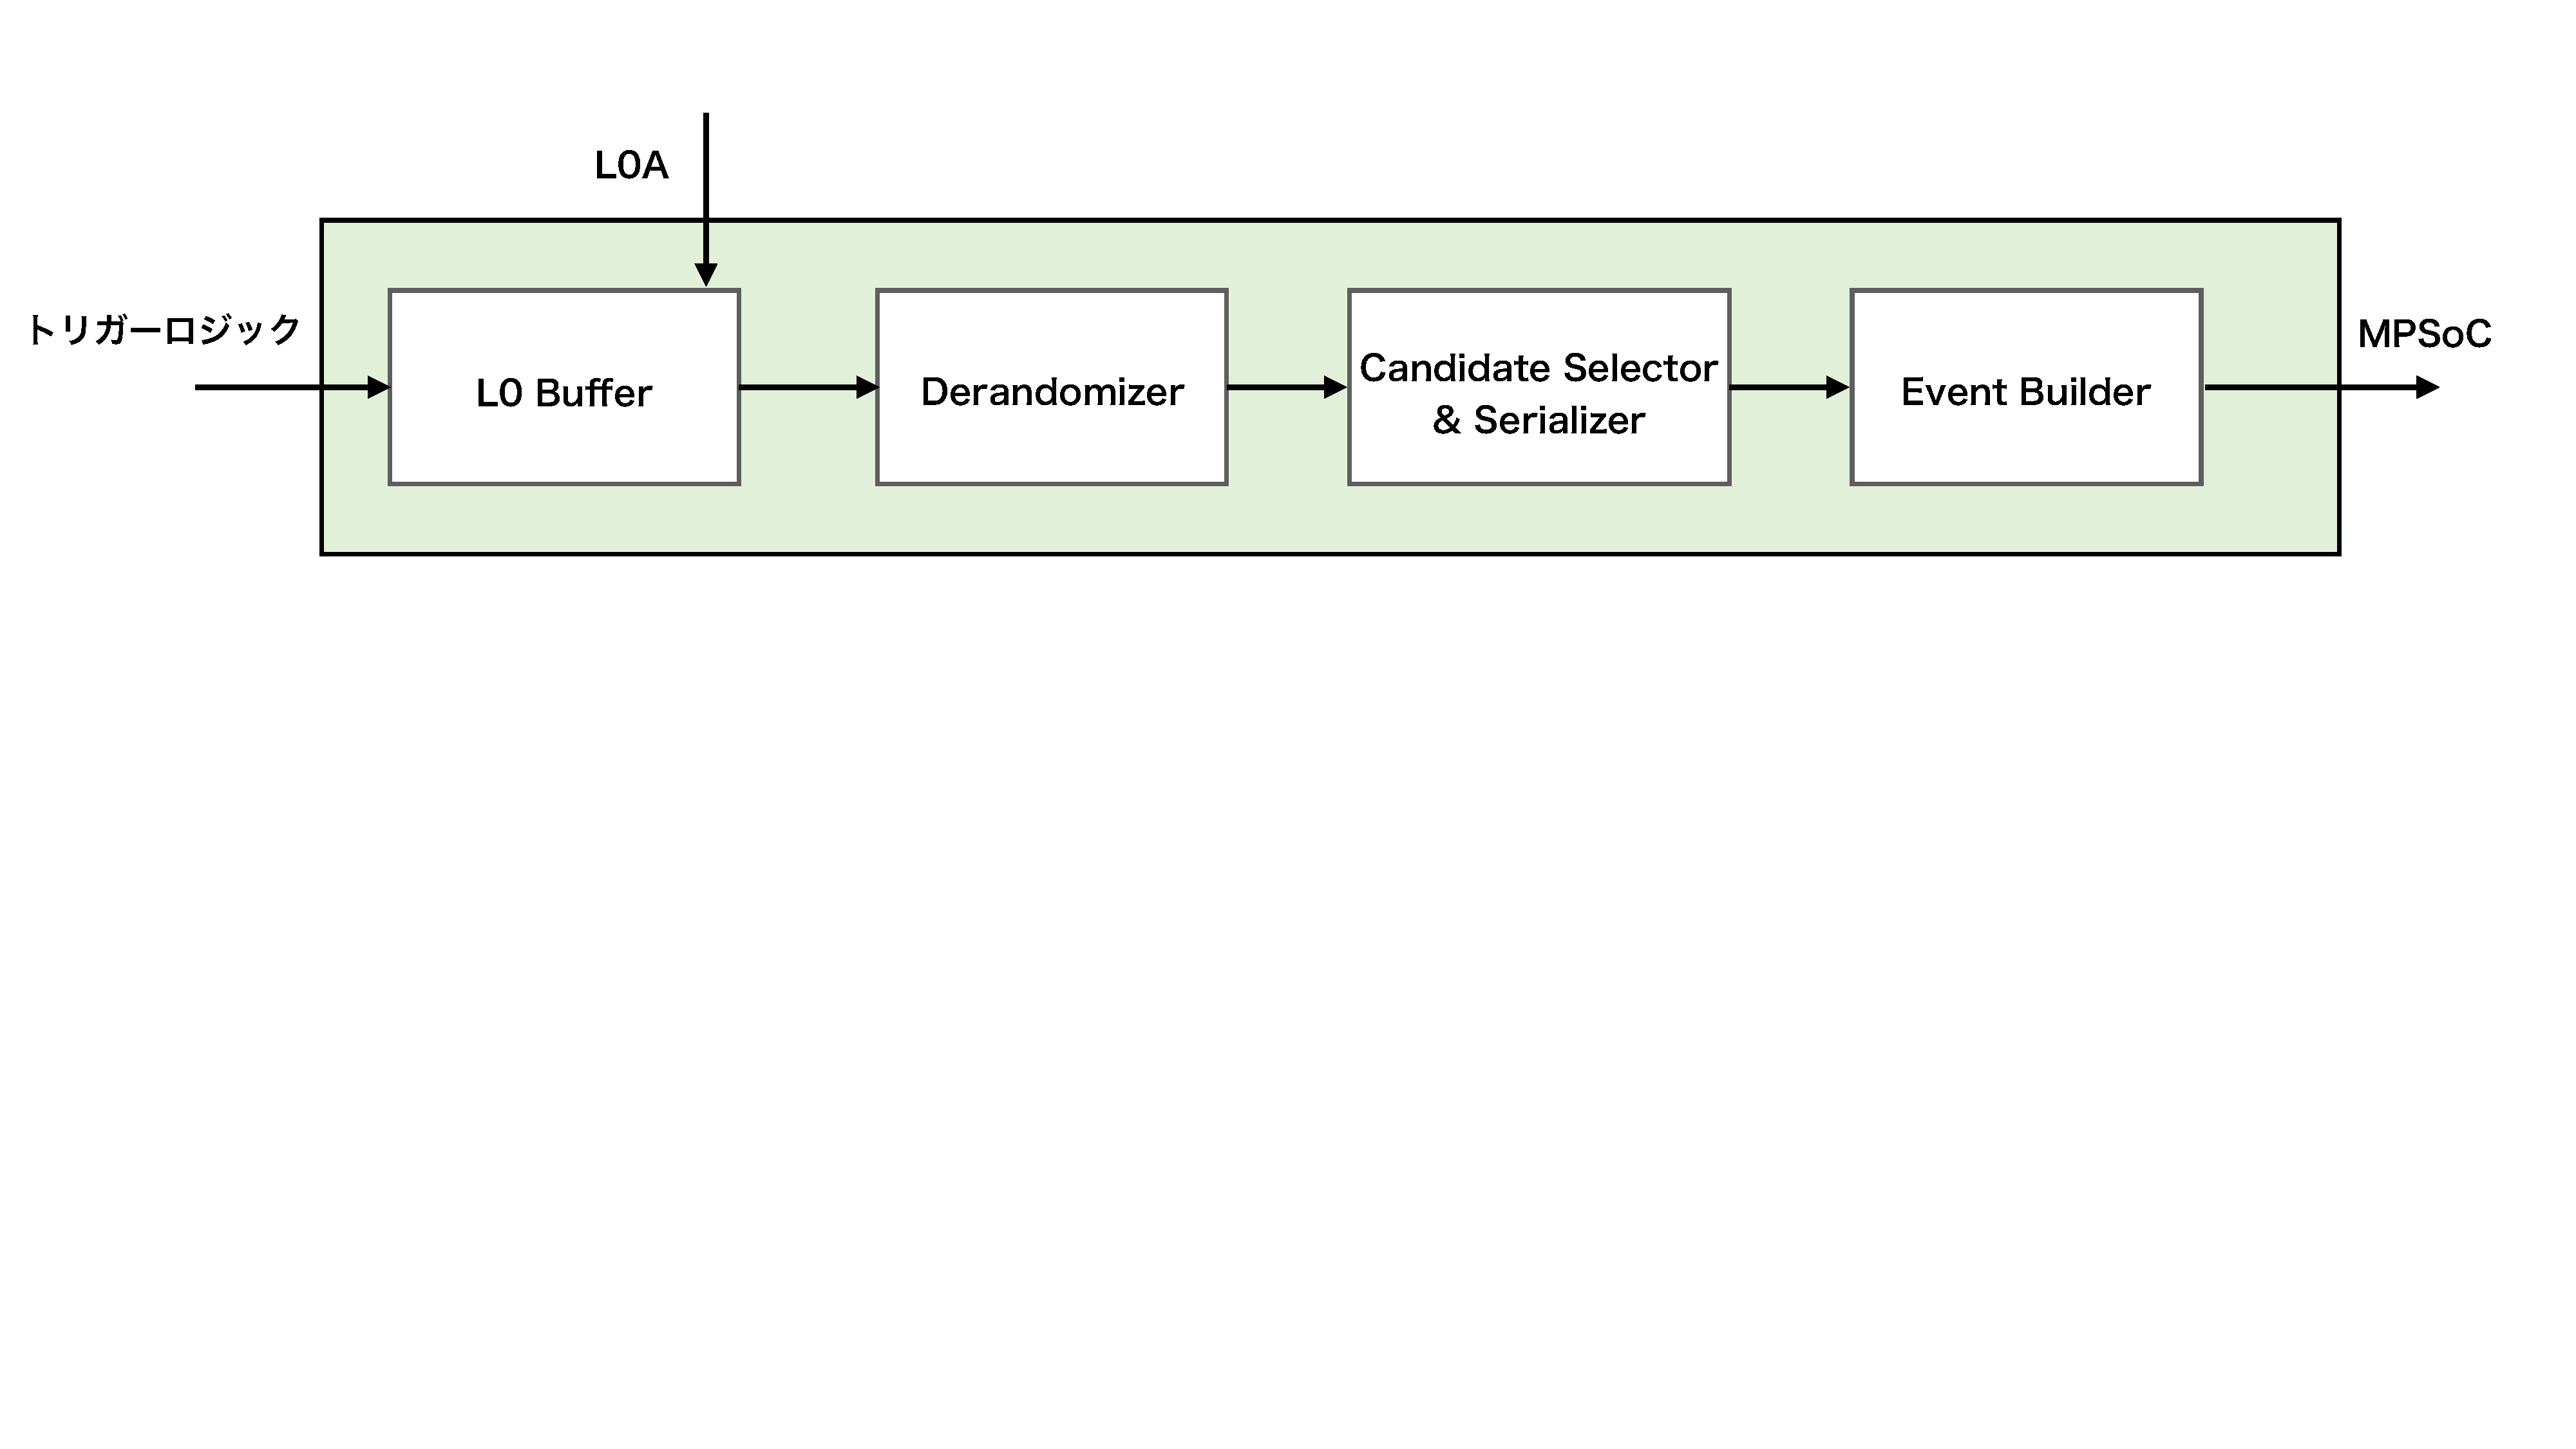
\includegraphics[width=16cm]{fig/Test/Readout_Circuite.pdf}
\caption[トリガー読み出し回路の概要]{トリガー読み出し回路の概要。トリガー回路からの出力はL0 Bufferに格納され、L0Aが出されたイベントのみDerandomizerに送信される。トリガーモジュールからの出力は、すべてのユニットからの出力を並列に並べてあるが、Candidate Selectorはこの中から飛跡を再構成できたユニットからの出力のみを抜き出して、Event Builderに送信する。Event Builderでは複数のモジュールからの出力を1つのパケットにまとめて、MPSoCへと送る。}
\label{Readout_Circuite}
\end{figure}

\subsubsection*{L0 Buffer}
    トリガー読み出しに際してフォーマットされたデータはL0 Bufferにダンプされる。L0 Bufferは入力ビットマップと同じ幅をもつ深さ512 列のBRAMあり、TTC emulatorからL0Aが出されるまでのバッファリングを行う。トリガーモジュールには40 MHz、160 MHz、240 MHzで駆動するものが存在するが、いずれのモジュールでも1つの陽子バンチ交差由来の出力は25 nsごとに横並びに揃えられ、40 MHzのLHC クロックで動作する書き込みポインタに従って、L0 Bufferに格納される。一方、読み出しは240 MHzで行われ、読み出されたデータはDerandomizerに送られる。

\subsubsection*{Derandomizer}    
    Derandomizerは入力ビットマップと同じbit幅をもつ深さ 512 列 のFIFOで、後段で行われる圧縮およびシリアル化の処理待ち用バッファーとして動作する。後段のCandidate Selector から読み出し命令を受け取るたびに、FIFOの先頭のイベントを出力する。

\subsubsection*{Candidate Selector \& Serializer}
    Candidate Selectorは各トリガーモジュールのすべてのユニットから出力される飛跡候補の中から、ミューオン候補を再構成できたユニットの出力のみを選択して後段に送る。これにより大幅なデータ削減が達成される。選択された飛跡情報には、どのサブユニットからの出力かを示す6 bitの識別IDと2bit のbunch tagが付与され、32 bit幅のワードとして後段のSerializerに送信される。
    Serializerは32 bit幅のワードをクロックチックごとに1ワードずつ処理し、あるL0Aに対応する1イベント分のパケットをまとめて、後段のEvent Builderに渡す。図\ref{tab:packet_format}にパケットのフォーマットを示す。パケットにはイベント境界を示すための特別なワード Start of Event (SOE)、End Of Event (EOE) が挿入される。

    \begin{table}
        \centering
        \caption[パケットのフォーマット]{SerializerからEvent Builderに送られるパケットのフォーマット}
        \label{tab:packet_format}
        \footnotesize
        \scalebox{0.7}[0.8]{
        \begin{tabular}{|c|cccccccccccccccccccccccccccccccc|}
        \hline
                & \multicolumn{1}{c|}{31} & \multicolumn{1}{c|}{30} & \multicolumn{1}{c|}{29} & \multicolumn{1}{c|}{28} & \multicolumn{1}{c|}{27} & \multicolumn{1}{c|}{26} & \multicolumn{1}{c|}{25} & \multicolumn{1}{c|}{24} & \multicolumn{1}{c|}{23} & \multicolumn{1}{c|}{22} & \multicolumn{1}{c|}{21} & \multicolumn{1}{c|}{20} & \multicolumn{1}{c|}{19} & \multicolumn{1}{c|}{18} & \multicolumn{1}{c|}{17} & \multicolumn{1}{c|}{16} & \multicolumn{1}{c|}{15} & \multicolumn{1}{c|}{14} & \multicolumn{1}{c|}{13} & \multicolumn{1}{c|}{12} & \multicolumn{1}{c|}{11} & \multicolumn{1}{c|}{10} & \multicolumn{1}{c|}{9} & \multicolumn{1}{c|}{8} & \multicolumn{1}{c|}{7} & \multicolumn{1}{c|}{6} & \multicolumn{1}{c|}{5} & \multicolumn{1}{c|}{4} & \multicolumn{1}{c|}{3} & \multicolumn{1}{c|}{2} & \multicolumn{1}{c|}{1} & 0 \\ \hline
        SOE       & \multicolumn{5}{c|}{rsvd}                                                                                                       & \multicolumn{4}{c|}{data loss flag}                                                                   & \multicolumn{12}{c|}{0xB0E}                                                                                                                                                                                                                                                                                           & \multicolumn{11}{c|}{L0ID}                                                                                                                                                                                                                                   \\ \hline
        EOE       & \multicolumn{5}{c|}{rsvd}                                                                                                       & \multicolumn{4}{c|}{data loss flag}                                                                   & \multicolumn{12}{c|}{0xB0E}                                                                                                                                                                                                                                                                                           & \multicolumn{11}{c|}{L0ID}                                                                                                                                                                                                                                   \\ \hline
        data word & \multicolumn{6}{c|}{Unit address}                                                                                                                         & \multicolumn{2}{c|}{BC tag}                       & \multicolumn{24}{c|}{bitmap}                                                                                                                                                                                                                                                                                                                                                                                                                                                                                                                                                                                   \\ \hline
        buffer    & \multicolumn{12}{c|}{0xBFF}                                                                                                                                                                                                                                                                                           & \multicolumn{9}{c|}{rsvd}                                                                                                                                                                                                               & \multicolumn{11}{c|}{L0ID}                                                                                                                                                                                                                                   \\ \hline
        \end{tabular}
        }
    \end{table}

    \subsubsection*{Event Builder}
    上述のCandidate Selectorまでは読み出しレーンごとに処理が行われる。Event Builderはこれらの並列なレーンの出力を直列化し、MPSoCに送信するためのフォーマットに成形する。Serializerから受信する32 bitのワードはEvent Builder内の処理待ちバッファーに格納される。Event Builderは処理待ちバッファーのデータを240 MHzのクロックチックごとに1ワードずつ図\ref{TriggerReadout_format}のフォーマットに成形する。meta switchは読み出しを行うトリガーモジュールの選択状態を表す。meta dataは各トリガーモジュールごとに送られ、そのトリガーモジュールのラベル(data flavor)、読み出しを行うbunch tag (previous, current, next, next to next)の選択状態を表す。
    実機試験ではこのようにFPGA内でエンコードされたデータを、ソフトウェア上で逐次的にデコードすることで、トリガー回路からの出力を一意に再構成して、テキストファイルにダンプする。

    \begin{figure} 
    \centering
    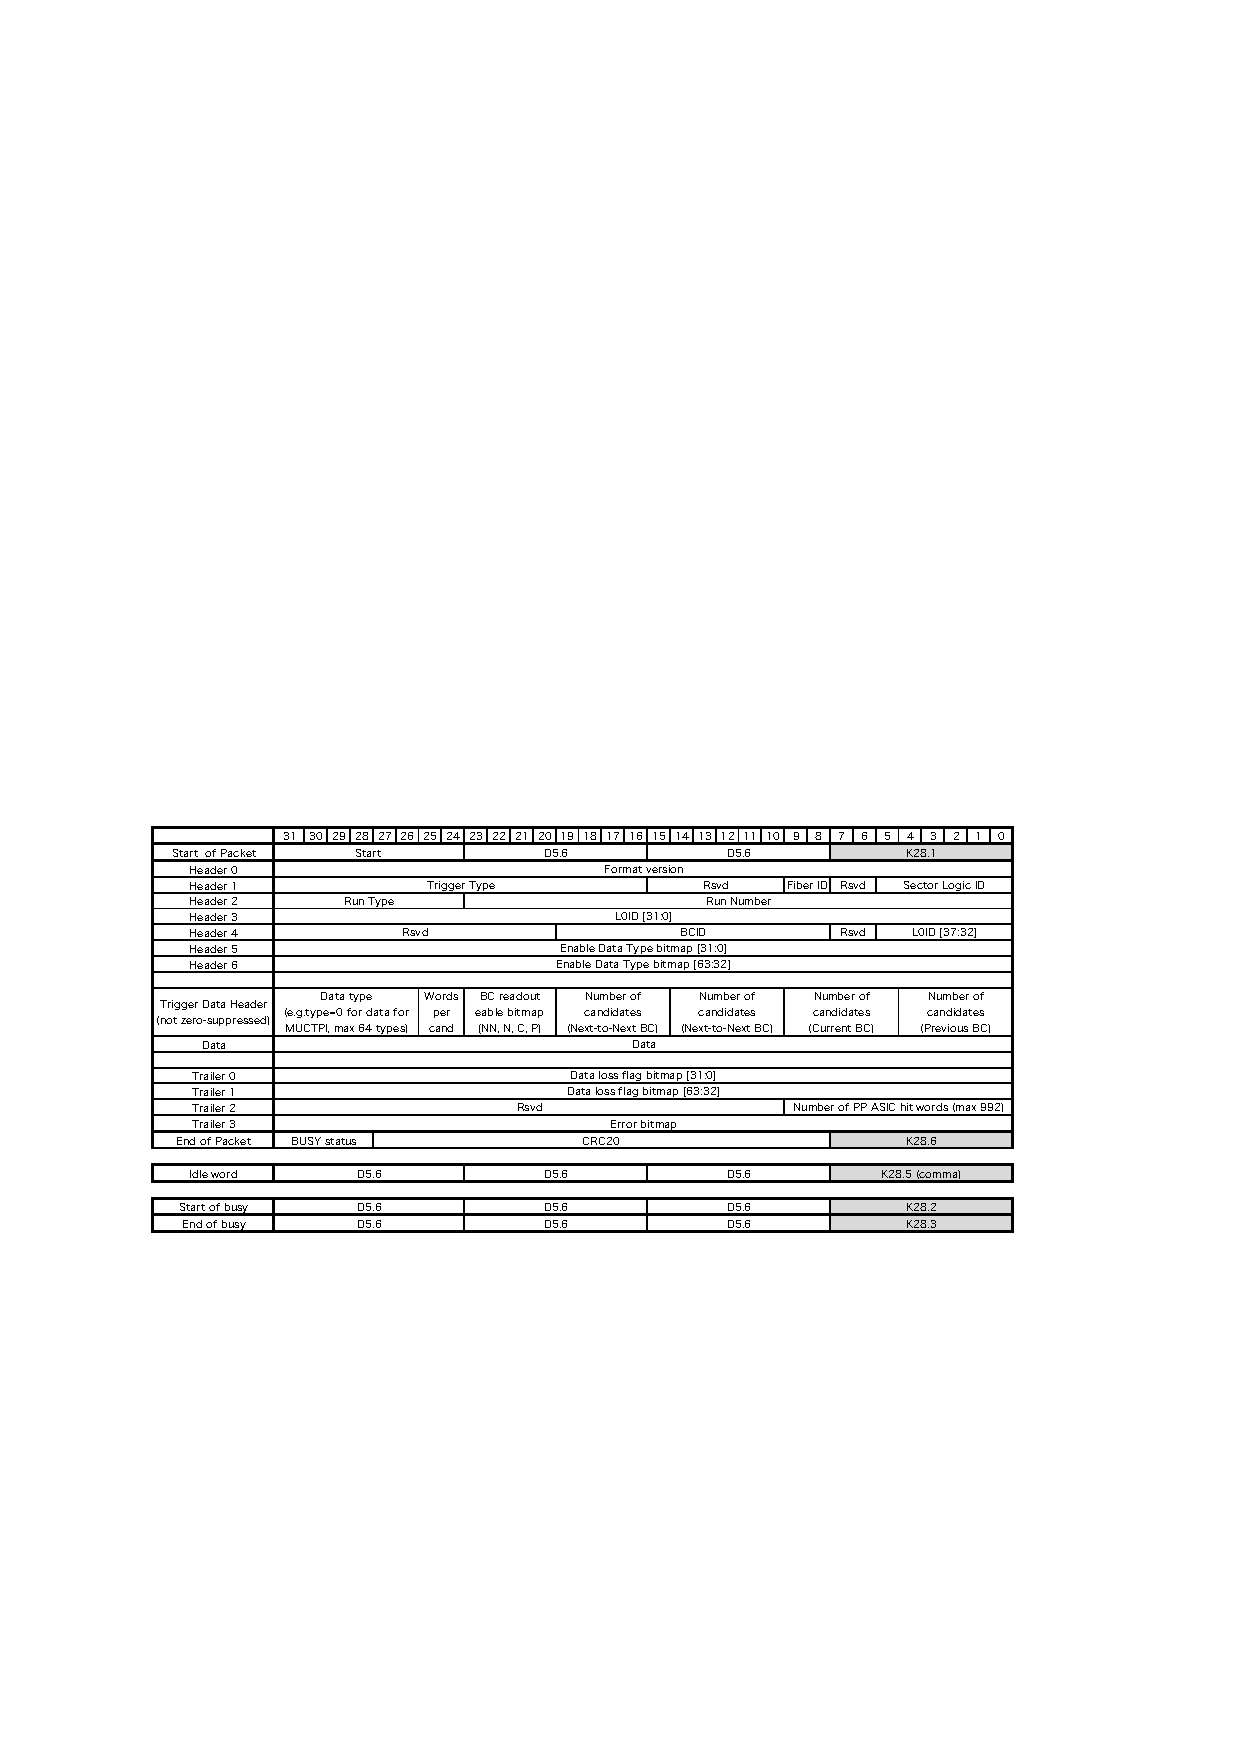
\includegraphics[width=16cm]{fig/Test/TriggerReadout_format.pdf}
    \caption[Event Builderで成形されるトリガー出力のフォーマット]{Event Builderで成形されるトリガー出力のフォーマット\cite{SLPDR}}
    \label{TriggerReadout_format}
    \end{figure}

\subsection*{SL FPGAからMPSoCへのデータ転送}
SL FPGAで成形されたデータはMPSoC PL領域内のBRAMに格納されたのち、PSから読み出される。SL FPGAからMPSoCへのデータ転送は、高速シリアル通信を利用する。図\ref{C2C}にチップ間通信の概要を示す。
\begin{figure} 
\centering
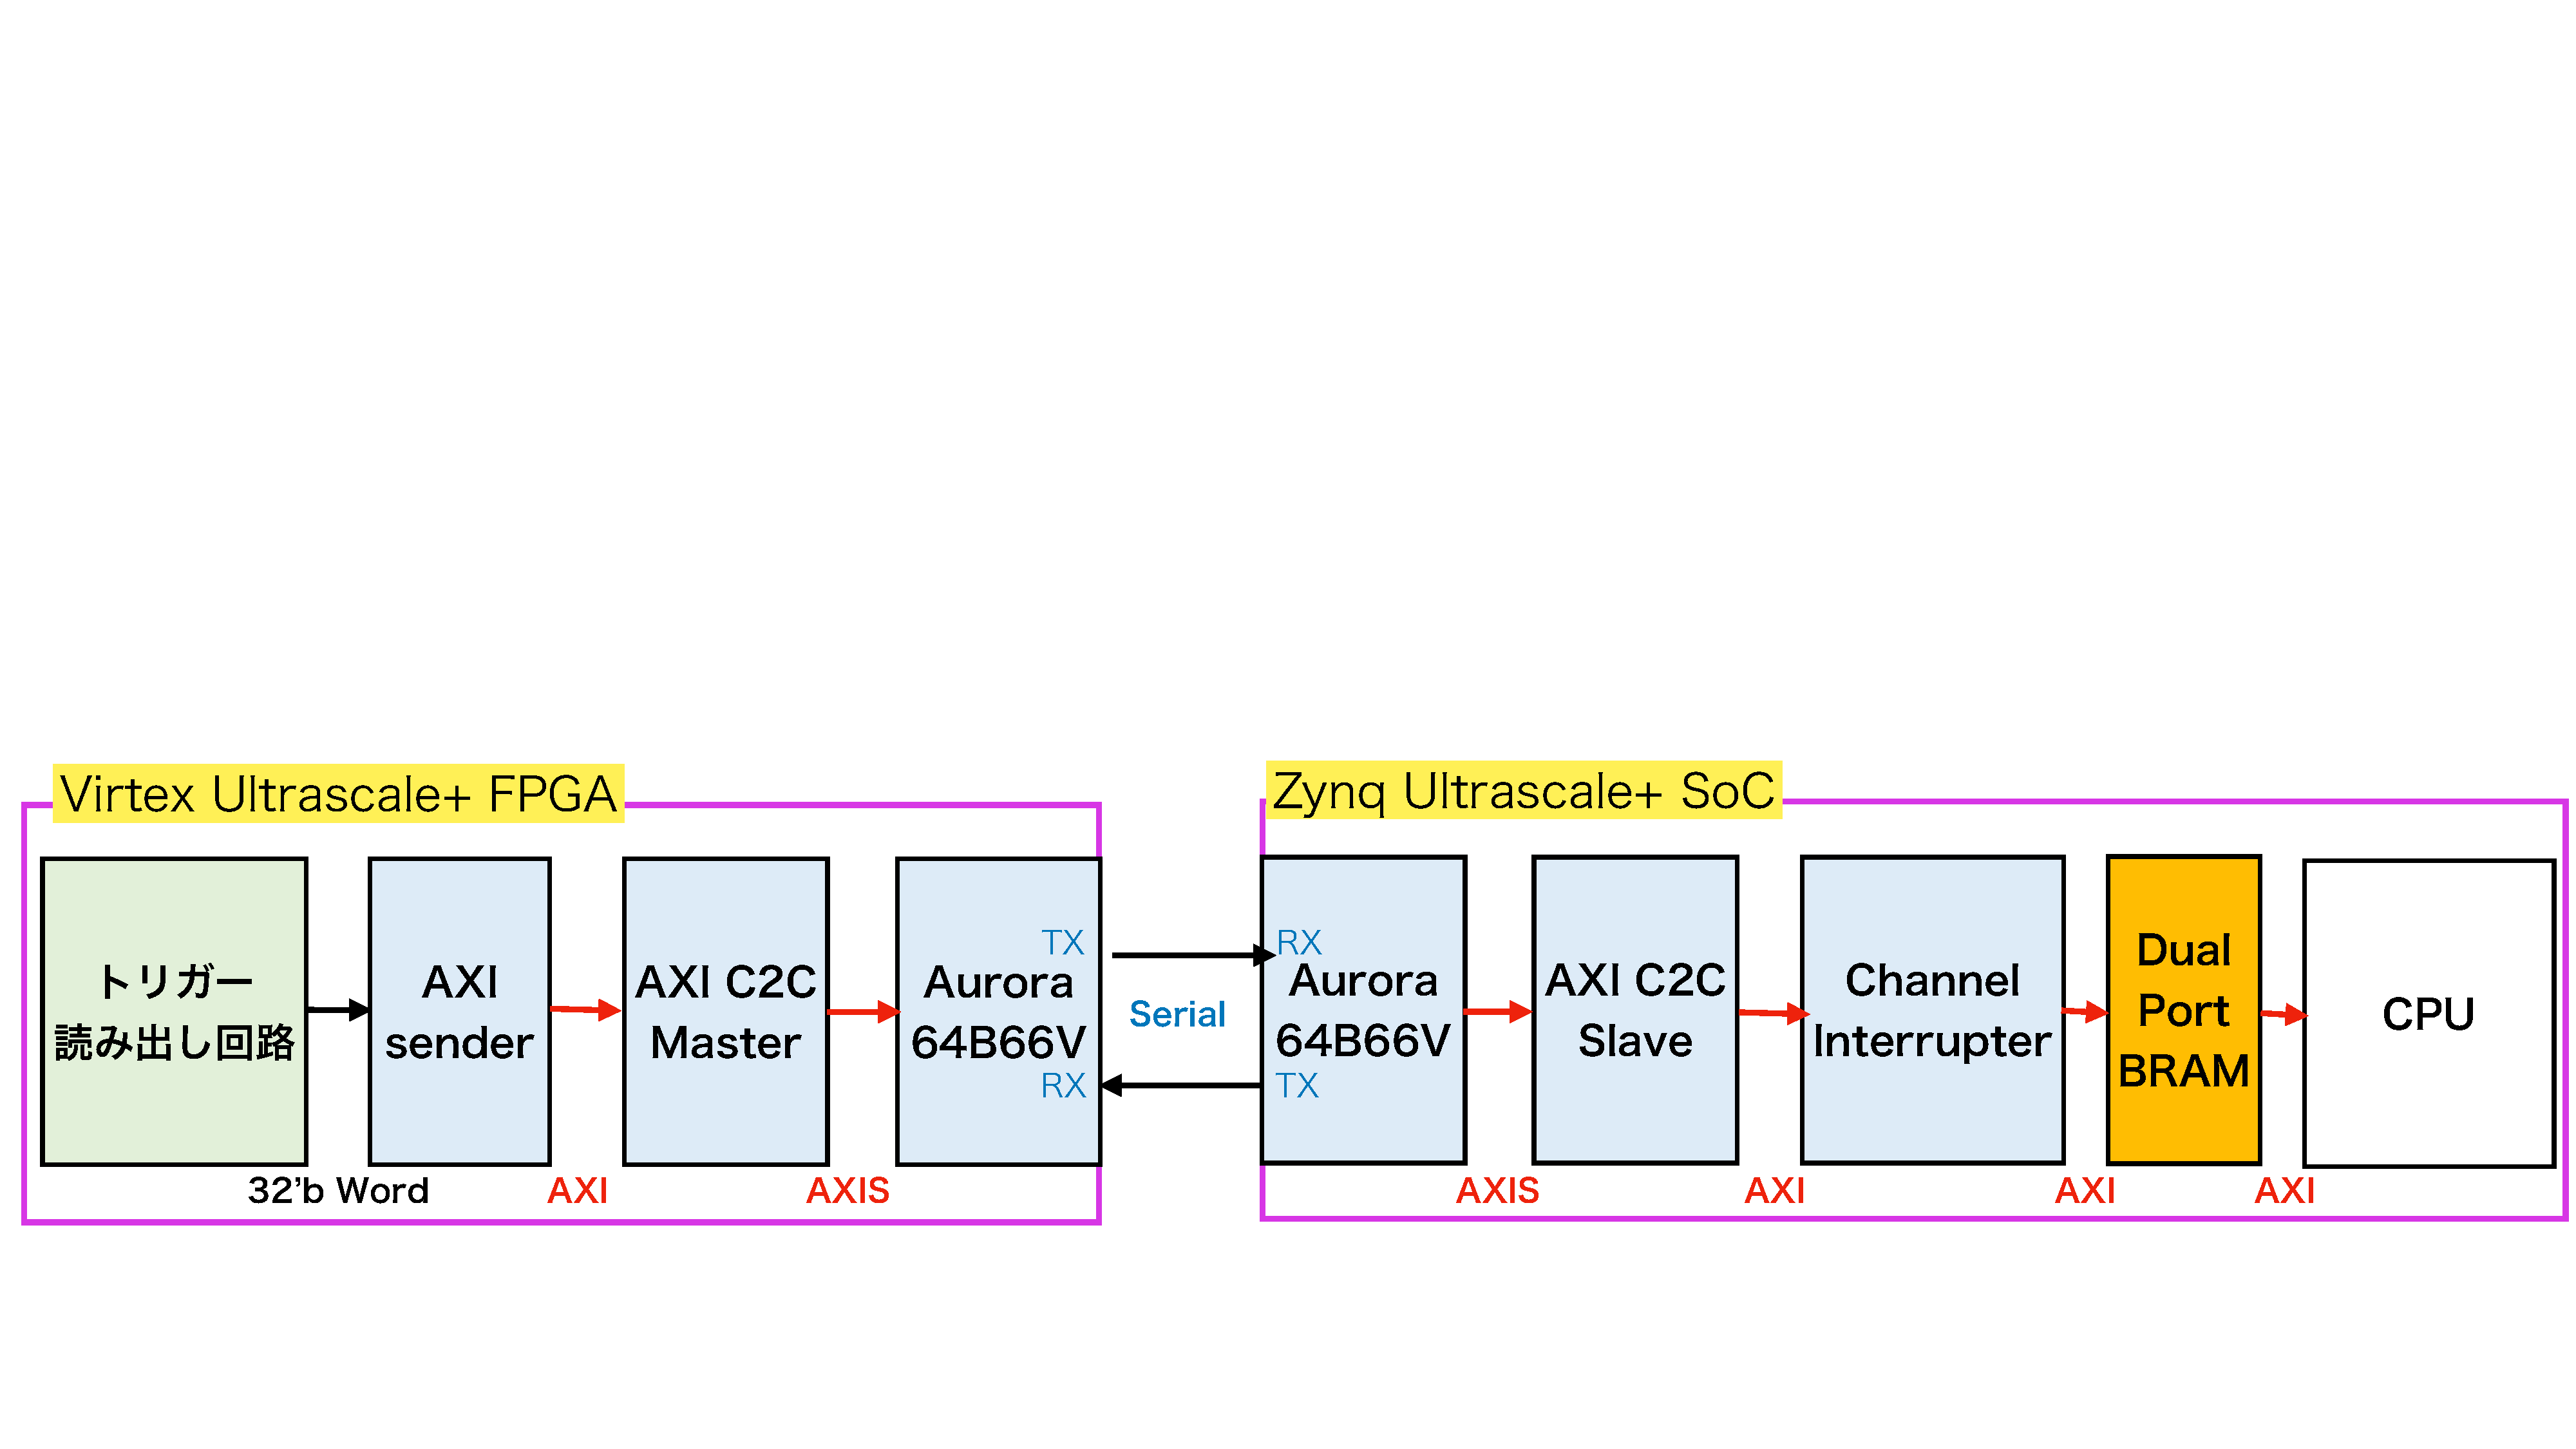
\includegraphics[width=16cm]{fig/Test/C2C.pdf}
\caption[SL FPGAからMPSoCへのチップ間通信]{SL FPGAからMPSoCへのチップ間通信。トリガー回路からの出力はAXI sender からAXI プロトコルに乗せられ、Aurora64B66Vでシリアル通信のデータにエンコードされ、MPSoCへ送られる。そのデータはMPSoCで再びAXIに載せ替えられ、BRAMにダンプされる。}
\label{C2C}
\end{figure}

Event Builderから出力される32 bit幅のワードはAXI senderに送られる。AXI senderは受信したデータをデータ幅32 bit、アドレス幅 32 bitのバス通信であるAXIプロトコルで、AXI chip2chipへ送る。AXI chip2chipはAXI形式のデータをAXI Stream 形式に変換し、Aurora 64B/66B Masterと通信する。AXI chip2chip以降のデータ転送ではAXIバーストと呼ばれる、連続したデータブロックを高速転送するための手法が採られている。AXIバーストはMasterからSlaveに送信するワード数を事前に定義 (本システムでは256ワード) することで、通常のハンドシェイキングで生じるバスのアイドルタイムを最小限にする。
Aurora 64B/66B MasterはAXI Stream形式のデータをシリアル通信のデータにエンコードし、ギガビットトランシーバーを用いてチップ間通信を行う。

シリアルデータは、MPSoCのPLに実装されたAurora 64B/66B Slaveで受信され、再びAXI Stream形式にデコードされた後、AXI chip2chip でAXI 形式へと変換される。MPSoCでAXI形式に戻されたデータはChannel Interrupterを中継して、幅32bit、深さ8192 列 のDual port BRAMにダンプされる。BRAMのもう片方のポートはMPSoCのPSにAXI形式で接続されており、BRAMを介してPLからPSへのデータ送信が可能になっている。AXIバーストを利用していることで1イベント当たりのワード数は256に固定されている。そのため、BRAMに格納できるイベント数も固定であり、最大$ \,8192 / 256 = 32\,$ イベントである。一度BRAMがfullになった場合でも、MPSoCからマニュアルでリセットをかけることで、データ取得を再開できる。

\subsection*{アプリケーションの概要}
シングルボードのトリガー試験を行うために開発した、MPSoC上で走るアプリケーションの概要を説明する。このアプリケーションはSLのSDカード上にテキストファイルとして保存されたLUTやテストパターンをハードウェアに書き込み、トリガー演算の結果をSDカード上のテキストファイルにダンプする。
図\ref{Flowchart}にアプリケーションのフローチャートを示す。

\begin{figure} 
\centering
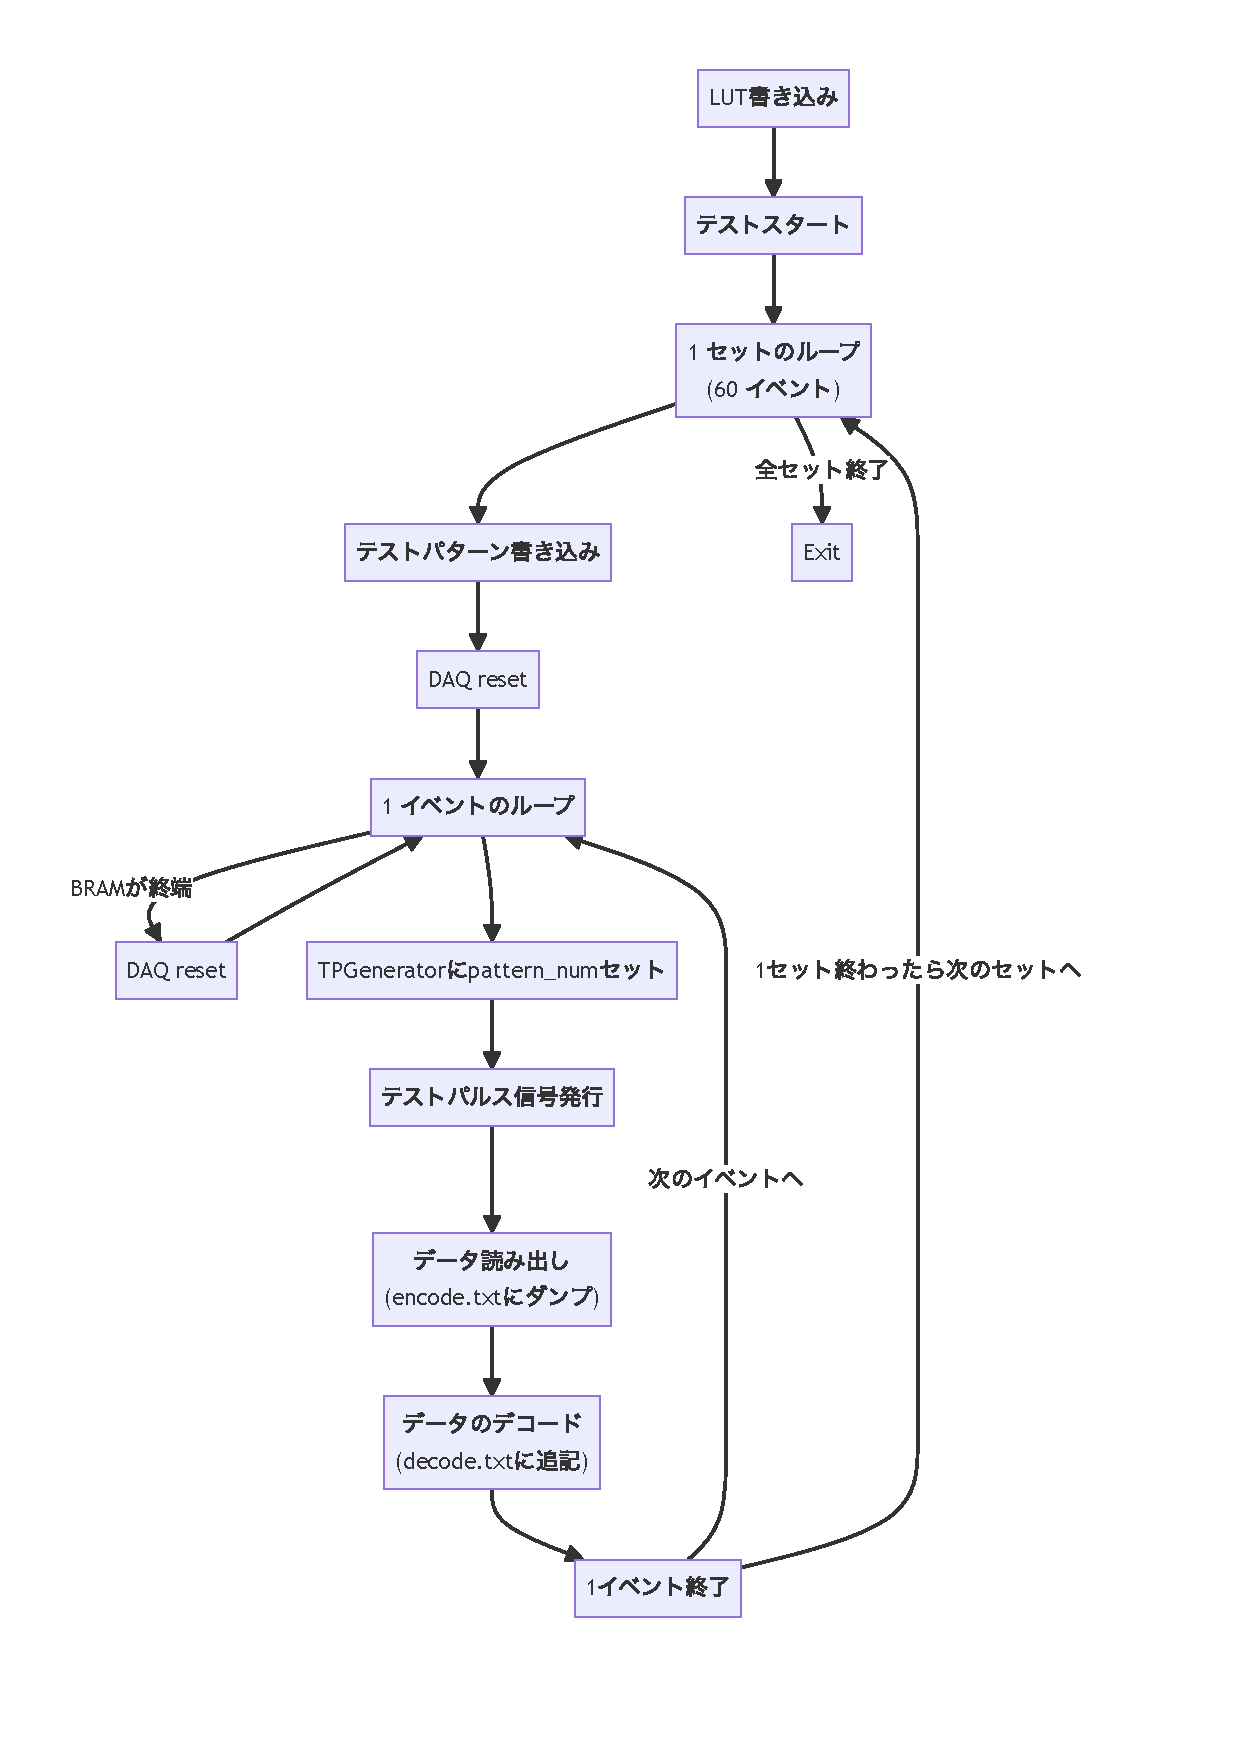
\includegraphics[width=10cm]{fig/Test/Flowchart.pdf}
\caption[アプケーションのフローチャート]{アプリケーションのフローチャート。Test Pattern GeneratorのBRAMの容量に合わせて、60イベントを1セットに試験を行う。1イベントのループでは、テストパルス信号の発行、データ読み出し、データのデコード、テキストファイルへのダンプを行う。}
\label{Flowchart}
\end{figure}

試験の最初にはLUTの書き込みを行う。LUTに利用されているURAMはファームウェア上で初期値を設定することができないため、ファームウェアのリセットのたびに書き込みを行う必要がある。Wire Strip CoincidenceまでのすべてのLUTを書き込むのに、概ね20分程度要する。

試験はTest Pattern Generatorに一度に書き込めるイベント数である60イベントを1セットとして、テストパターンの書き込みと60イベント分のテストを繰り返す。1イベントのループでは、最初にTest Pulse Generatorのパターンナンバーを指定し、60イベントの中からトリガー回路に投入するイベント番号を指定する。次にマニュアルでテストパルス信号を駆動し、トリガー回路にデータを入力する。トリガー回路の出力は読み出し回路を経てエンコードされたのち、MPSoC上のBRAMに格納される。格納されたデータをMPSoCのPSから取り出し、アプリケーション上でデコードする。得られたビット配列は、最終出力としてSDカード上のテキストファイルにダンプされる。イベントのループを回している過程で、MPSoCのBRAMがfullになった場合はその都度リセットをかける。

試験に要する時間は、LinuxからMPSoC上のFPGAにアクセスするのにかかる時間が律速しており、10,000 イベントの試験におよそ1分程度かかる。

\subsection{トリガー論理回路検証システムの全体像}
\label{subsec_TestSystemOverview}
本研究で開発したシングルボード試験システムに加え、共同研究\cite{mt_yamashita}で開発が進められたテストパターン生成機構、Bitwiseシミュレーターを組み合わせることで、トリガー論理回路を系統的に調査していくための検証システムを構築した。
図\ref{Test_system}に検証システムの全体像を示す。

\begin{figure} 
\centering
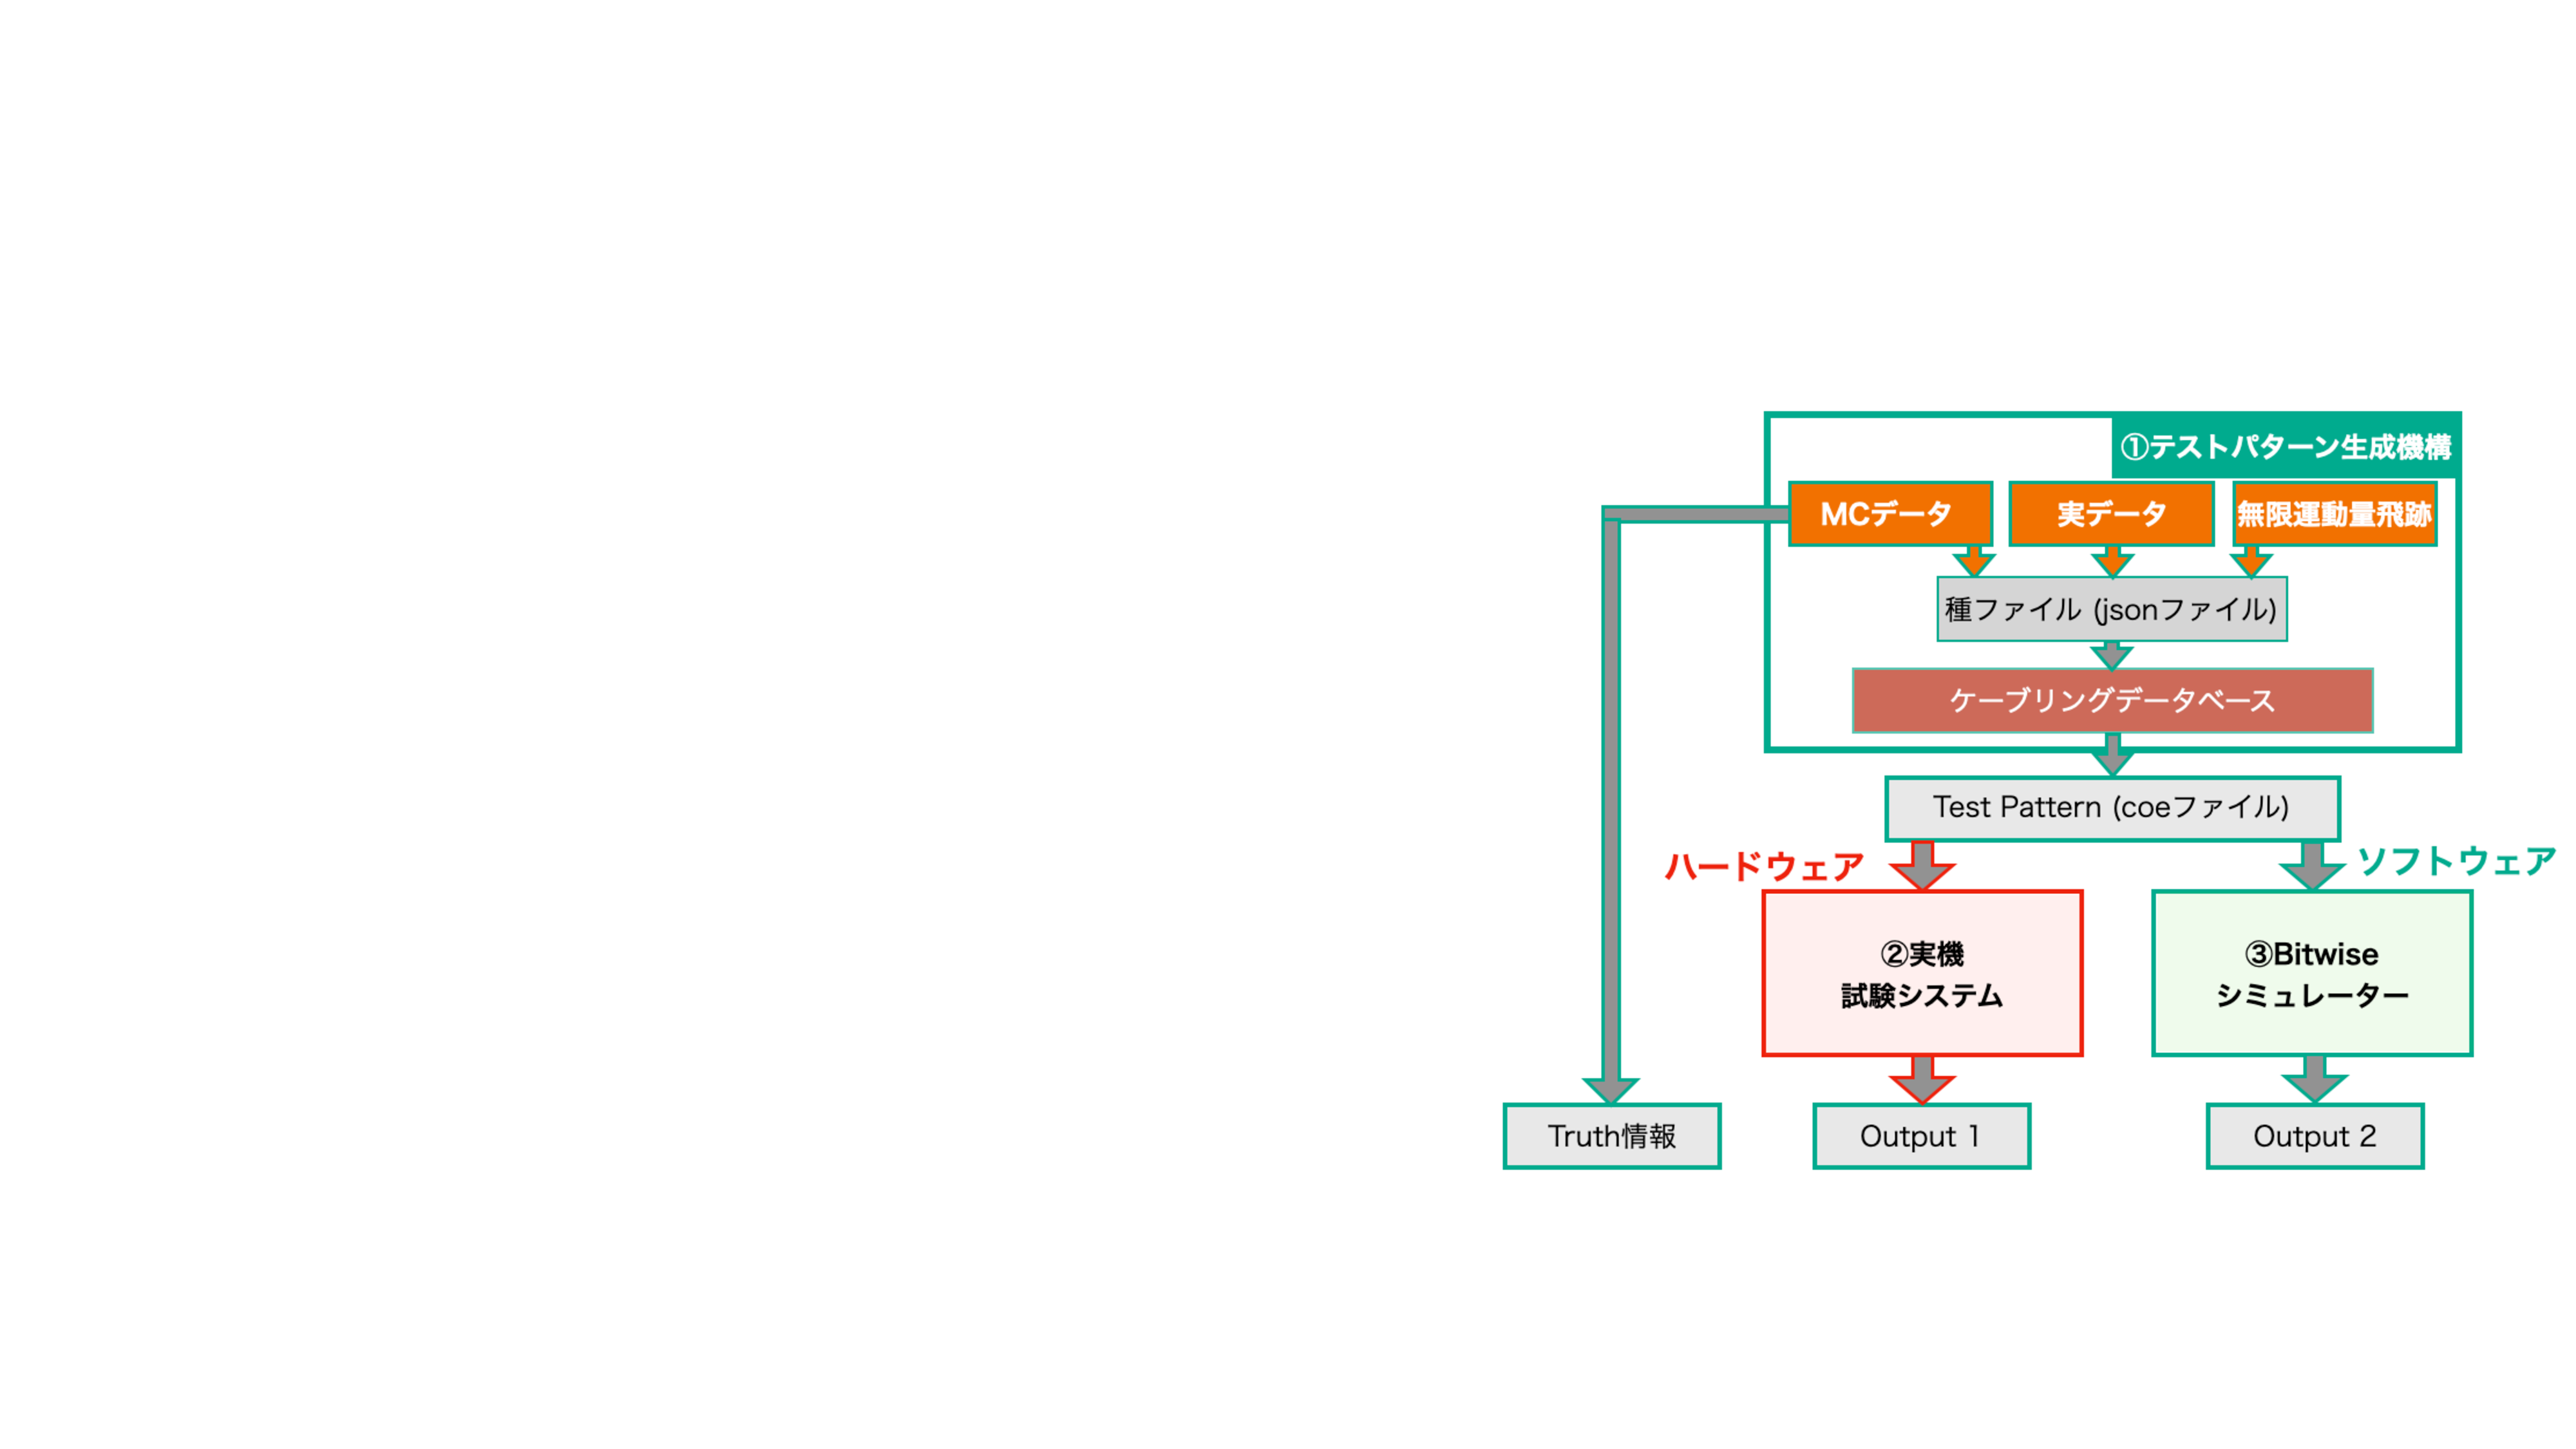
\includegraphics[width=16cm]{fig/Test/Test_system.pdf}
\caption[トリガー論理回路検証機構]{トリガー論理回路検証機構。テストパターン生成機構、SLシングルボード試験システム、Bitwiseシミュレーターで構成される。テストパターン生成機構はMCデータ、実データ、無限運動量飛跡などをもとに、シングルボード試験システムとBitwiseシミュレーターに共通するテストパターンを生成する。シングルボード試験システムはこれを入力として、実機上で動作するトリガー回路の演算結果を出力する。Bitwiseシミュレーターもこれを入力として、トリガー演算をBitレベルで再現したソフトウェアエミュレーターの演算結果を出力とする。この2つの出力を相互に比較・検証することで、トリガー論理回路を系統的に調査する。}
\label{Test_system}
\end{figure}

テストパターン生成機構はシミュレーションデータや実データから、SLが受信するヒットビットマップを再現したテストパターンを作成するツールである。ここではまず、元のデータセットから、TGC検出器のヒットチャンネル情報を抽出し、種ファイルとしてJSONファイルを作成する。次に、種ファイルのデータをTGC検出器からSLまでの複雑な配線情報 (ASD、PS board、SLと続く物理的なケーブルの配線に加え、各デジタル回路内の信号の並び替え情報等も含む) を一元的に管理するケーブリングデータベースと組み合わせ、SLのインプットを再現したテストパターンを生成する。テストパターンはSL実機、Vivado シミュレーション\footnote{実装した論理回路の信号遷移を逐次的にエミュレートするソフトウェア。Vivadoの標準的な機能として実装されている。}、Bitwiseシミュレーターに共通で用いることができるようcoeファイル形式で出力される\footnote{テストパターンを格納するBRAMは、coeファイルによって初期値を設定することができる。そのためVivadoシミュレーションではテストパターンはcoeファイルに格納されているkとが好ましい。これに合わせるように、シングルボード試験システム、Bitwiseシミュレーターもcoeファイルを入力の形式とするよう設計している。}

BitwiseシミュレーターはSLトリガー論理回路をビットレベルで再現したC++ベースのシミュレーターである。このシミュレーターはテストパターンを入力とし、LUTも実機と同じものを使用する。さらに、各トリガーモジュールの出力フォーマットも実機とシミュレーションで統一的に定義しているため、完全に同一のコンフィギュレーションでトリガー演算を行い、その出力をビット単位で比較することができる。Bitwiseシミュレーターはソフトウェアで実装してあるため、実機では出力していないモジュール内部の信号線の情報も簡単に出力することができ、トリガー論理回路のより詳細なデバッグに有用である。

これらの検証システムにより、シミュレーションデータに対するトリガー応答をハードウェアとソフトウェアで計算し、その出力をモジュールごとに系統的に比較・検証する盤石な開発基盤を構築した。以下では、この検証システムを用いて行った、トリガー論理回路の動作検証および性能評価について議論する。




\section{無限運動量飛跡を用いたトリガー回路の動作検証}
\label{sec_IMT}

本章では前節で述べたトリガー回路検証システムと無限運動量飛跡と呼ばれるトイデータセットを用いて行った、トリガー回路の初頭的な動作検証試験について述べる。無限運動量飛跡とは、衝突点から直線的にTGC検出器に入射するミューオンをエミュレートした試験用のイベントであり、トリガーロジックとしては100 \%再構成されることが期待されるイベントセットである。このイベントセットに対するTGC BW コインシデンス(Channel MappingからWire Strip Coincidenceまで)の応答を調べることで、実装したトリガー回路が期待通り動作していることを確かめる。

以下ではまず、テストパターン生成機構に含まれる無限運動量飛跡生成機構について述べた後、試験結果およびその考察について述べる。

\subsection*{無限運動量飛跡生成機構}
\label{subsec_IMT_generation}


前章で述べたようにTGC検出器は位置分解能向上およびデータ量の削減を実現するため、スタッガリング構造を取っている。ステーション内の2層または3層のガスチェンバーは、各チャンネルのカバーする$\eta$領域がずれるよう設置されており、ステーション内コインシデンスにより、位置分解能を2、3倍に高めた代表点を算出する。ここで、M3の各代表点と同じ$\eta$に位置するM1、M2代表点に同じ番号が割り振られるよう定義したものを$\eta$ IDと呼ぶ。$\eta$ IDは各ステーション内の代表点に通し番号的に振られている訳ではなく、M3の代表点を起点に、その$\eta$に一番近い代表点を選ぶようにして値を割り振っている。\footnote{TGC検出器が設計された当初は、各ステーションで$\eta$の位置分解能が均一になるようにワイヤーがバンドルされていたため、ステーション内で通し番号的に$\eta$ IDを割り振ることができるはずだった。しかし、設置の段階でTGC検出器の設置位置が$z$方向にずれたため、これはできなくなった。}

% \begin{figure} 
% \centering
% 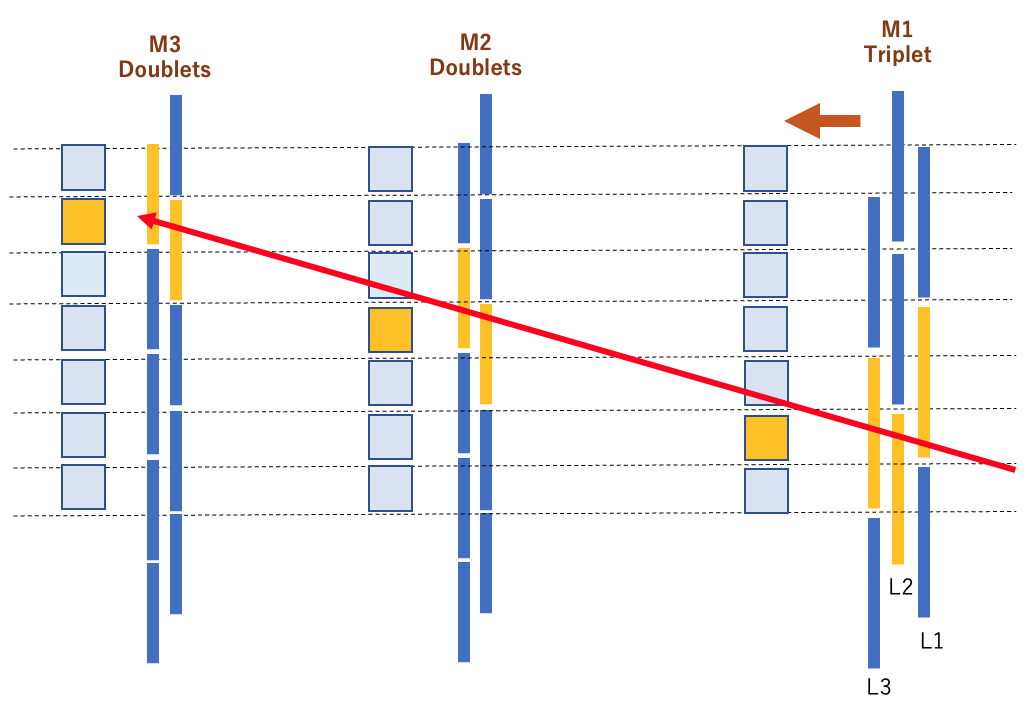
\includegraphics[width=16cm]{fig/Test/StaggerdID.png}
% \caption[$\eta$ IDの概念図]{$\eta$ IDの概念図}
% \label{StaggerdID}
% \end{figure}

$\eta$ IDはケーブリングデータベースにより、各検出器のチャンネル番号と紐づけられている。テストパターン生成機構にはそれらを活用して、任意の2次元座標点に入射する無限運動量飛跡を作成する機構が備わっている。とある($\eta$ , $\phi$)位置に入射するミューオンをエミュレートしたテストパターンが作りたい場合、該当する$\eta$ IDと$\phi$方向の代表点番号 (スタッガードID)を指定するだけで、それに対応する7層分のヒット情報が含まれた、テストパターンが生成される。


\subsection*{無限運動量飛跡試験の概要}
トリガー論理回路および作成されたLUTに対する最初の試験として、無限運動量飛跡に対するトリガー応答を調査した。ここでは論理回路実装やLUT作成の際に生じた不具合を網羅的に洗い出すため、M3のWire、Stripで張られる全ての2次元格子点に対して無限運動量飛跡を用意した。図\ref{InfMomentum}にイベントセットの概念図を示す。1つのSLが担当するTGC 1/24セクターでは、フォワード領域にはM3のWire代表点が243 個、Strip代表点が63 個存在し、合計15,309の2次元格子点が存在する。エンドキャップ領域には$\phi\,$0、$\phi\,$1 それぞれでM3のWire代表点が 579 個、Strip代表点が 63 個存在し、合計36,477の格子点が存在する。このイベントセットに対する、Wire Segment Reconstruction、Strip Segment Reconstruction、Wire Strip Coincidenceの応答を調べることで、トリガー回路の動作を調査した。



\begin{figure} 
\centering
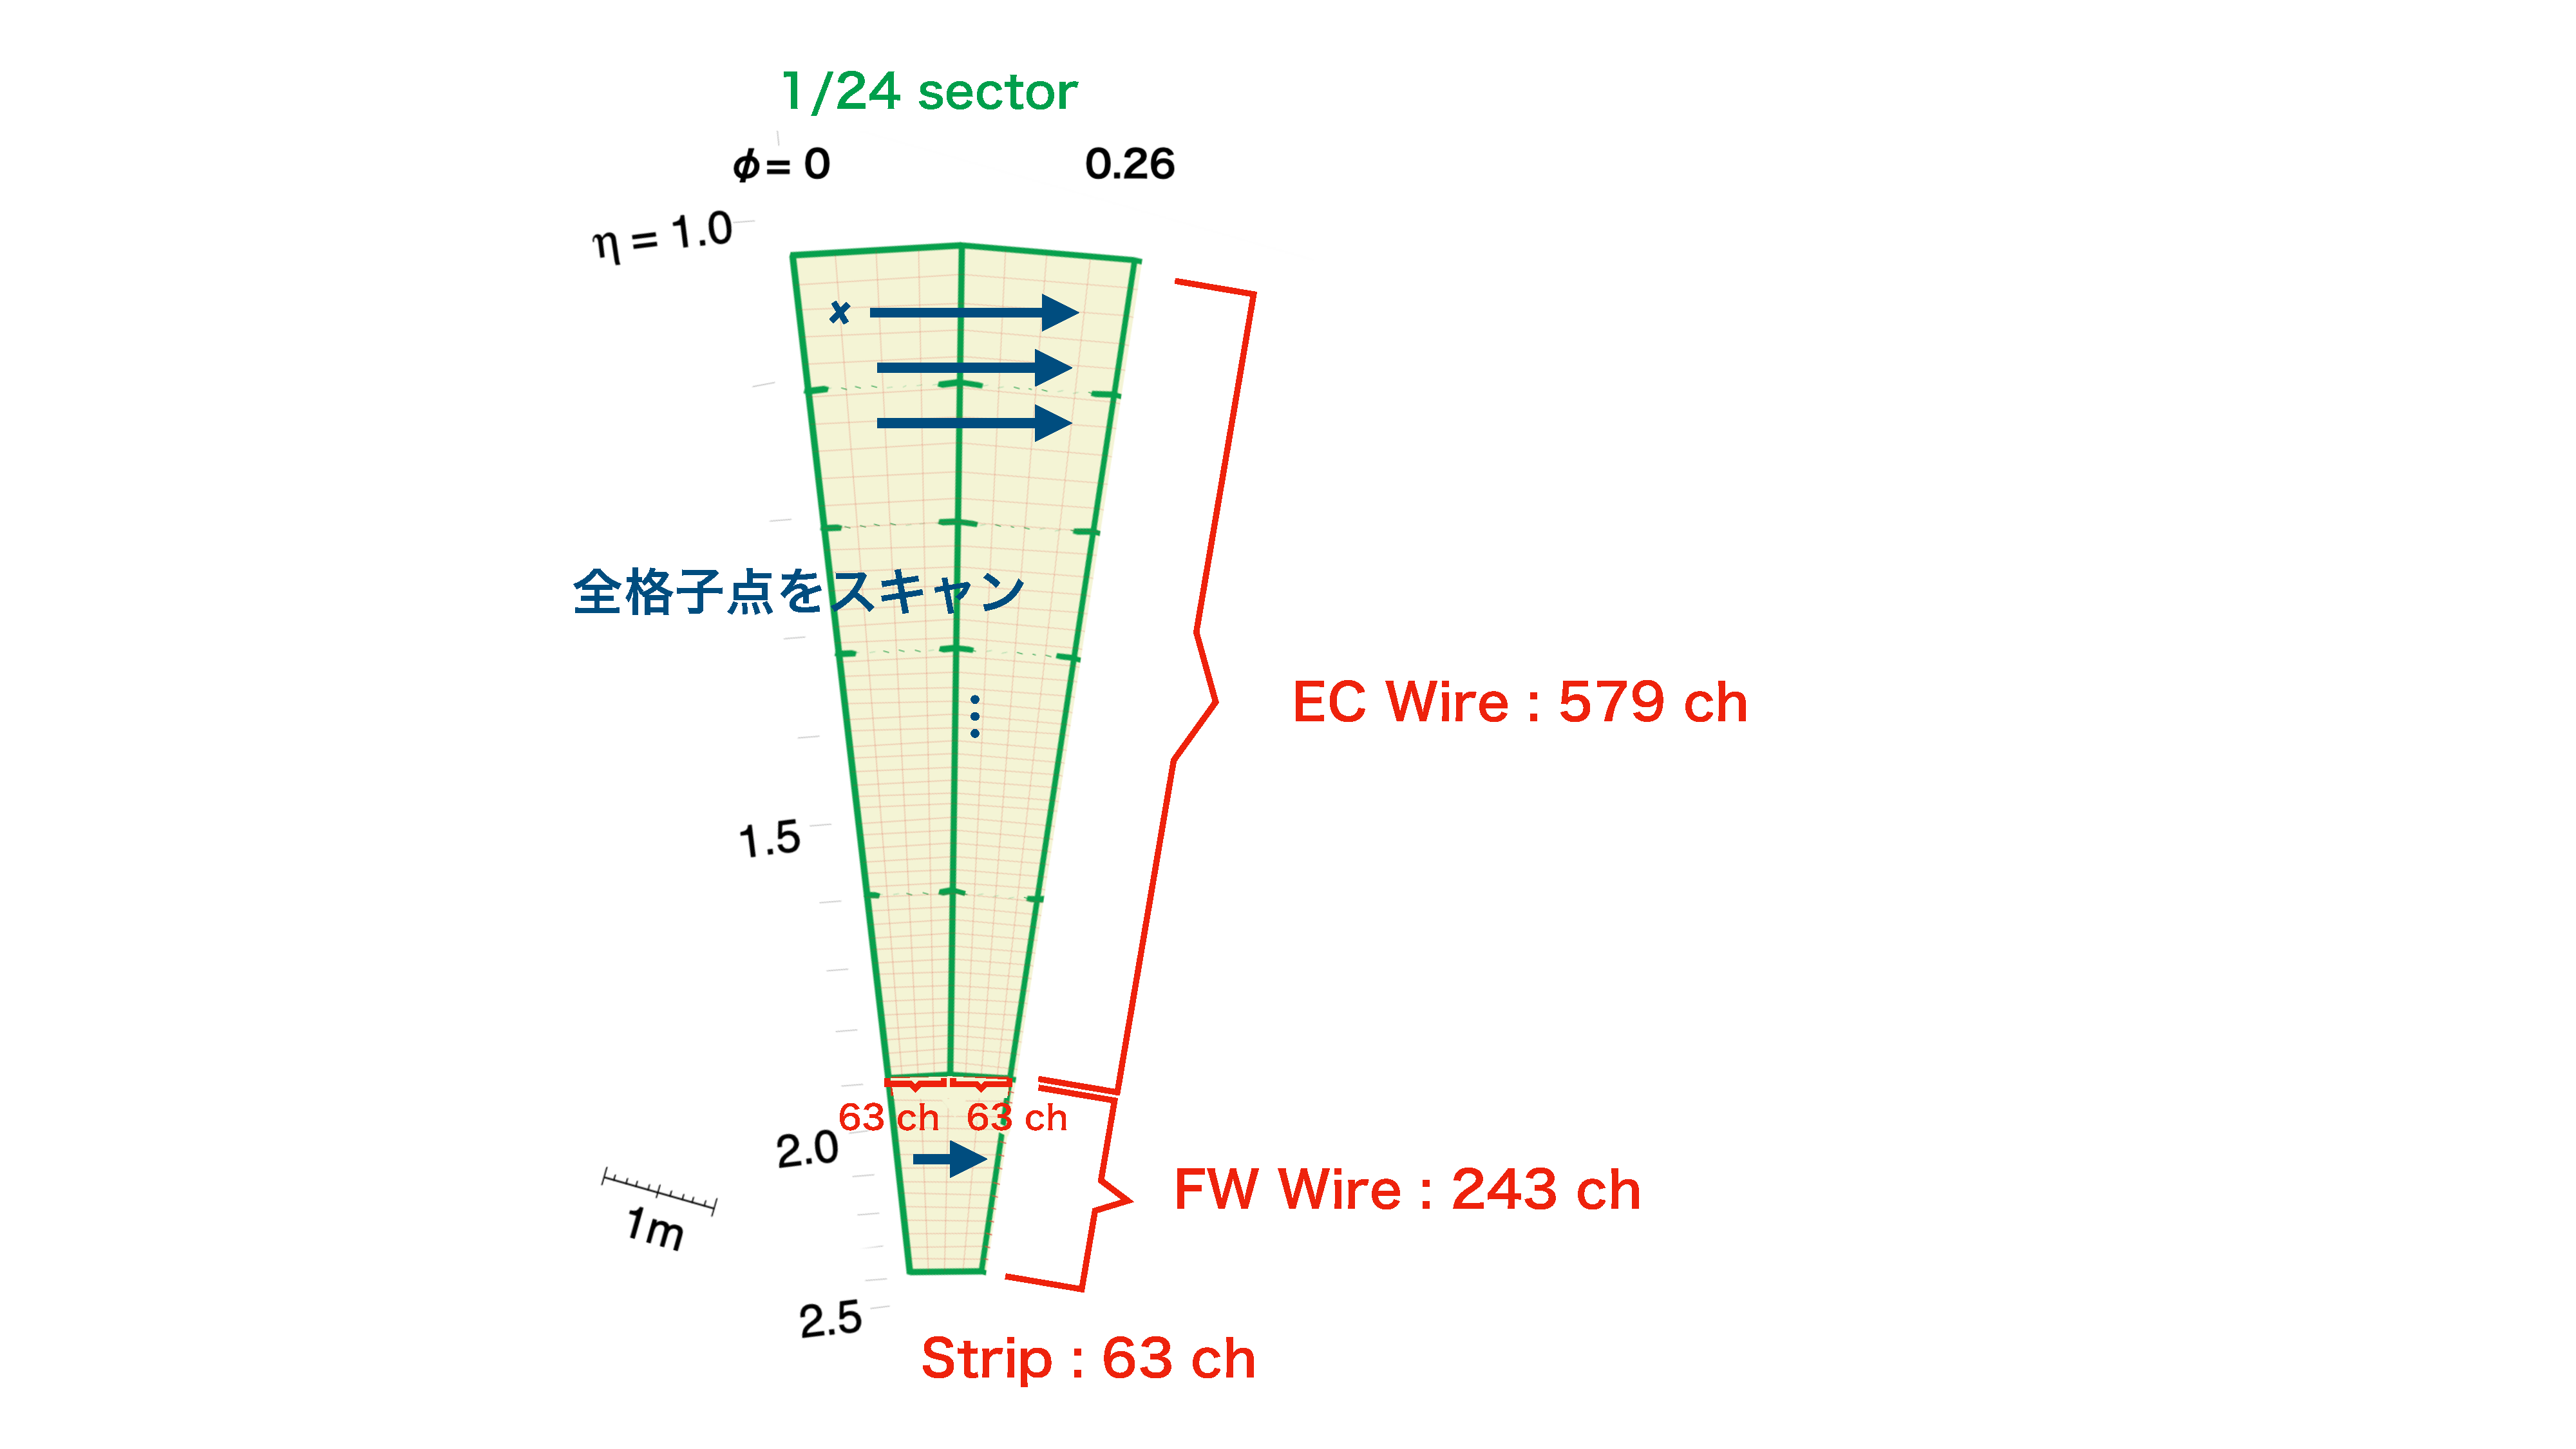
\includegraphics[width=10cm]{fig/Test/InfMomentum.pdf}
\caption[用意した無限運動量飛跡のデータセット]{用意した無限運動量飛跡のデータセット。FW、EC領域に存在する全2次元格子点に対して網羅的にテストパターンを用意。EC $\phi\,0$、$\phi\,1$領域はWireが579 個、Stripが63 個あるため合計36,477の格子点が存在する。FW領域はWireが243 個、Stripが63 個あるため合計15,309の格子点が存在する。}
\label{InfMomentum}
\end{figure}

図\ref{Inf_A_Strip}$\sim$図\ref{Inf_A_WS}に各モジュールごとの結果を示す。横軸にM3におけるStripのスタッガードID、縦軸にM3におけるWireのスタッガードIDをとる。各格子点をピボットとする無限運動量飛跡をシングルボード試験システムに投入し、飛跡再構成に成功した場合はその格子点を白色、失敗した場合は黒色で塗り潰す。飛跡再構成に成功したイベントの割合を表\ref{tab:InfMomentum}にまとめる。同様の試験をBitwiseシミュレーターで行ったところ、全てのトリガーモジュールで飛跡再構成の成功率は100 \%であった。

\begin{table}[]
    \centering
    \caption[無限運動量飛跡に対するトリガー回路の応答]{無限運動量飛跡に対する飛跡再構成の成功率}
    \label{tab:InfMomentum}
    \begin{tabular}{|c|c|c|c|}
    \hline
        & \begin{tabular}[c]{@{}c@{}}Strip Segment \\ Reconstruction\end{tabular} & \begin{tabular}[c]{@{}c@{}}Wire Segment\\ Reconstruction\end{tabular} & \begin{tabular}[c]{@{}c@{}}Wire Strip \\ Coincidence\end{tabular} \\ \hline\hline
    FW  & 100 \%                                                                  & 99.9 \%                                                               & 99.2 \%                                                           \\ \hline
    EC0 & 100 \%                                                                  & 99.7 \%                                                               & 97.0 \%                                                           \\ \hline
    EC1 & 100 \%                                                                  & 99.9 \%                                                               & 96.5 \%                                                           \\ \hline
    \end{tabular}
\end{table}

\subsubsection*{Strip Segment Reconstructionの結果}
Strip Segment Reconstructionではフォワード領域とエンドキャップ領域の全格子点に対して飛跡再構成に成功した。この結果はChannel Mapping、Strip Station Coincidence、Strip Segment Reconstruction、の論理回路実装が適切に行われたこと、作成されたLUTが抜けなく実装されていること、そしてLUTの書き込みやタイミング制御などトリガーを稼働させるのに必要なコントロール機能が正確に動作していることを示している。さらに、この結果はシングルボード試験システム自体が正確に動作していることも示唆している。MPSoCからのテストパターンを書き込むパスとトリガー回路の読み出しパスは安定して動作しており、TTC emulator、トリガー回路、読み出しパスが固定レイテンシーで制御されていることを示している。これらのコントロールおよび読み出しパスは実験本番でも使われるシステムであり、SL統合ファームウェア全体が精度良く動作していることを示している。この結果を得られるまでの過程で、本研究によって
Strip LUTのミスを発見し、修正を行った。デバッグの過程をはAppendix \ref{sec:appendix:infinite-momentum-tracks}に詳述する。

\begin{figure}
    \begin{minipage}[b]{.5\linewidth}
        \centering
        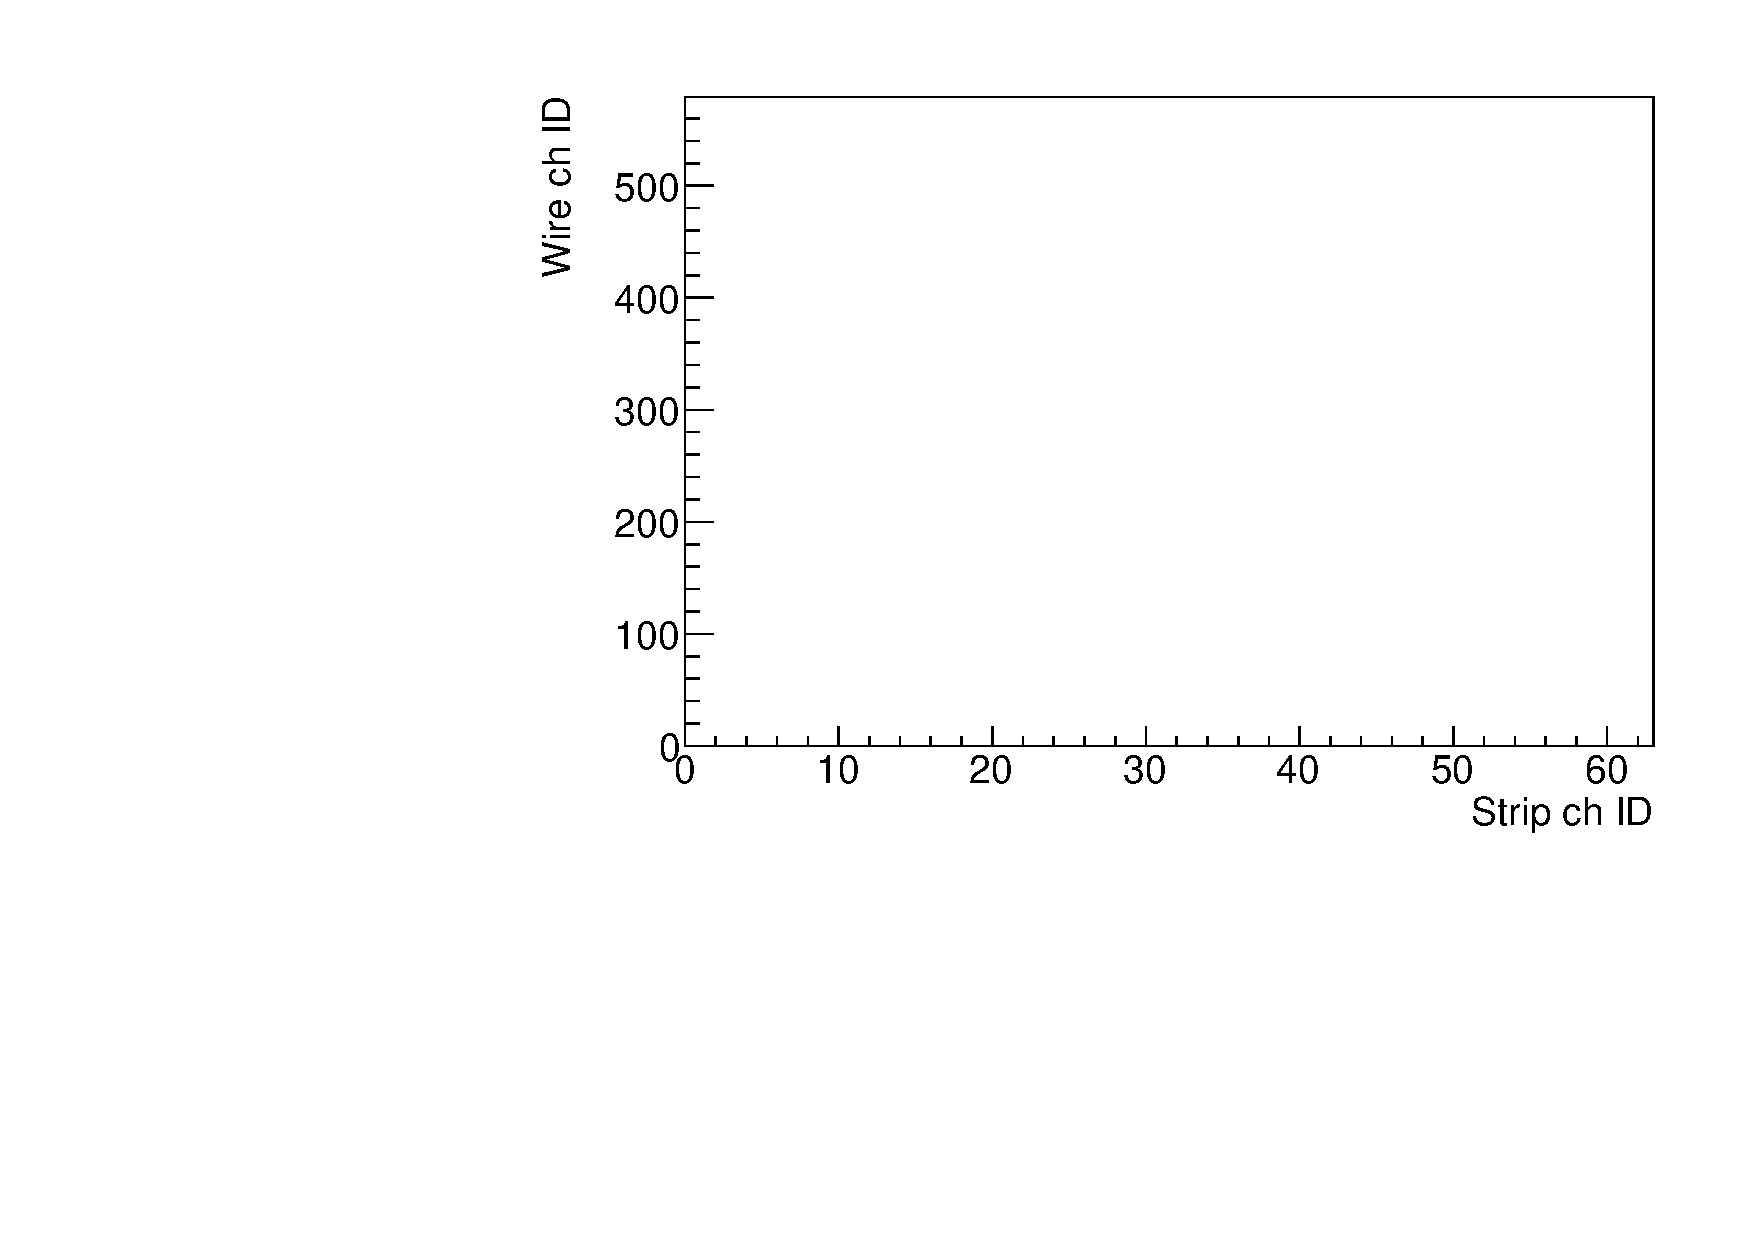
\includegraphics[height=5.6cm]{fig/Test/A_InfEC0_strip.pdf}
        \subcaption{エンドキャップ$\phi\,$0領域の結果}
    \end{minipage}
    \begin{minipage}[b]{.5\linewidth}
        \centering
        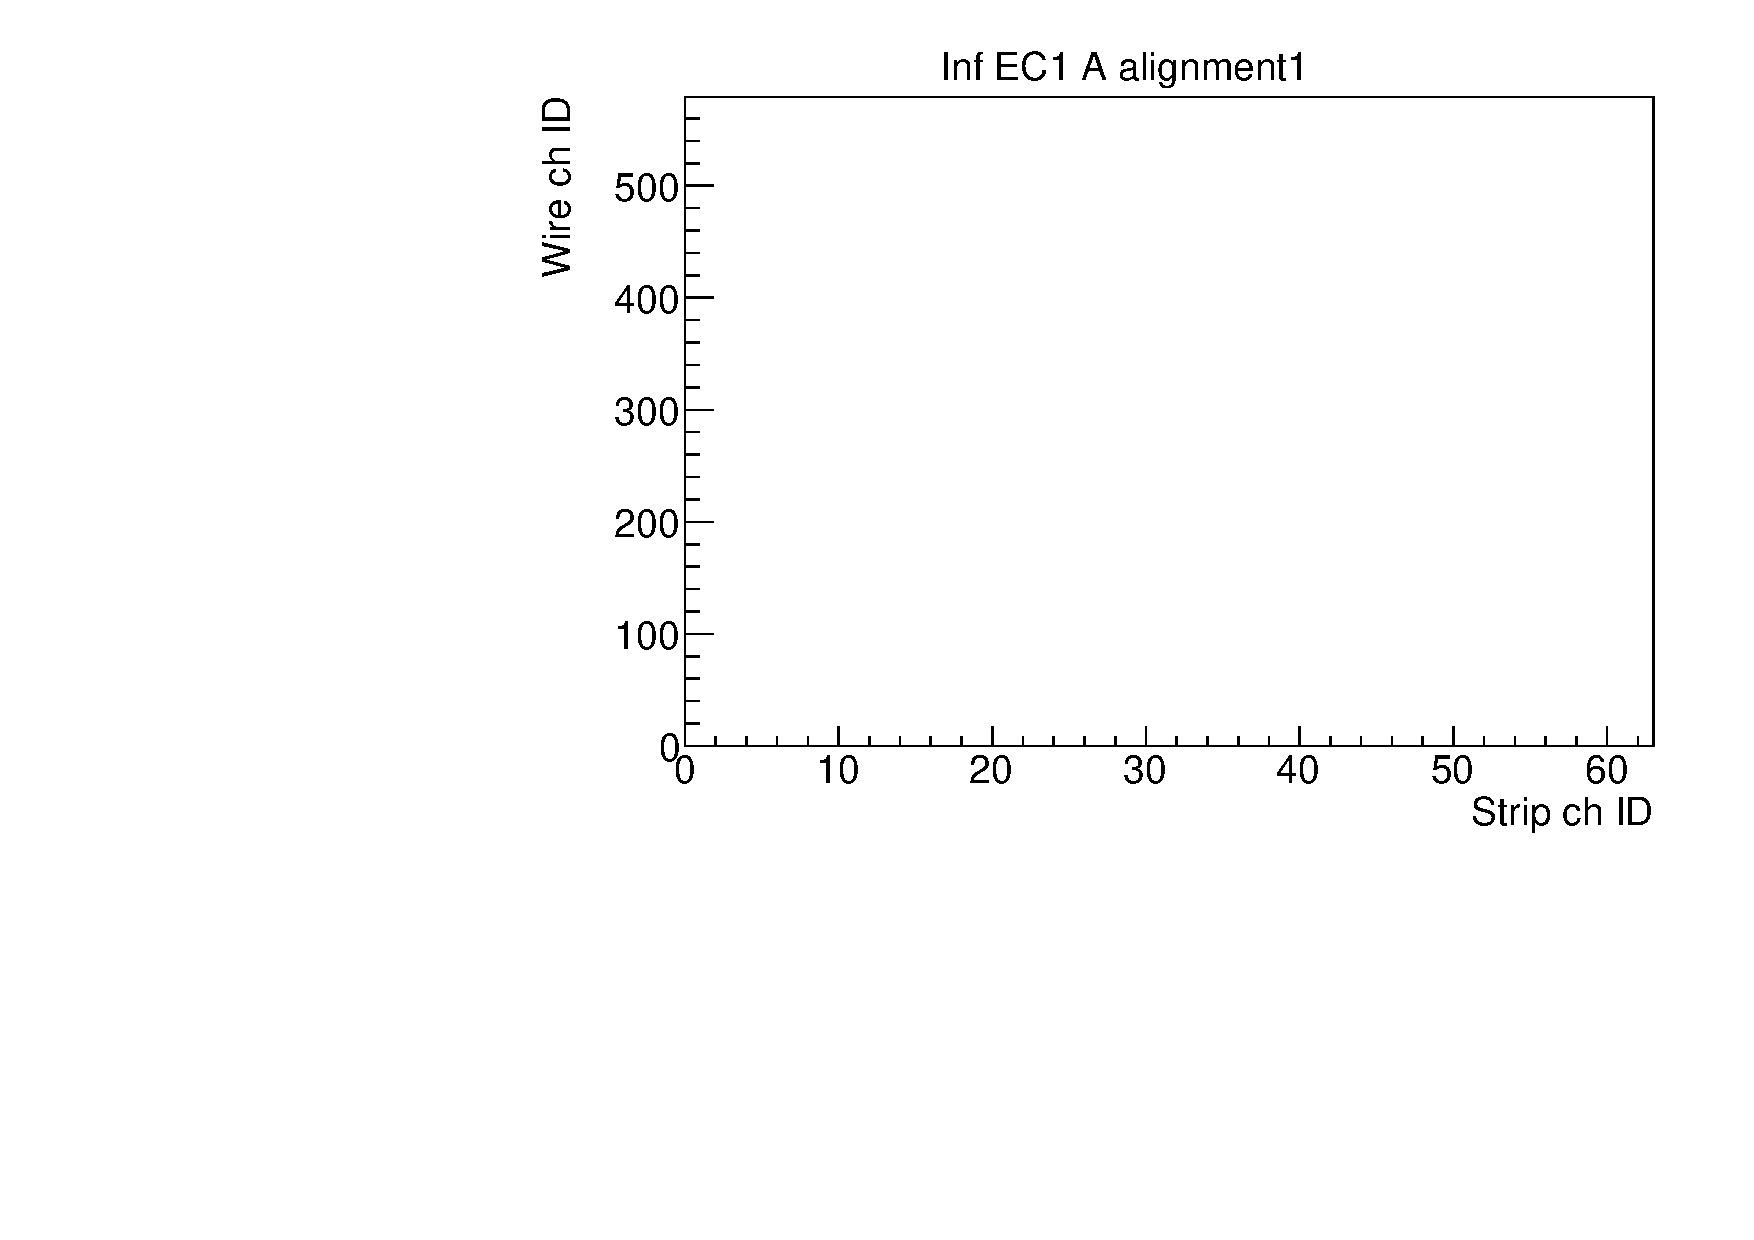
\includegraphics[height=5.6cm]{fig/Test/A_InfEC1_strip.pdf}
        \subcaption{エンドキャップ$\phi\,$1領域の結果}
    \end{minipage}\\
    \begin{minipage}[b]{\linewidth}
        \centering
        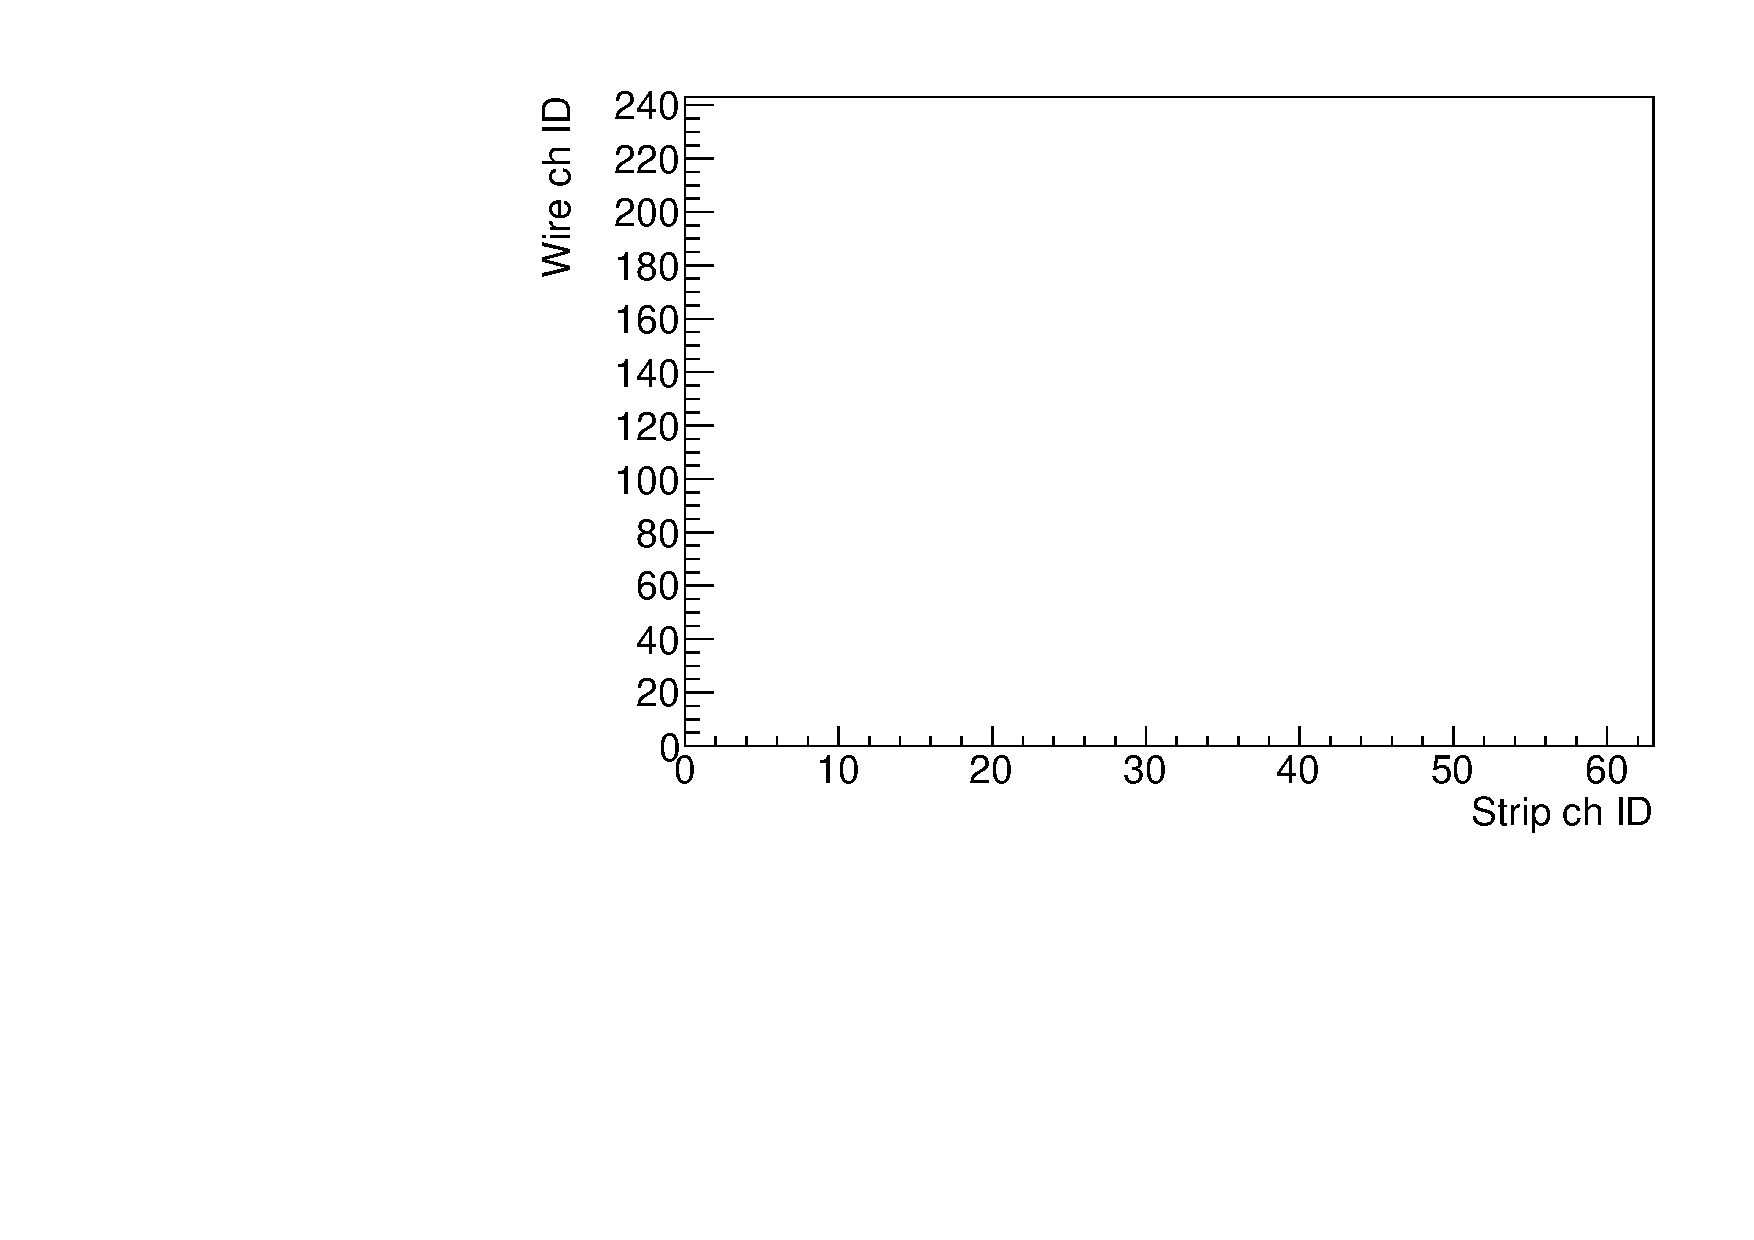
\includegraphics[height=5.6cm]{fig/Test/A_InfFW_strip.pdf}
        \subcaption{フォワード領域の結果}
    \end{minipage}
    \caption[無限運動量飛跡に対する、Strip Segment Reconstructionの応答]{無限運動量飛跡に対する、Strip Segment Reconstructionの応答。横軸にM3におけるStripのスタッガードID、縦軸にM3におけるWireのスタッガードIDをとる。各2次元格子点をピボットとする無限運動量飛跡をシングルボード試験システムに投入し、$0 \leq \Delta\phi$ のSegmentを再構成できた場合にはその格子点を白色、できなかった場合は黒色で塗り潰す。この結果は、全ての2次元格子点で飛跡再構成に成功したことを示す。}
    \label{Inf_A_Strip}
\end{figure}

\subsubsection*{Wire Segment Reconstructionの結果}
Wire Segment Reconstructionでは、フォワード領域で99.9 \% (15,287 / 15,309)、エンドキャップ$\phi\,$0領域で99.7 \% (35,370 / 36,477)、エンドキャップ$\phi\,$1領域で99.9\% (36.181 / 36.477)の飛跡再構成に成功した。一方で、全領域において特定の構造を持たない$\mathcal{O}(0.1\,\%)$のInefficiencyが観測された。\footnote{エンドキャップ$\phi\,$1領域のWire スタッガード ID $0 \sim 2$ の範囲でもInefficiencyが見られるが、これはM3とM1の$\eta$方向のカバレージの違いによるものであると理解されている。$\phi1$領域の$\eta\sim$2.0付近の領域では、M3がM1よりも広い$\eta$範囲をカバーしている。そのため、M3の代表点をピボットにして代表点を割り振ると同じ代表点をもつチャンネルでも$\eta$位置にずれが生じ、直線的な飛跡にならない。
}

このInefficiencyに関しては、Bitwiseシミュレーターでは確認されていないため、シングルボード試験システム固有の問題であると考えられる。これまでの調査の結果、飛跡再構成に失敗する格子点の位置は、データ取得のたびに変わることが判明している。失敗するイベントの割合は試験ごとに概ね一定で、Wire Segment Reconstruction では約0.1 \%である。現時点では、この問題がハードウェア上のトリガー回路自体の問題に起因するのか、それとも読み出し回路の問題に起因するのかの区別がついておらず、問題の解決には至っていない。今後、詳細な調査を進め、原因の解明と修正に努める。一方で、後述するトリガー回路の性能評価においては$\mathcal{O}(10 \%)$ 程度のInefficiencyについて議論するため、この$\mathcal{O}(0.1 \%)$程度のInefficiencyは今後の議論には影響しないと考えられる。

この結果を得られるまでの過程で、本研究によって無限運動量飛跡生成機構に問題を発見し、修正を行った。デバッグの過程をAppendix \ref{sec:appendix:infinite-momentum-tracks}に詳述する。

\begin{figure}
    \begin{minipage}[b]{.5\linewidth}
        \centering
        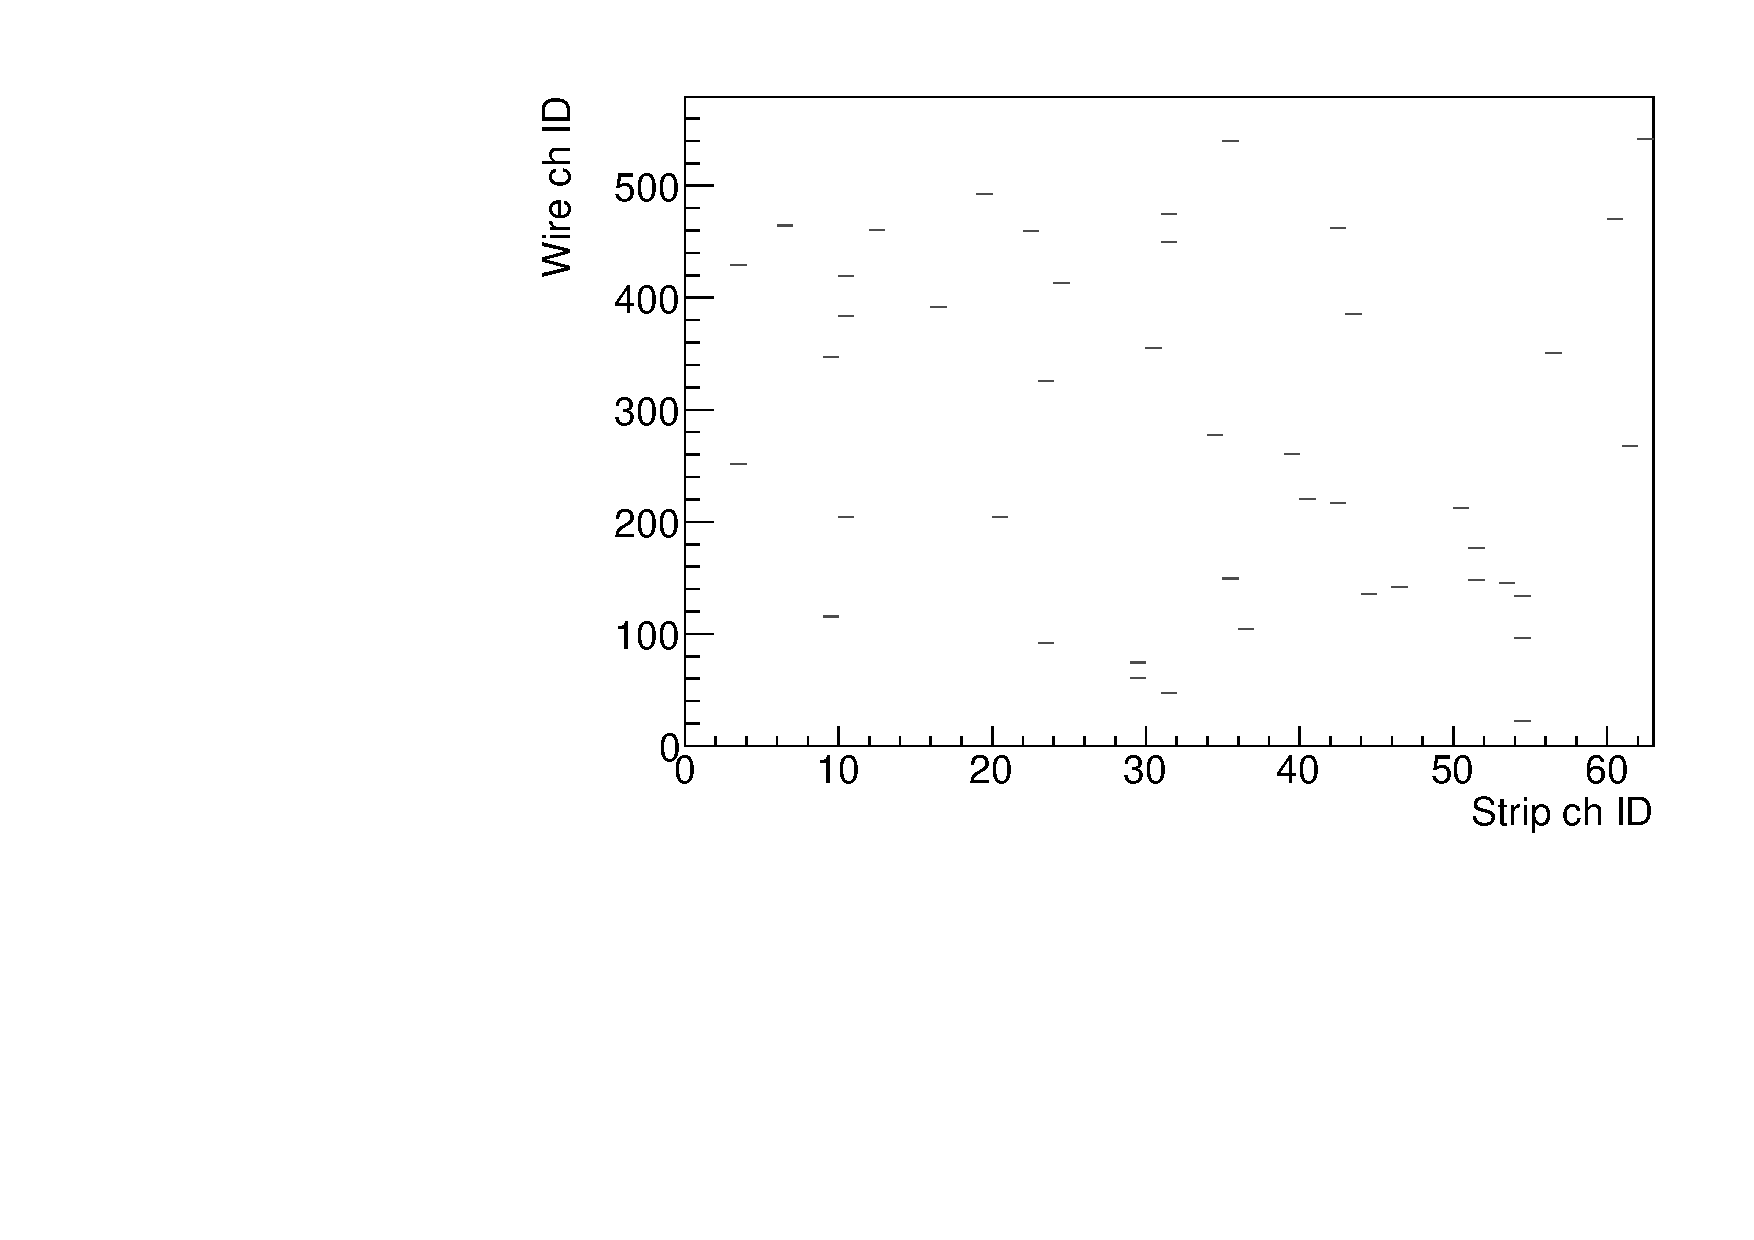
\includegraphics[height=5.6cm]{fig/Test/A_InfEC0_wire.pdf}
        \subcaption{エンドキャップ$\phi\,$0領域の結果}
    \end{minipage}
    \begin{minipage}[b]{.5\linewidth}
        \centering
        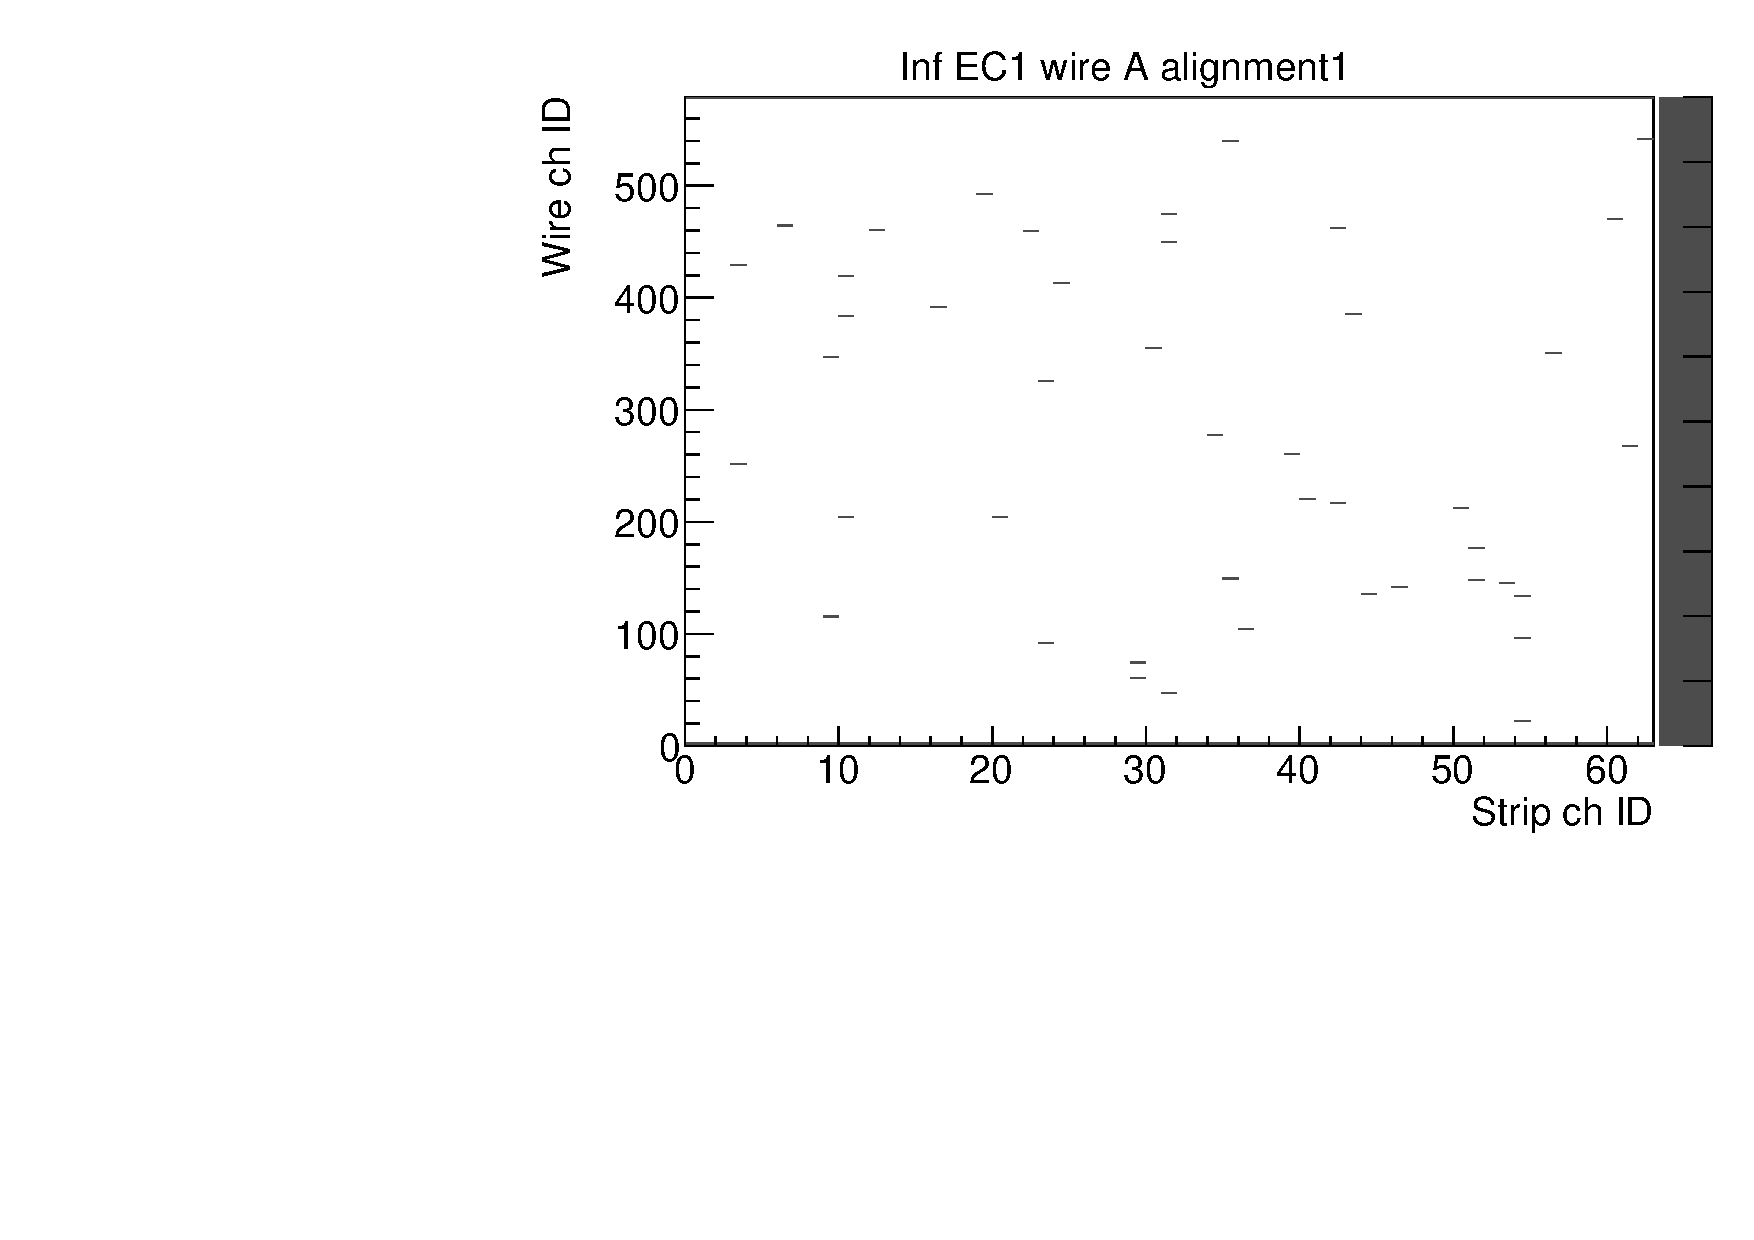
\includegraphics[height=5.6cm]{fig/Test/A_InfEC1_wire.pdf}
        \subcaption{エンドキャップ$\phi\,$1領域の結果}
    \end{minipage}\\
    \begin{minipage}[b]{\linewidth}
        \centering
        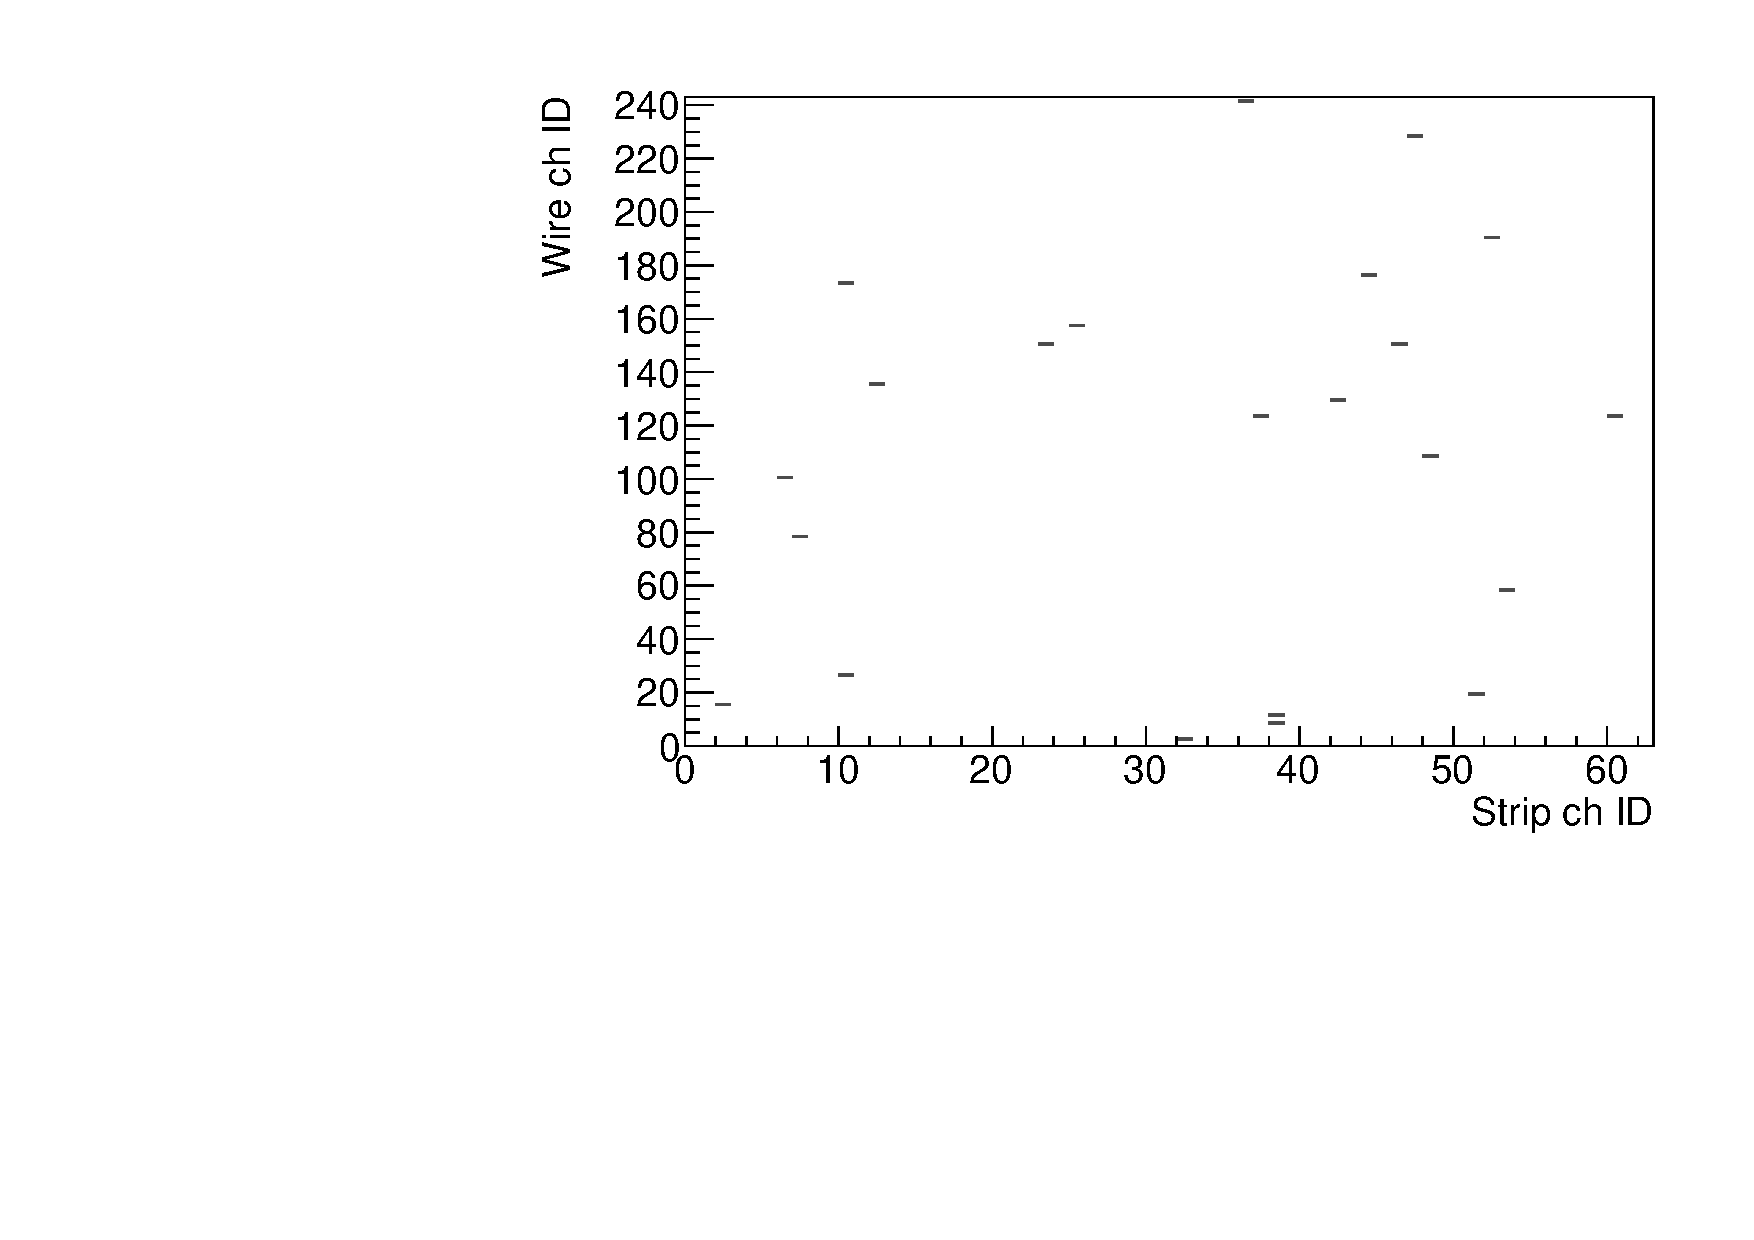
\includegraphics[height=5.6cm]{fig/Test/A_InfFW_wire.pdf}
        \subcaption{フォワード領域の結果}
    \end{minipage}
    \caption[無限運動量飛跡に対する、Wire Segment Reconstructionの応答]{無限運動量飛跡に対する、Wire Segment Reconstructionの応答。横軸にM3におけるStripのスタッガードID、縦軸にM3におけるWireのスタッガードIDをとる。各2次元格子点をピボットとする無限運動量飛跡をシングルボード試験システムに投入し、$0 \leq \Delta\theta$ のSegmentを再構成できた場合にはその格子点を白色、できなかった場合は黒色で塗り潰す。全体の$\mathcal{O}(0.1\,\%)$程度の格子点で飛跡再構成に失敗していることがわかる。}
    \label{Inf_A_Wire}
\end{figure}


\subsubsection*{Wire Strip Coincidenceの結果}
Wire Strip Coincidence では、フォワード領域で 99.6 \% (15,179 / 15,309) 、エンドキャップ$\phi\,$0領域で 97.0 \% (35,390 / 36,477) 、エンドキャップ$\phi\,$1領域で 96.5\% (35.201 / 36.477) の飛跡再構成に成功した。一方で、フォワード領域ではWire スタッガード ID 190 番に該当する飛跡が全て再構成されないことが確認された。エンドキャップ領域では、Wire スタッガード ID 410 番以降の領域で、$\phi\,0$と$\phi\,1$のどちらにも規則的な構造を持ったInefficiencyが観測された。このInefficiencyは、同様のLUTを利用しているBitwiseシミュレーターでは再現されないため、LUTの原因ではなく論理回路の問題であると考えられる。Wire Strip Coincidence ではWire スタッガード IDが419より小さい領域は32 Unit regionで処理され、大きい領域は8 Unit regionで処理される。そのため、この構造的なInefficiencyは8 Unit regionのファームウェアの問題である可能性が高い。今後VivadoシミュレーターとBitwiseシミュレーターの途中出力を比較することで、問題が発生じている箇所を特定し、論理回路の修正を進める。

\subsection{まとめ}
無限運動量飛跡を用いた試験によって、TGC BW Coincidence の 95 \% 以上の領域でトリガー回路が正常に動作していることを確認することができた。一方で、Wire Strip Coincidenceでは、トリガーロジックの論理回路実装において発生したと思われる不具合を発見することができた。このような数 \% の局所的なInefficiencyは、網羅的かつ緻密に検証を進めたからこそ見つけられたもので、従来までは統計量の観点から見つけることが困難な問題であった。任意の位置に入射するミューオン飛跡を生成できる無限運動量飛跡生成機構と、ハードウェア上で実際に動作するトリガー回路に対して、大統計量の試験を行うことができるシングルボード試験システムの真価が発揮された例である。これらの不具合を実験開始前に発見し、修正することは、高輝度LHC-ATLAS実験の運転初日から、最大パフォーマンスでのミューオントリガーを実現する上で、重要な役割を果たす。

\begin{figure}
    \begin{minipage}[b]{.5\linewidth}
        \centering
        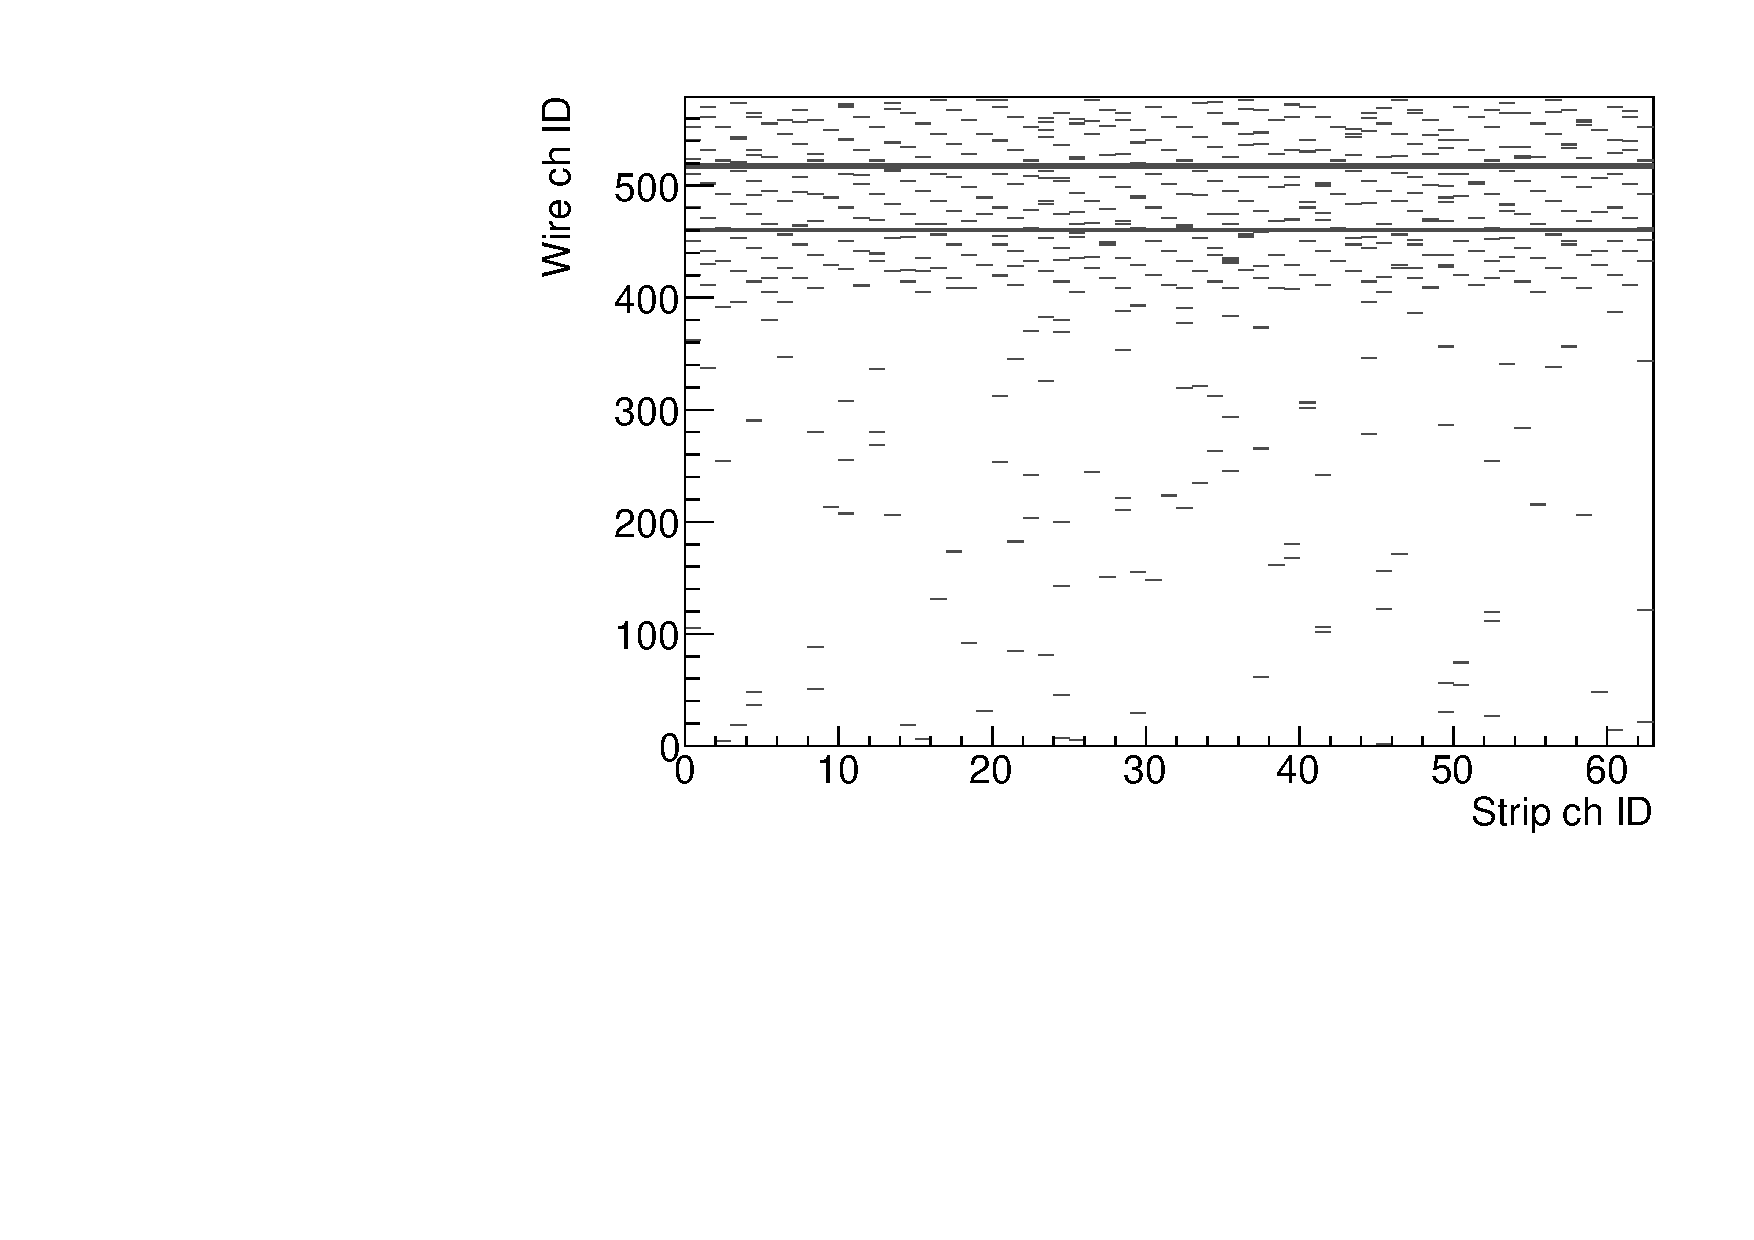
\includegraphics[height=5.6cm]{fig/Test/A_InfEC0_WS.pdf}
        \subcaption{エンドキャップ$\phi\,$0領域の結果}
    \end{minipage}
    \begin{minipage}[b]{.5\linewidth}
        \centering
        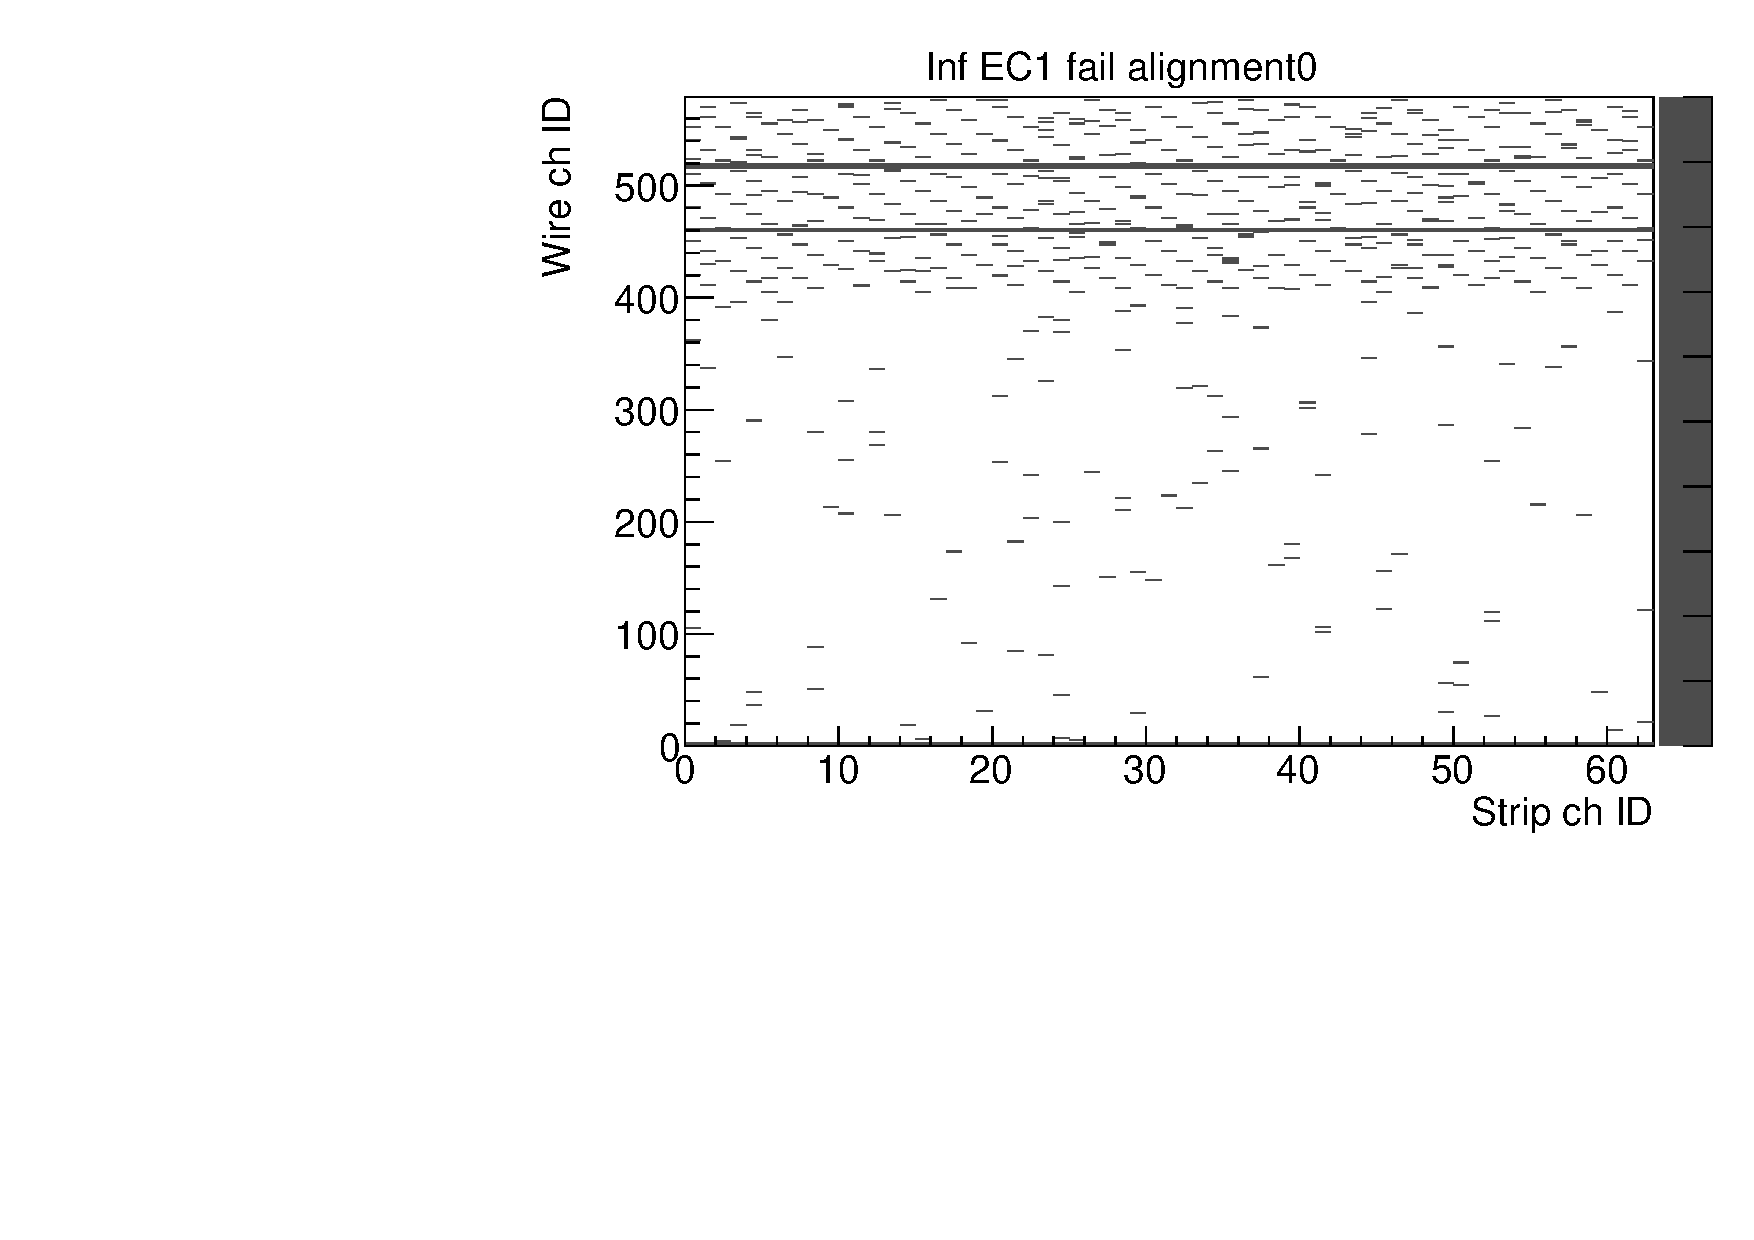
\includegraphics[height=5.6cm]{fig/Test/A_InfEC1_WS.pdf}
        \subcaption{エンドキャップ$\phi\,$1領域の結果}
    \end{minipage}\\
    \begin{minipage}[b]{\linewidth}
        \centering
        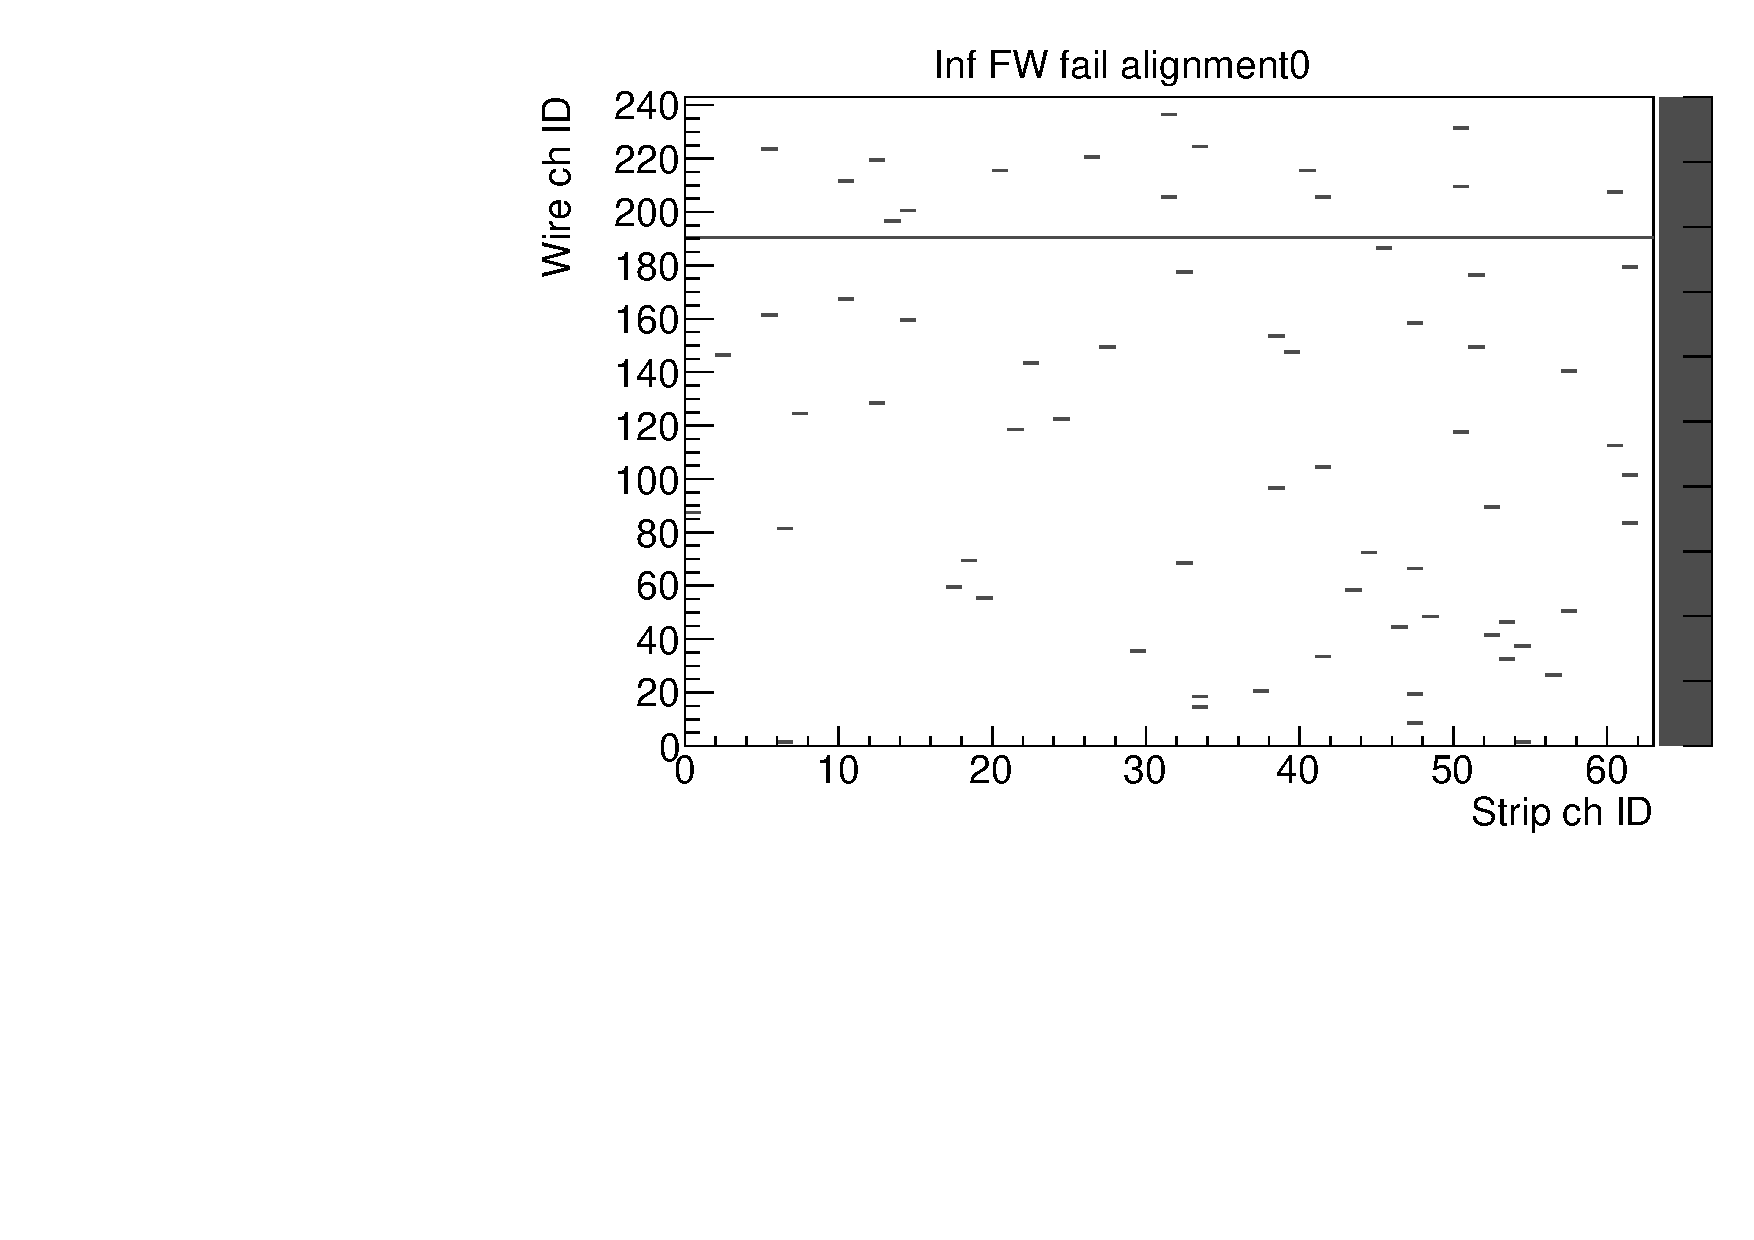
\includegraphics[height=5.6cm]{fig/Test/A_InfFW_WS.pdf}
        \subcaption{フォワード領域の結果}
    \end{minipage}
    \caption[無限運動量飛跡に対する、Wire Strip Coincidence の応答]{無限運動量飛跡に対する、Wire Strip Coincidence の応答。横軸にM3におけるStripのスタッガードID、縦軸にM3におけるWireのスタッガードIDをとる。各2次元格子点をピボットとする無限運動量飛跡をシングルボード試験システムに投入し、$0\,\mathrm{GeV} < p_\mathrm{T}$ のSegmentを再構成できた場合にはその格子点を白色、できなかった場合は黒色で塗り潰す。Forward領域ではWire スタッガード ID 190番に該当するイベントが全て再構成に失敗している。Endcap 領域ではWire スタッガード ID 410 番以降の領域で$\phi0$と$\phi1$のどちらにも規則的な構造を持ったInefficiencyが見られる。}
    \label{Inf_A_WS}
\end{figure}

\section{シミュレーションデータを用いたトリガー回路の性能評価}
\label{sec_SingleMuon}

本節では、シングルミューオンモンテカルロデータを用いたトリガー性能評価試験について述べる。シングルミューオンイベントとは、1本のミューオンが衝突点から検出器に入射する過程をエミュレートしたもので、ミューオンがTGC検出器を素通りする事象、多重散乱により飛跡が曲げられる事象、制動放射や電磁シャワーによってTGC検出器に複数のヒットが発生する事象など、実際に起こりうる物理過程を考慮したものになっている。そのためこのイベントセットを利用することで、現実的なトリガー性能を評価することができる。また、シミュレーションデータではTruth情報が含まれているため、有限の運動量をもつミューオンイベントに対して適切な\pt 判定を下すことができるいるか、などより詳細に論理回路の検証を行うことができる。

用意したデータセットの概要を表\ref{tab:SingleMuon}にまとめる。パイルアップは含まれておらず、\pt は0 GeVから50 GeV、$\eta$、$\phi$はTGC検出器がカバーする全領域に対して満遍なく用意した。また、本試験ではトリガー回路自体の性能に焦点を当てた検証を行うため、M1、M2、M3の各ステーションに少なくても1つのヒットがあることを要求している。これにより、多重散乱などで飛跡が大きく曲げられ、TGC検出器に入射しなかったイベントなどを除外している。

\begin{table}[]
    \centering
    \caption[用意したシングルミューオンモンテカルロデータの概要]{用意したシングルミューオンモンテカルロデータの概要}
    \label{tab:SingleMuon}
    \begin{tabular}{|c|c|}
    \hline
    Parameter        &                                                                                              \\ \hline
    $p_{\mathrm{T}}$ & $ 0 \, < \, p_{\mathrm{T}}\, < 50$ GeV flat                                                  \\ \hline
    $\eta$           & 1.06 \textless |$\eta$| \textless 2.4 flat                                                   \\ \hline
    $\phi$           & 0 \textless{} $\phi$ \textless 2$\pi$ flat                                      \\ \hline
    イベント数            & 500,000                                                                                      \\ \hline
    イベントカット          & \begin{tabular}[c]{@{}c@{}}1つのトリガーセクター内のM1、M2、M3各ステーションに\\ それぞれ1つ以上のヒットがあることを要求\end{tabular} \\ \hline
    \end{tabular}
\end{table}

\subsubsection*{Strip Segment Reconstructionのトリガー効率}
この試験では \pt  が十分に大きい事象に対するトリガー応答を確認することを目的とし、Truth \pt $\,$20 GeV 以上のミューオンに対する検出効率を評価する。Efficiencyは式\ref{eq:Strip_Efficiency}のように定義する。

\begin{equation}
    \mathrm {Efficiency} = \frac{\mathrm{Strip\,Segment \,Reconstruction\,で0\leq\Delta\phi\,を再構成できたイベント数}}{\mathrm{Truth\,pt \,20 \,GeV以上のイベント数}}
    \label{eq:Strip_Efficiency}
\end{equation}

Strip Segment Reconstructionの検出効率の$\eta$および$\phi$依存性を図\ref{SM_A_strip}に示す。黒色の点はSL実機の出力結果、赤色の点はBitwise シミュレーターの出力結果を表している。全領域での平均トリガー検出効率は 97.4 \%であり、先行研究\cite{mt_mino}の結果と矛盾のない結果が得られた。また、Strip Segment Reconstructionでは実機とBitwiseシミュレーターの結果が多くの領域で一致している。これはBitwiseシミュレーターが論理回路のロジックを極めて正確に再現できていることを示している。しかし、2 < $\eta$のフォワード領域の、特に1/24セクターの境界領域 (トリガー回路はTGC BWの1/24領域ごとに独立した回路になっている。$\phi$方向に2$\pi$ / 24 = 0.26 おきに1/24チェンバーの境界が存在する。) で、両者の出力に違いが生じている。原理的にはこの2つの出力は完全に一致するべきものであり、この差異はBitwiseシミュレーターとファームウェアで1/24領域の取扱い方に、わずかな違いが生じていることを示している。今後、両者のロジックを精密に比較し、出力の不一致を解消していく。

一方、Bitwiseシミュレーターの出力がSLの出力と一致したとしても、この領域では15 \%程度のInefficiencyが生じている。このイベントセットでは事前に3つのステーションにヒットがあることを要求しているため、原理的にはチェンバー境界であってもEfficiencyが下がることはない。ファームウェア自体の論理回路実装のミス、もしくはLUTの不具合である可能性が高い。
今後これに関する調査も進め、原因を特定し修正を行う。

\begin{figure}
\begin{minipage}[b]{\linewidth}
\centering
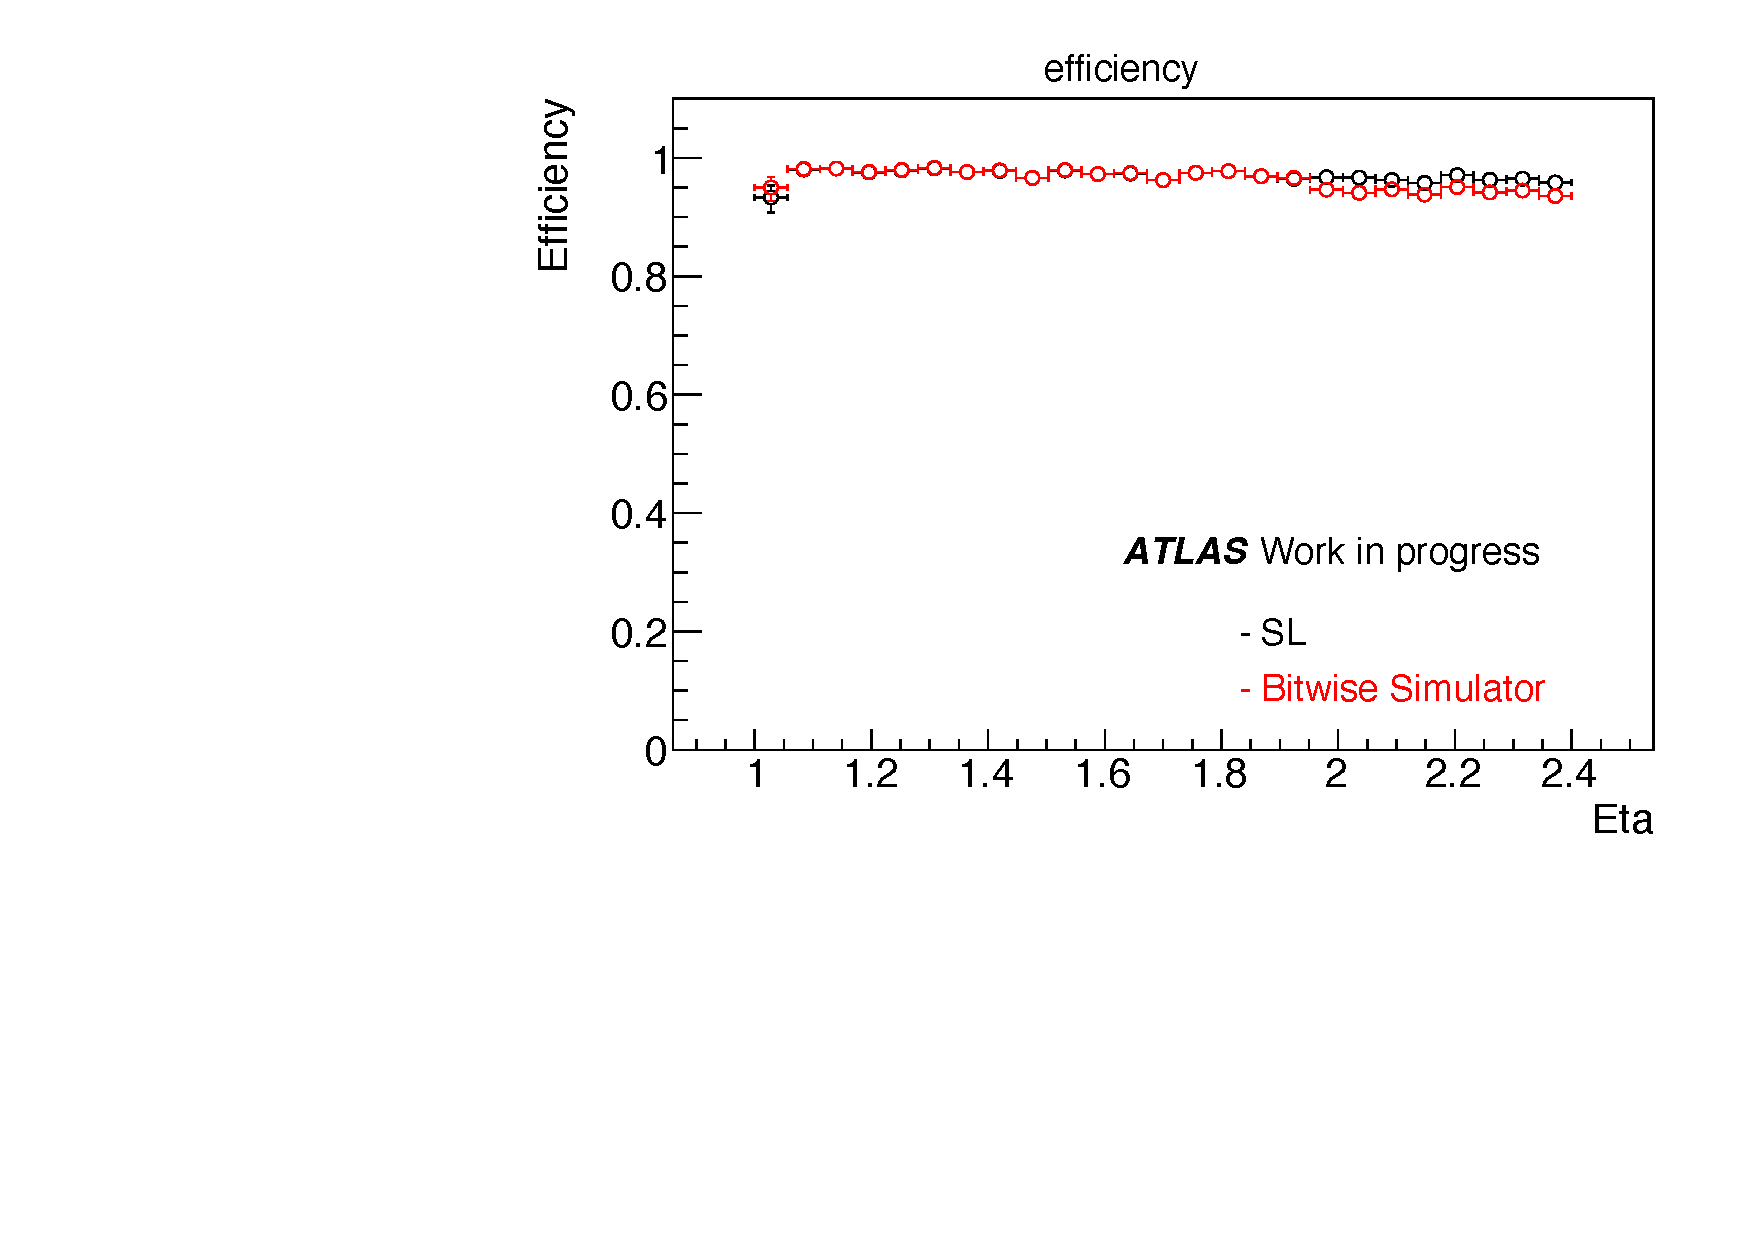
\includegraphics[height=10cm]{fig/Test/A_SM_strip_eta.pdf}
\subcaption{Strip Segment Reconstructino 検出効率の$\eta$依存性}
\end{minipage}\\
\begin{minipage}[b]{\linewidth}
\centering
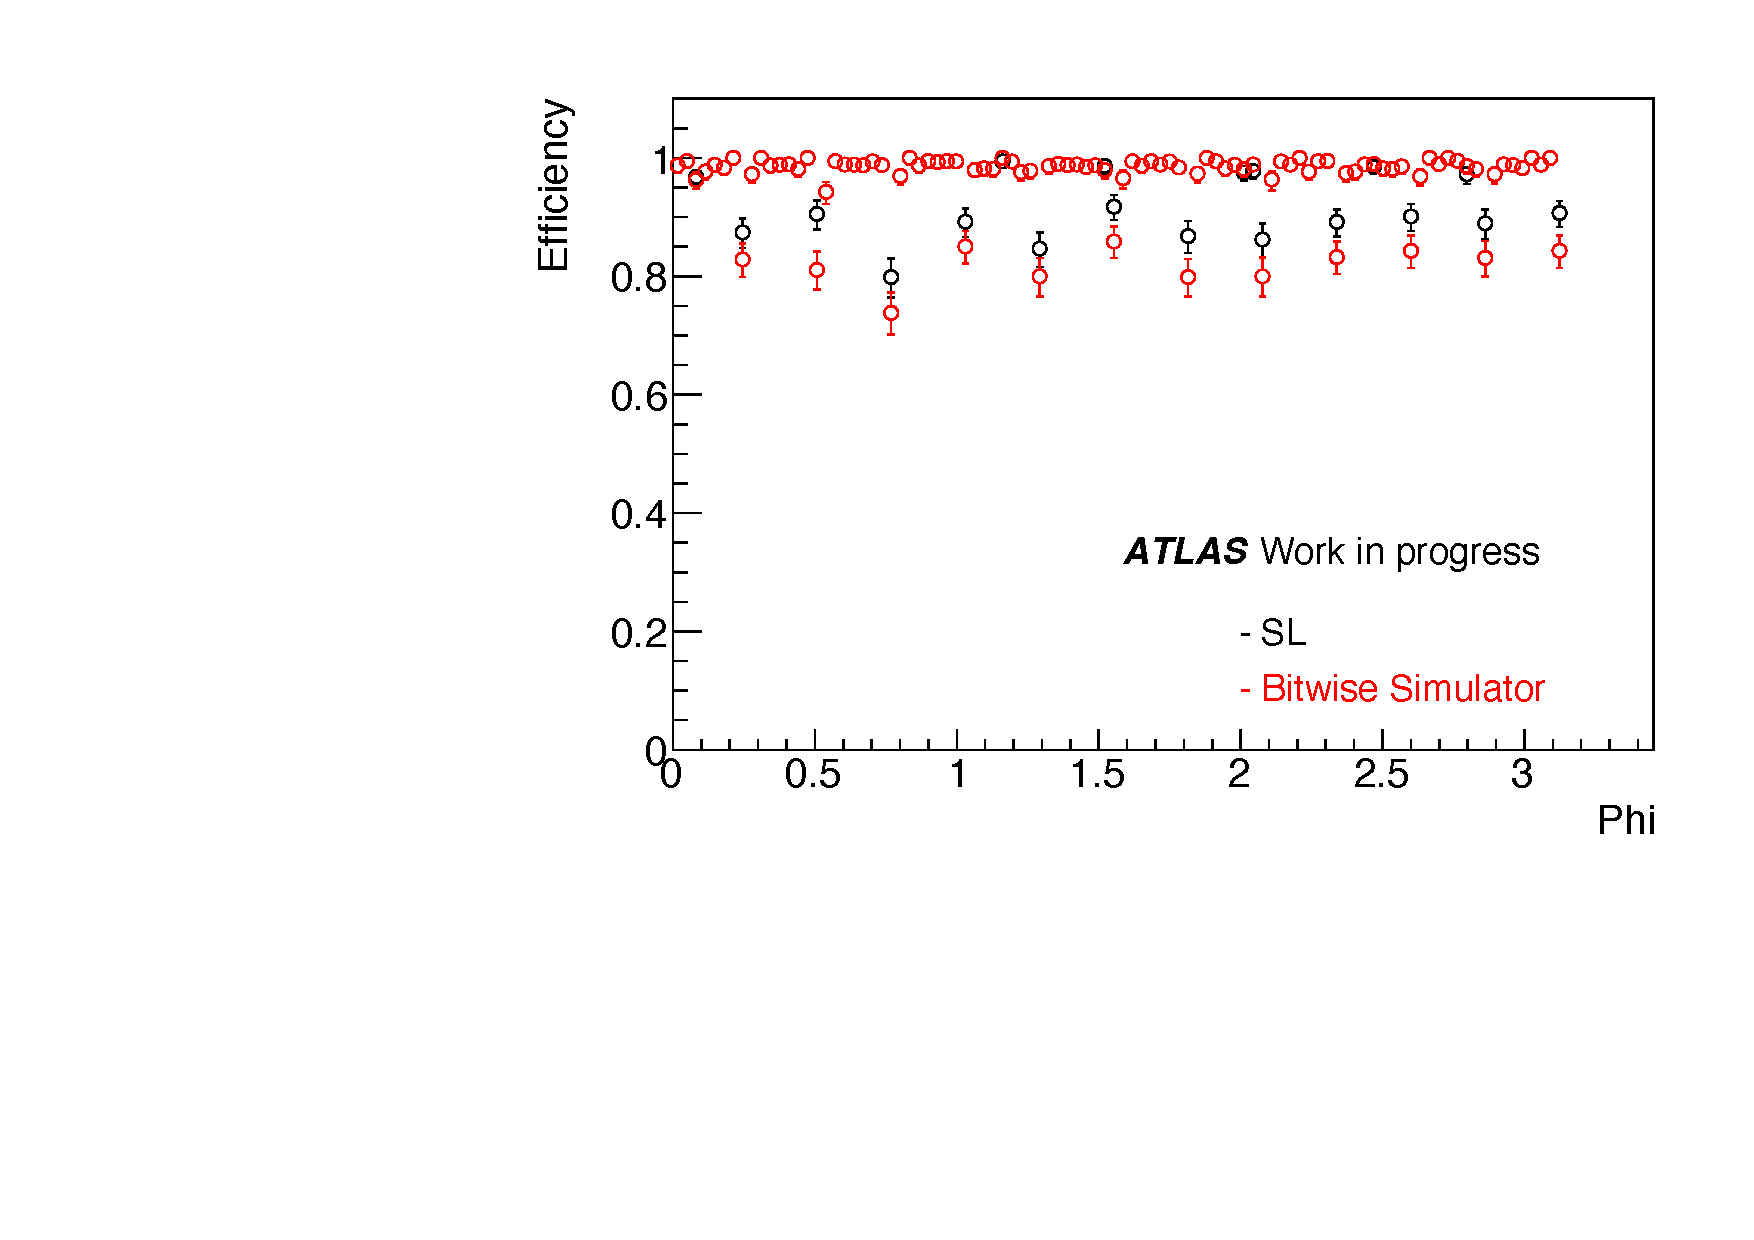
\includegraphics[height=10cm]{fig/Test/A_SM_strip_phi.pdf}
\subcaption{Strip Segment Reconstructino 検出効率の$\phi$依存性}
\end{minipage}%
\caption[Strip Segment Reconstructionの検出効率]{Strip Segment Reconstructionの検出効率。黒色のプロットが実機出力、赤色のプロットがBitwiseシミュレータの出力を表す。全領域のトリガー検出効率は97.4 \%であり、先行研究と矛盾のない結果が得られた。トリガー効率の$\phi$依存性に着目すると、シングルボード試験システムでもBitiwiseシミュレーターでも、チェンバー境界領域で10 \%程度のInefficiencyが見られる。また、フォワード領域の、特にチェンバー境界領域で実機とBitwiseシミュレーターで出力が一致していないイベントが数 \%程度存在している。}
\label{SM_A_strip}
\end{figure}



\subsubsection{Wire Segment Reconstructionのトリガー効率}
\par
Stripの場合と同様に、Efficiencyは式\ref{eq:Wire_Efficiency}のように定義する。

\begin{equation}
    \mathrm {Efficiency} = \frac{\mathrm{Wire\,Segment \,Reconstruction\,で0\leq\Delta\theta\,を再構成できたイベント数}}{\mathrm{Truth\,pt \,20 \,GeV以上のイベント数}}
    \label{eq:Wire_Efficiency}
\end{equation}


Wire Segment Reconstructionの検出効率の$\eta$および$\phi$依存性を図\ref{SM_A_strip}に示す。全領域での平均トリガー効率は 96.3 \%であり、先行研究(\ref{Vivado_Wire_Efficiency})と矛盾しない結果が得られた。

トリガー効率の$\eta$依存性に着目すると、$\eta \sim 1.4$ 付近で約5 \%のInefficiencyが見られる。このInefficiencyに対してBitwiseシミュレーターを用いた調査したところ、Channel Mapping、Wire Station Coincidence、およびWire Segment ReconstructionのAddress Specifierまでは期待通り動作していることが確認された。一方、Segment ExtractorでLUTにアクセスした結果、中身がNULLであったことがわかっている。今後はLUTの修正を行い、この領域のInefficiencyを改善する。

\begin{figure}
    \begin{minipage}[b]{\linewidth}
    \centering
    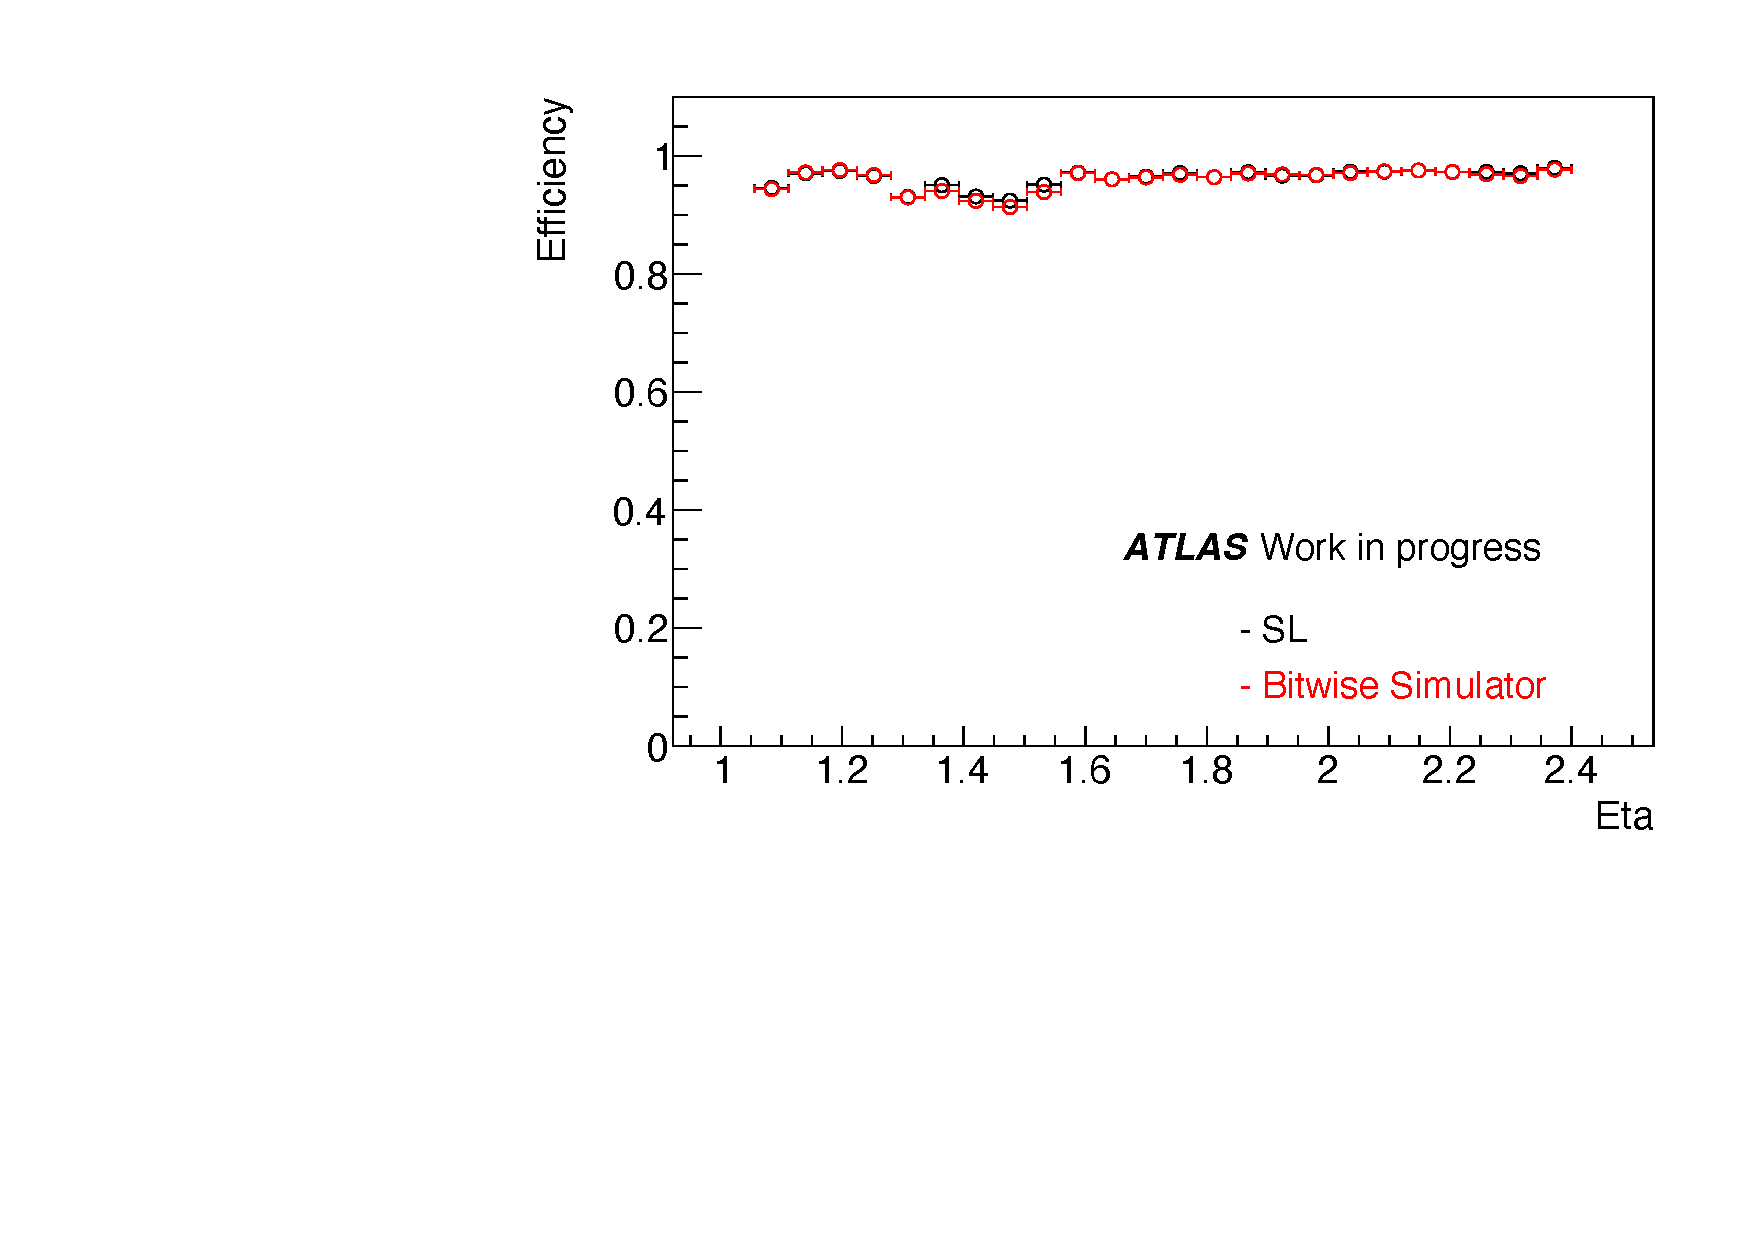
\includegraphics[height=10cm]{fig/Test/A_SM_wire_eta.pdf}
    \subcaption{Wire Segment Reconstructino 検出効率の$\eta$依存性}
    \end{minipage}\\
    \begin{minipage}[b]{\linewidth}
    \centering
    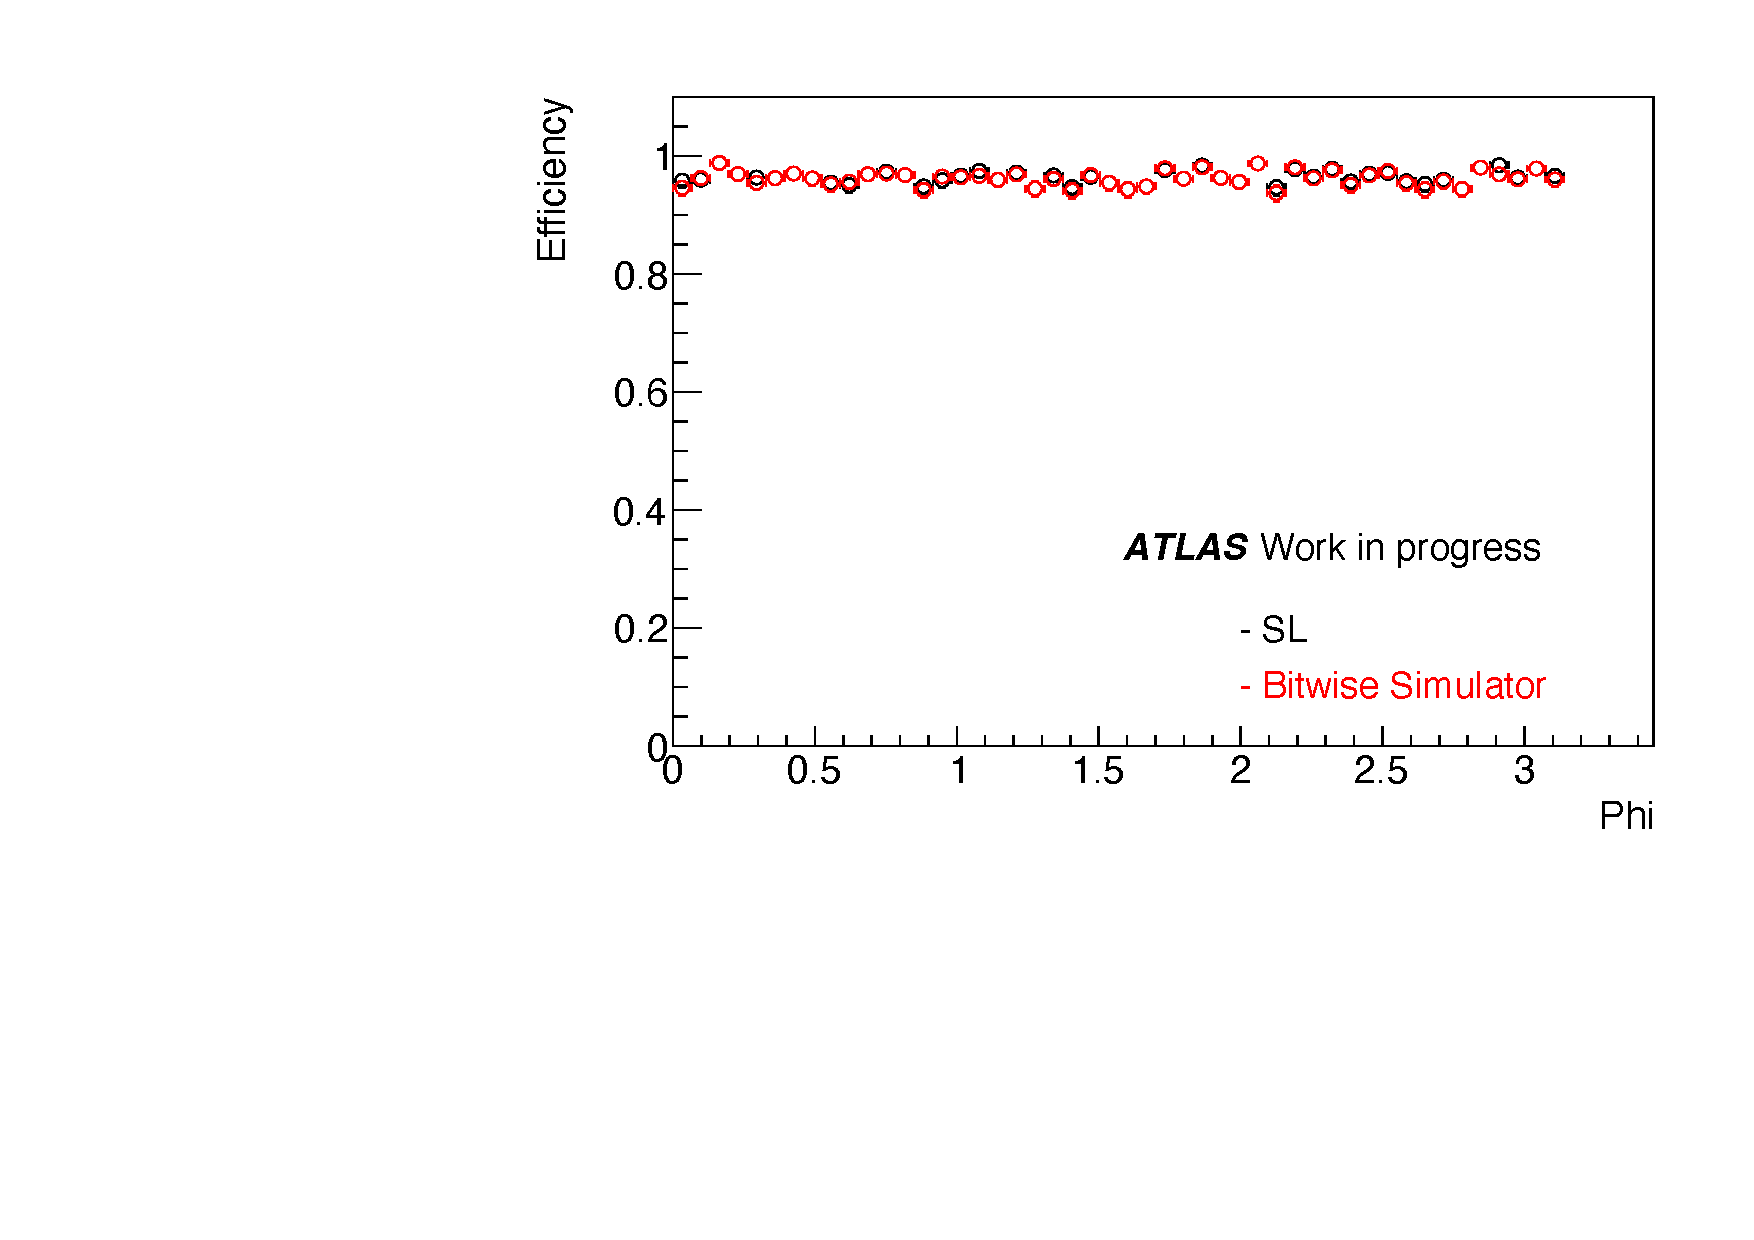
\includegraphics[height=10cm]{fig/Test/A_SM_wire_phi.pdf}
    \subcaption{Wire Segment Reconstructino 検出効率の$\phi$依存性}
    \end{minipage}%
    \caption[Wire Segment Reconstructionの検出効率]{Wire Segment Reconstructionの検出効率。黒色のプロットが実機出力、赤色のプロットがBitwiseシミュレータの出力を表す。全領域のトリガー検出効率は96.3 \%であり、先行研究と矛盾のない結果が得られた。トリガー効率の$\phi$依存性に着目すると、$\eta\sim1.4$付近で5 \%のInefficiencyが見られる。}
    \label{SM_A_Wire}
\end{figure}

\subsubsection{Wire Strip Coincidenceのトリガー効率}
Wire Strip Coincidenceは無限運動量飛跡を用いた試験で既にエンドキャップ領域に不具合が確認されているため、フォワード領域に限定して議論を進める。またStripの試験で明らかになった1/24セクター境界領域 (1/24セクターの両端から$\phi$方向に1割の領域) の不具合は、Wire Strip CoincidenceのInefficiencyにも直結するため、本試験ではこの領域も除外する。ここではEfficiencyを式\ref{eq:WS_Efficiency}のように定義する。

\begin{equation}
    \mathrm {Efficiency} = \frac{\mathrm{Wire\,Strip\, Coincidenceで\,p_\mathrm{T} \,20\,GeV以上と判定されたイベント数}}{\mathrm{Truth\,p_\mathrm{T}\,20 \,GeV以上のイベント数}}
    \label{eq:WS_Efficiency}
\end{equation}

図\ref{SM_A_WS}にWire Strip Coincidenceのフォワード領域での検出効率の$\eta$依存性及び$\phi$依存性を示す。平均のトリガー効率は 93.5 \%であり、先行研究\cite{mt_kawamoto}の結果と矛盾のない結果が得られた。トリガー効率の$\eta$依存性に着目すると、$\eta\sim1.95、2.2$付近で5 \%のInefficiencyが見られる。この領域は実機の出力とBitwiseシミュレーターの出力で違いが大きく見られる領域でもあるため、Bitwiseシミュレーターと実機の出力を詳細に比較することで、まずはこの差の解消に努める。

\begin{figure}
    \begin{minipage}[b]{\linewidth}
    \centering
    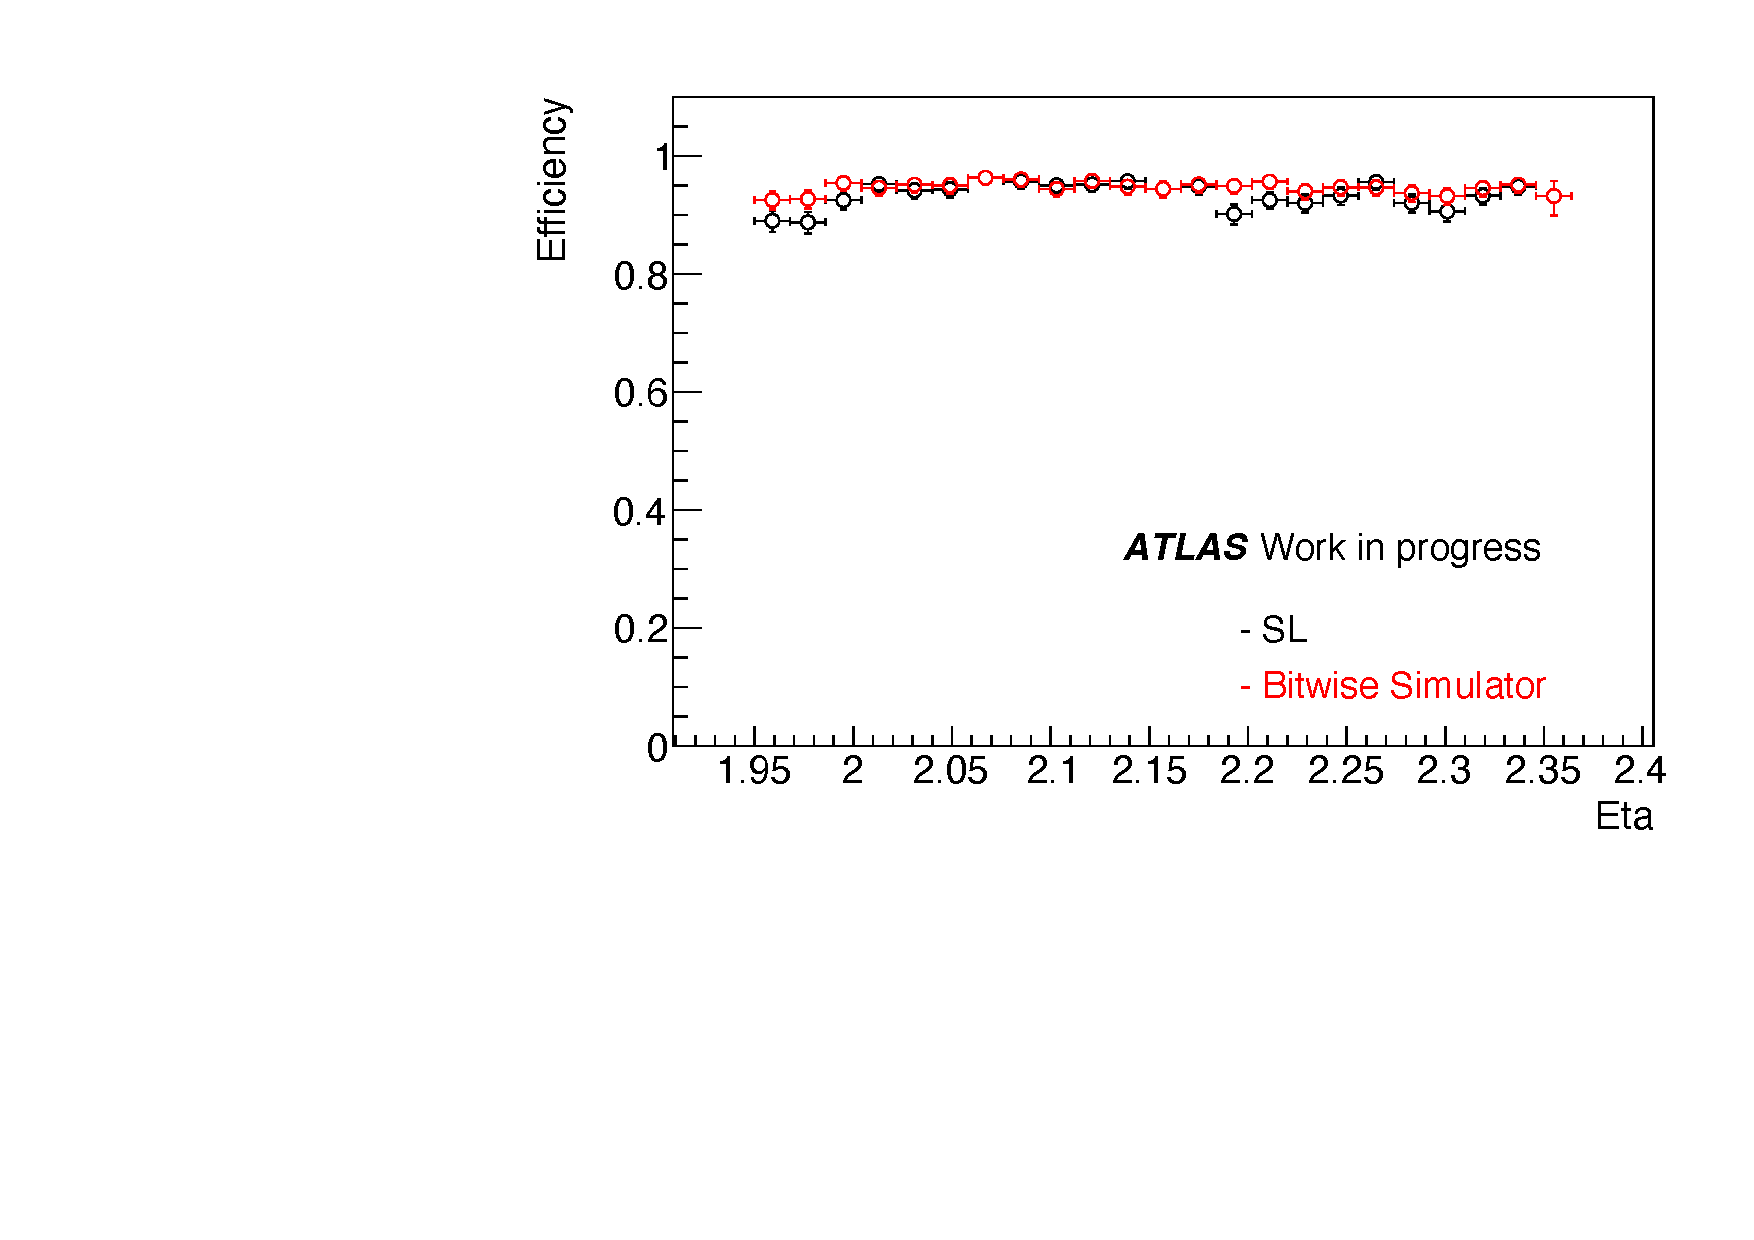
\includegraphics[height=10cm]{fig/Test/A_SM_ws_eta.pdf}
    \subcaption{Wire Strip Coincidence 検出効率の$\eta$依存性}
    \end{minipage}\\
    \begin{minipage}[b]{\linewidth}
    \centering
    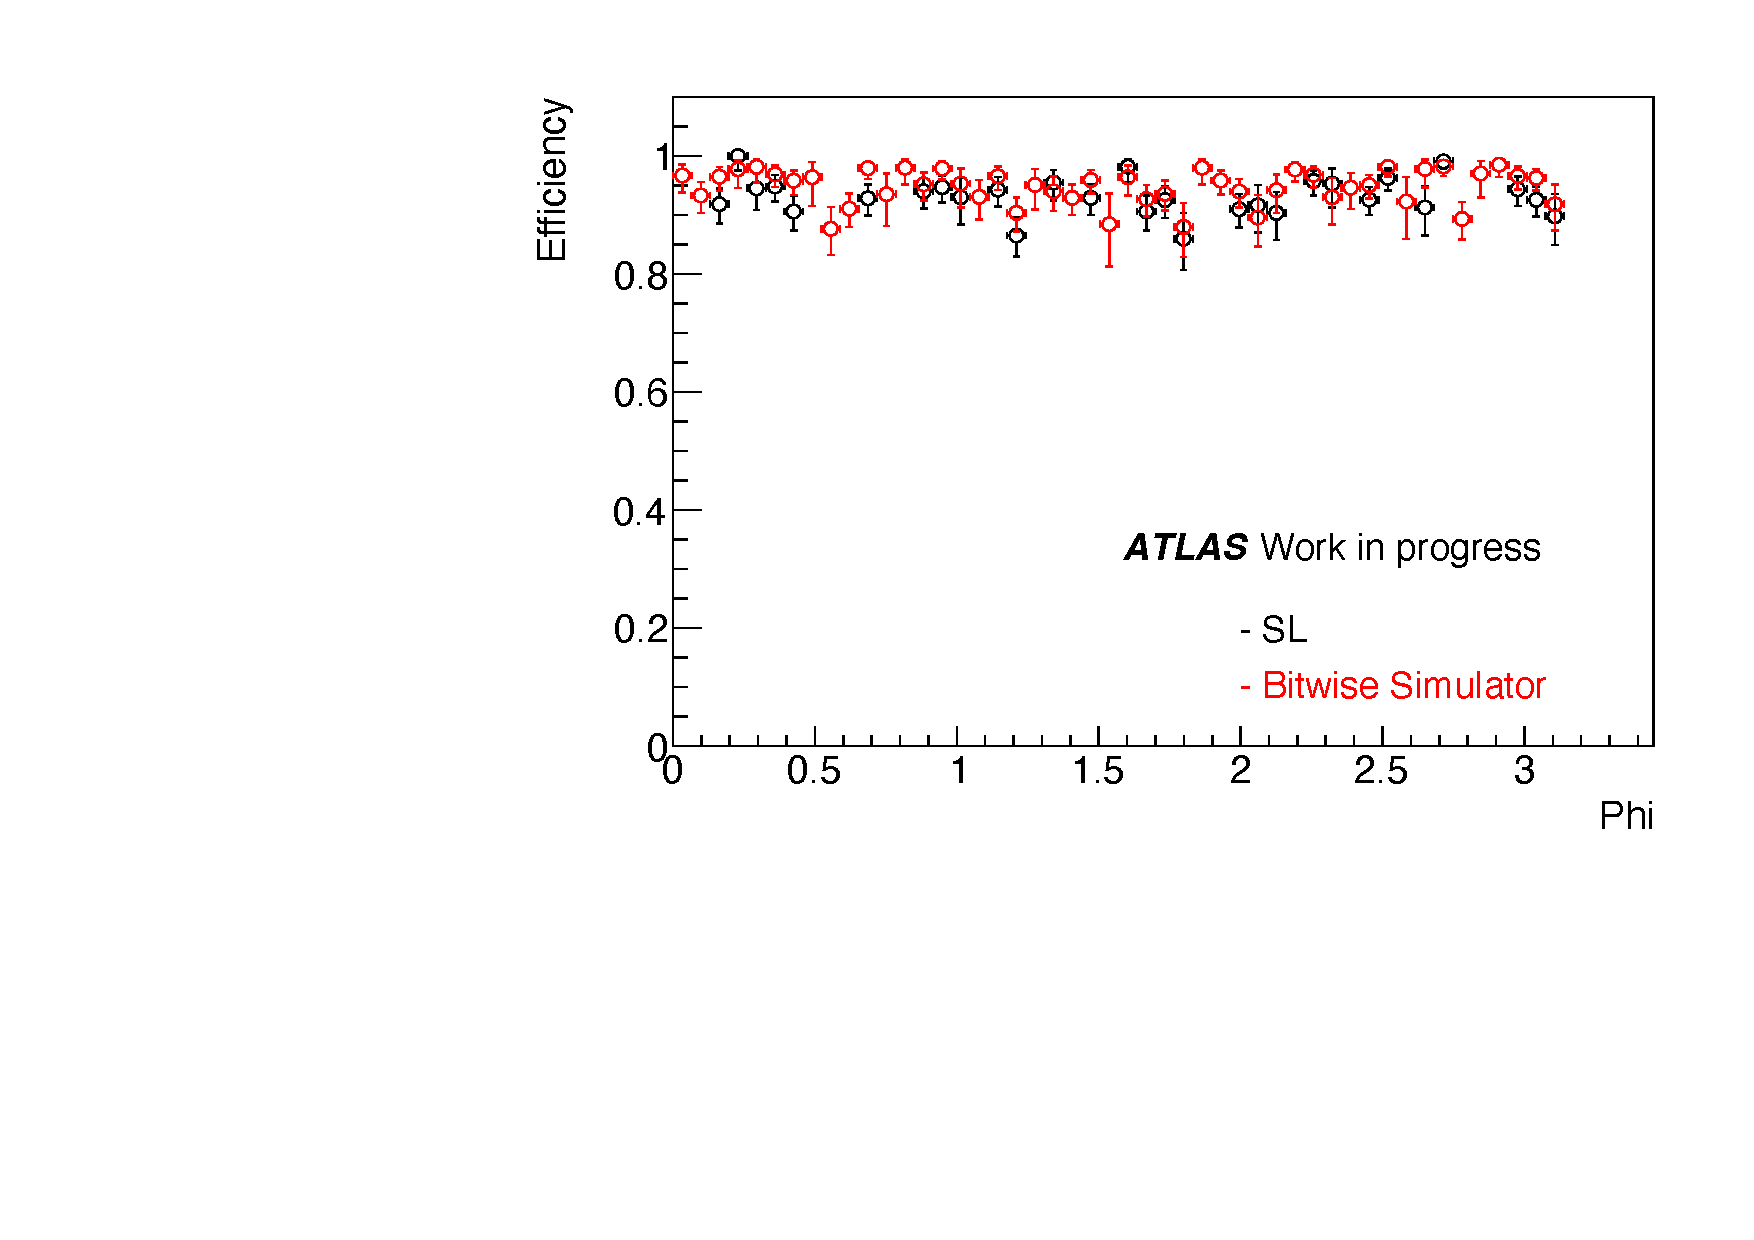
\includegraphics[height=10cm]{fig/Test/A_SM_ws_phi.pdf}
    \subcaption{Wire Strip Coincidence 検出効率の$\phi$依存性}
    \end{minipage}%
    \caption[Wire Strip Coincidenceの検出効率]{フォワード領域におけるWire Strip Coincidenceの検出効率。黒色のプロットが実機出力、赤色のプロットがBitwiseシミュレータの出力を表す。フォワード領域のトリガー検出効率は93.5 \%であり、先行研究と矛盾のない結果が得られた。トリガー効率の$\eta$依存性に着目すると、$\eta\sim1.95、2.2$付近で5 \%のInefficiencyが見られる。}
    \label{SM_A_WS}
\end{figure}

図\ref{SM_A_WS_turnon}にWire Strip Coincidenceの$p_\mathrm{T}$ごとの検出効率を示す。赤色、青色、緑色、ピンクの各カーブは、それぞれがトリガー閾値20 GeV、15 GeV、10 GeV、5 GeVと判断されたイベントの割合を示しており、一般にこのような図をターンオンカーブという。どの\pt 閾値に対してもプラトー領域のefficiencyは93.5 \%程度であり、先行研究\cite{mt_kawamoto}の結果と一致している (図\ref{Soft_WS})。実機の結果とBitwiseシミュレーターの結果も概ね一致している。

一方、先行研究の結果と比べて、Efficiencyの立ち上がりが緩やかで、\pt $\,$20 GeV以下のミューオンに対する除去効率が期待されるより低いことが明らかになった。\footnote{先行研究では、Bitwiseではなくフロートレベルでのソフトウェアシミュレーションを行なっている。また先行研究ではEfficiencyの分母としてOfflineで再構成されたミューオンのイベント数を採用しているのに対し、本件研究ではTruthのイベント数を採用している。}
例えば、Wire Segment Reconstructionで不当に$\Delta\theta$を小さく見積もってしまうと、このような振る舞いが生じ得る。今後、Segment Reconstructionの出力の絶対値も含めて、先行研究と比較するなどより詳細な調査をして、原因の解明を行う。

この結果を得るまでに、本研究によってWire Segment Reconstructionの問題点を発見し、修正を行なった。詳細をAppendix \ref{sec:appendix:MC-test}に記述する。また、プラトー領域に存在する6.5 \%程度のInefficiencyの原因についても調査を行った。この調査結果についてはAppendix \ref{sec:appendix:plateau}に詳細を記述する。
% さらに、今回の試験ではTGC検出器は理想位置と呼ばれる設計段階の位置に設置されていることを仮定して、モンテカルロデータやLUTを作成した。実験本番ではTGC検出器はアライメントの誤差により理想位置からずれた場所に設置される。このずれがトリガー効率にどれほど影響を与えるか調査した。その結果をAppendix{sec:appendix:alignment  \(\)}に示す。

\begin{figure}
    \begin{minipage}[b]{\linewidth}
    \centering
    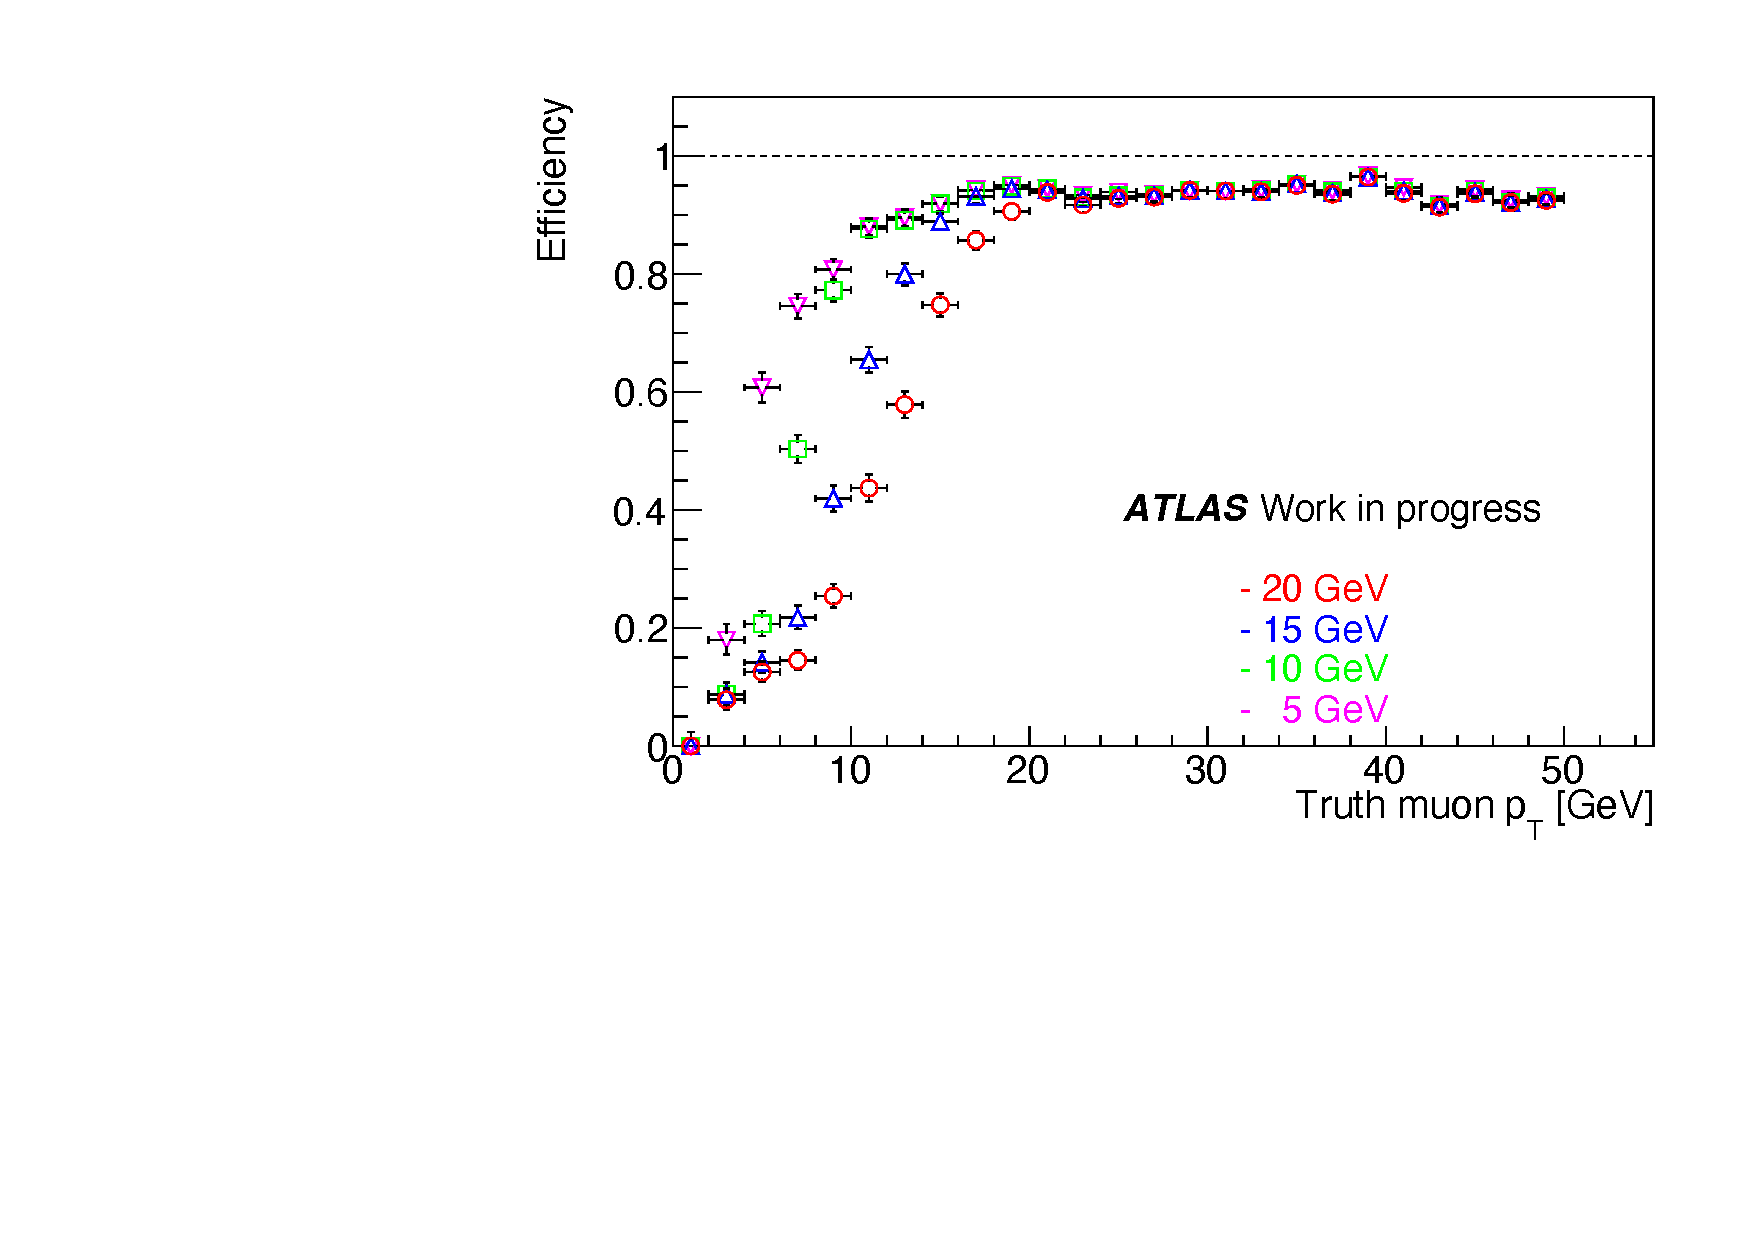
\includegraphics[height=10cm]{fig/Test/A_SM_ws_turn.pdf}
    \subcaption{実機の結果}
    \end{minipage}\\
    \begin{minipage}[b]{\linewidth}
    \centering
    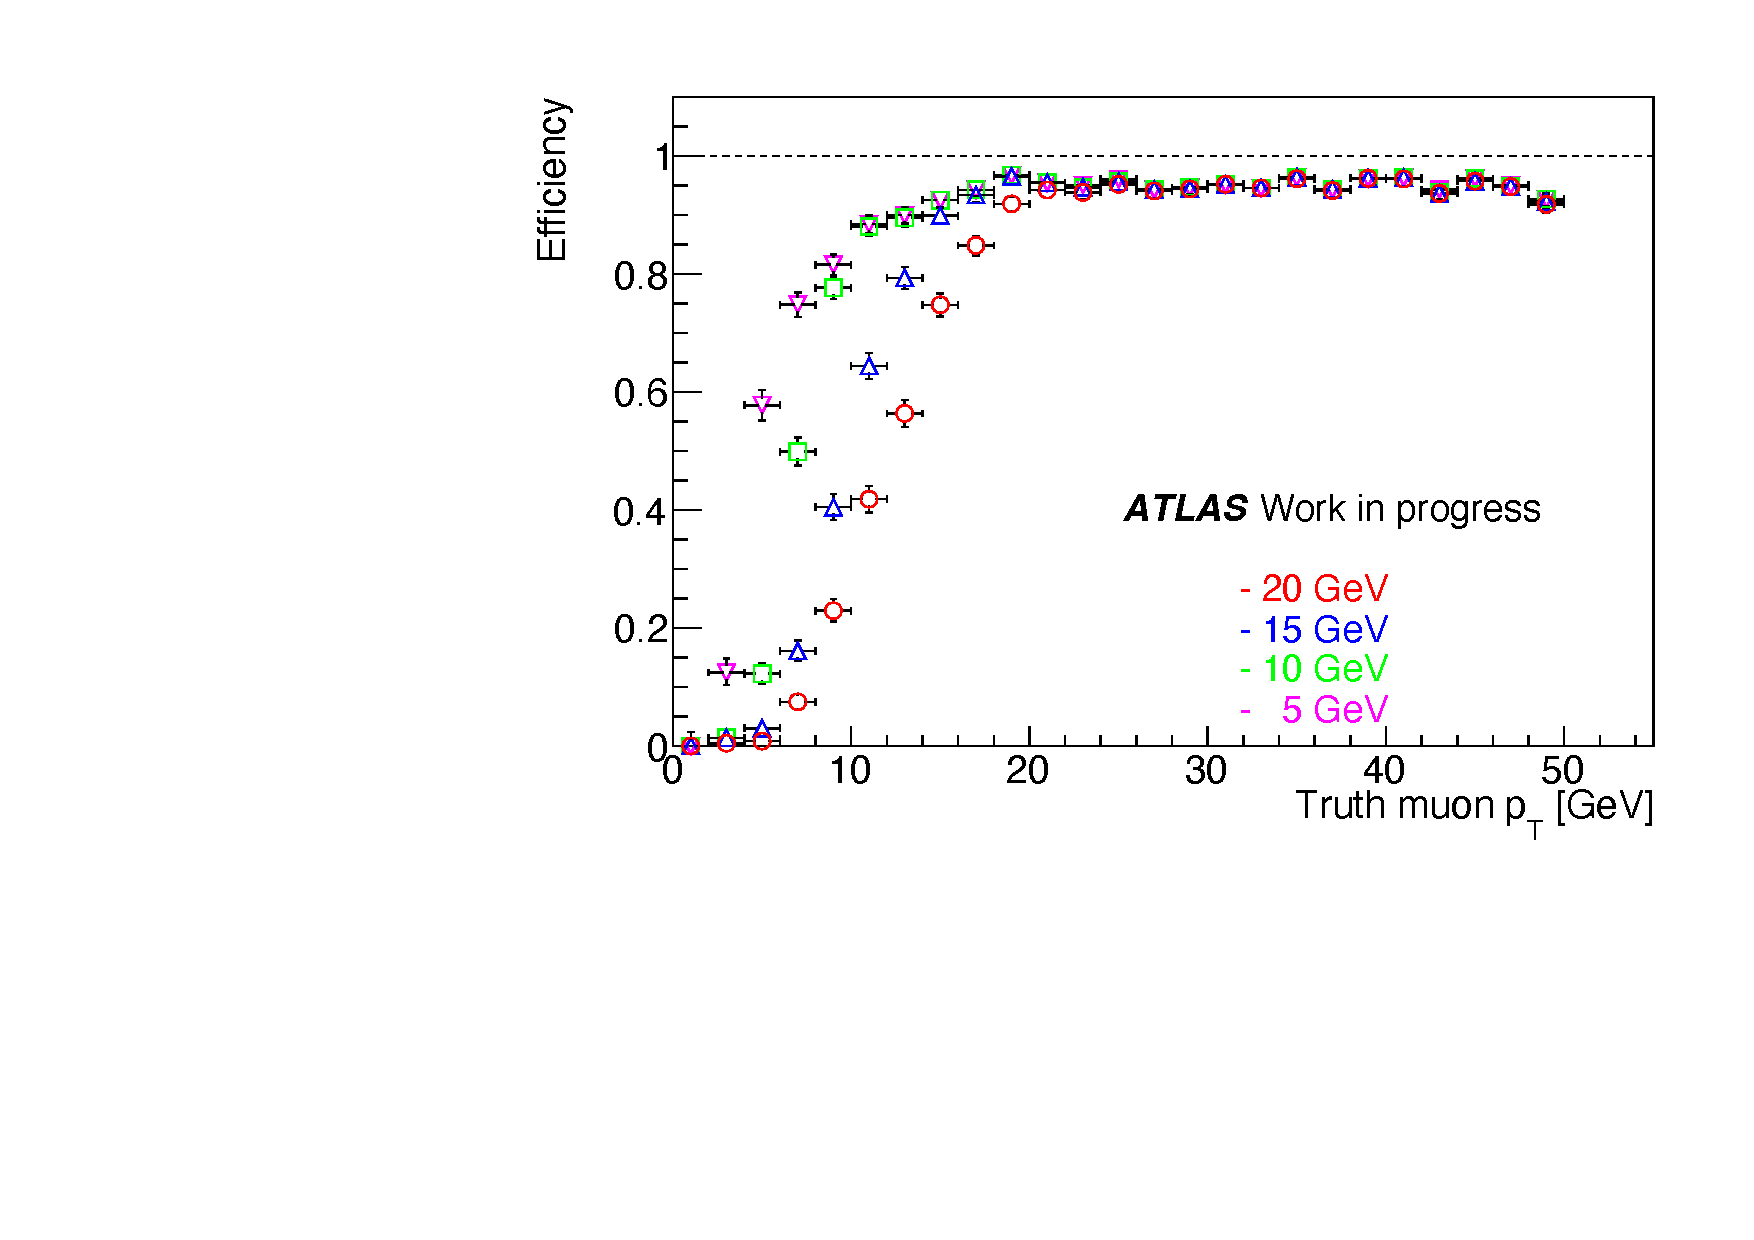
\includegraphics[height=10cm]{fig/Test/A_SM_ws_turnon_bitwise.pdf}
    \subcaption{Bitwiseシミュレーターの結果}
    \end{minipage}%
    \caption[Wire Strip Coincidenceの$p_\mathrm{T}$ごとの検出効率]{Wire Strip Coincidence フォワード領域における$p_\mathrm{T}$ごとの検出効率。赤色、青色、緑色、ピンクの各プロットは、それぞれが $p_{\mathrm{T}}$ 閾値20 GeV、15 GeV、10 GeV、5 GeVと判断されたイベントの割合を示している。プラトー領域のefficiencyはいずれの$p_{\mathrm{T}}$閾値に対しても93.5 \%程度であり、先行研究の結果と一致している。}
    \label{SM_A_WS_turnon}
\end{figure}

\subsection*{まとめ}
本研究では、任意のデータセットに対するトリガー応答を高速で計算するシングルボード試験システムを開発し、無限運動量飛跡やモンテカルロデータを用いてトリガーロジックの性能評価試験を行った。その結果、Wire Strip Coincidenceまでの大部分の領域が期待される性能を有していることを初めて確認することができた。また、シングルボード試験システムとBitwiseシミュレーションの比較により、問題を系統的に特定する検証基盤も構築したことで、これまで発見が困難だった論理回路やLUTの局所的な不具合を発見し、多くの問題点を解決することができた(Appendix \ref{sec:appendix:infinite-momentum-tracks}$\sim$ \ref{sec:appendix:MC-test}参照)。これからも、\ref{sec_IMT}節と\ref{sec_SingleMuon}で議論した残された課題に対して詳細な調査とデバッグを進めていくことで、ミューオントリガー実装の精度を高めていく。



